\subsection{External Interface Requirements}

\subsubsection{User Interfaces}
% In this section we present user interfaces for Students and Educators. 
% \begin{center}
%     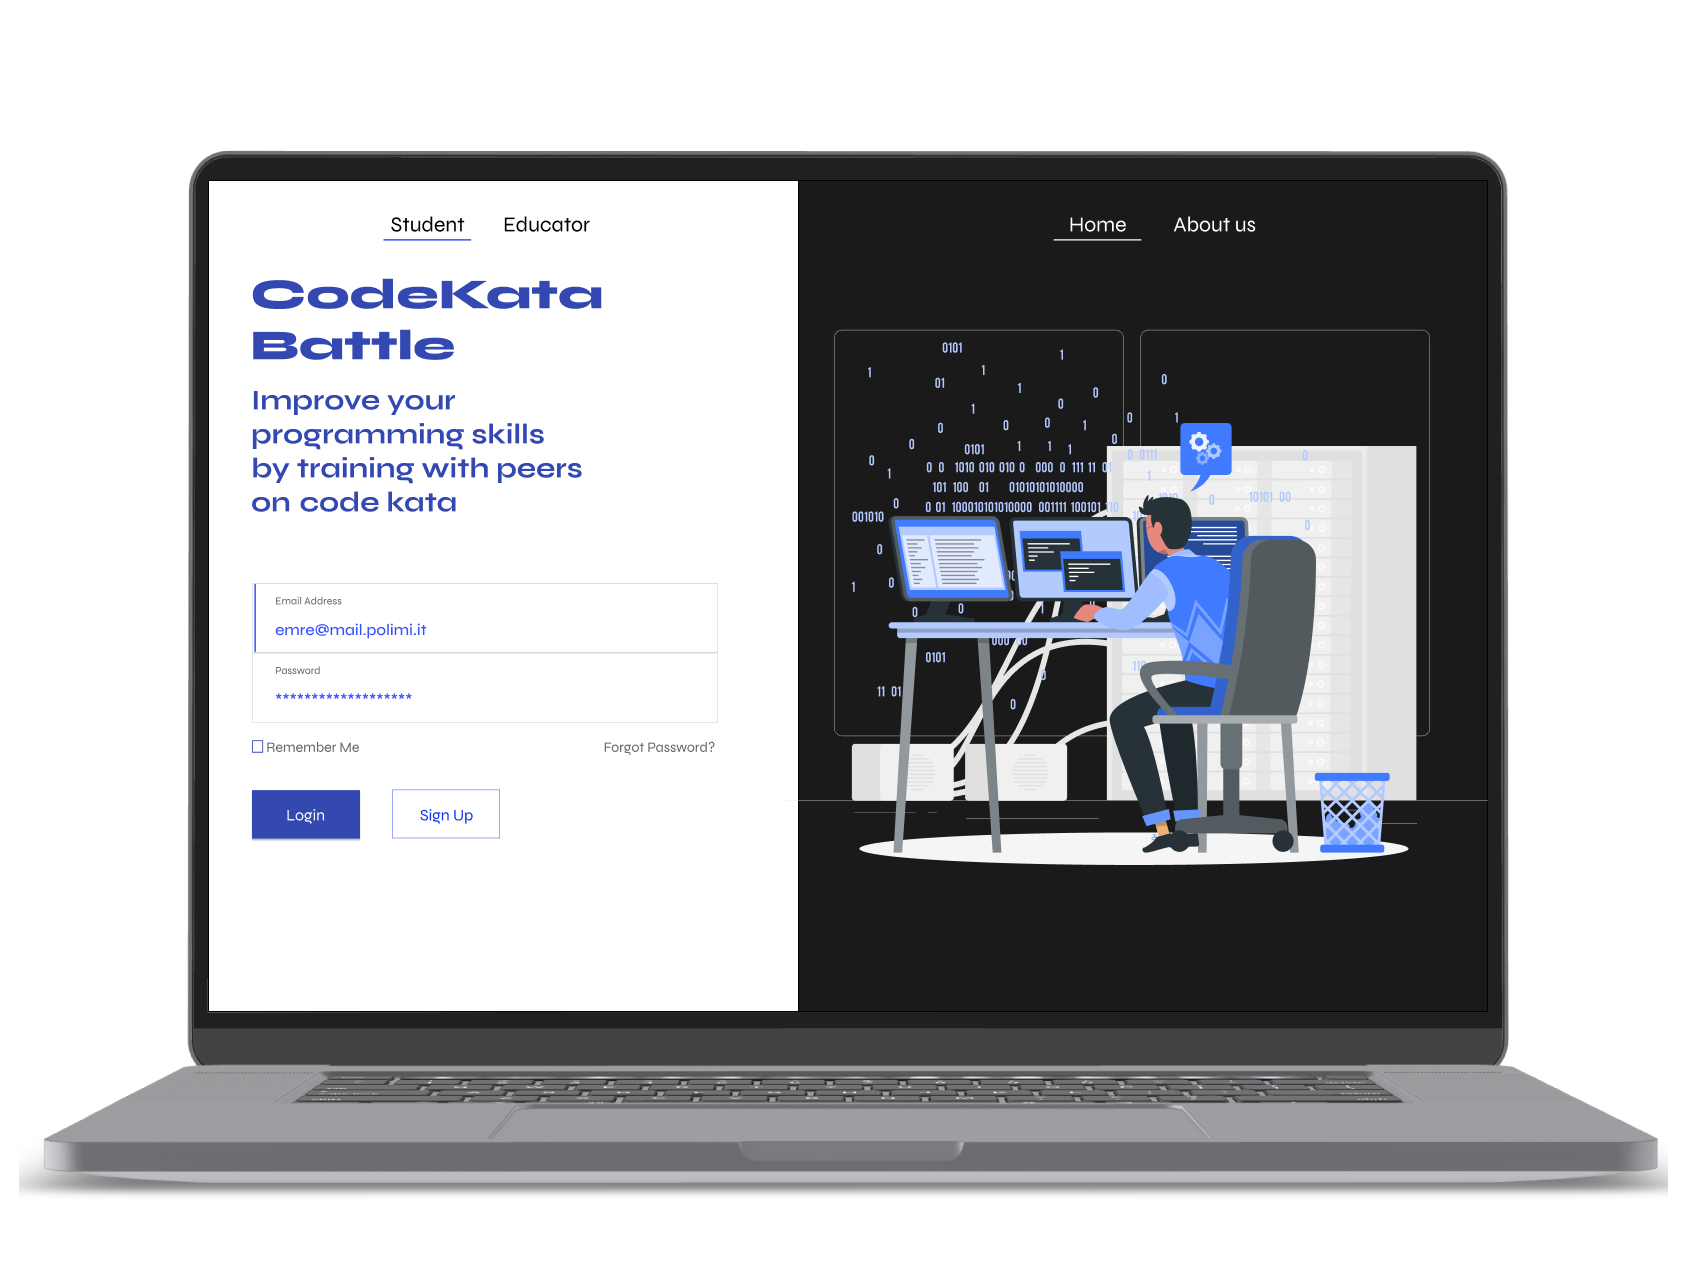
\includegraphics[scale=0.13]{Images/ui-ux/login-signup/student_login.png}
%     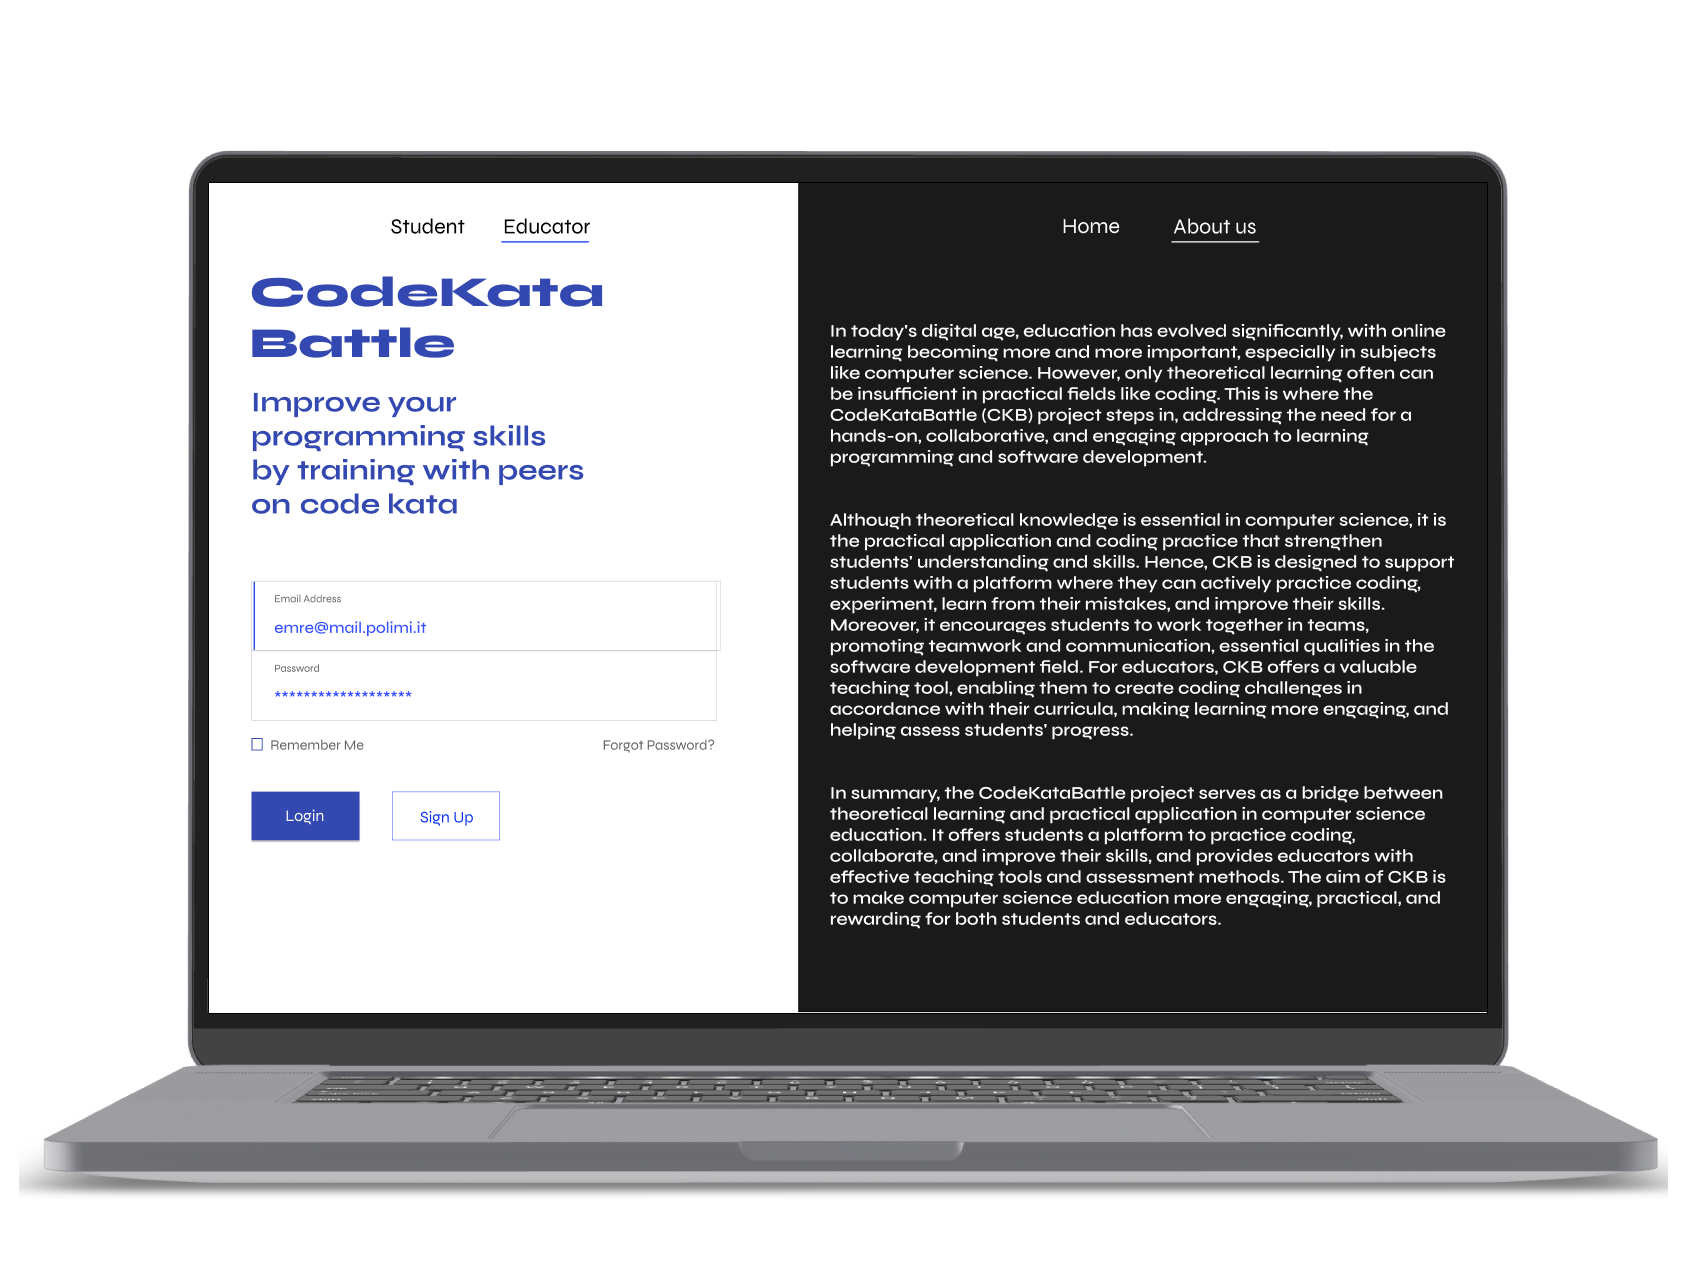
\includegraphics[scale=0.13]{Images/ui-ux/login-signup/educator_login.png}
% \end{center}
%     \begin{center}
%         (a) Login Screens
%     \end{center}
% \begin{center}
%     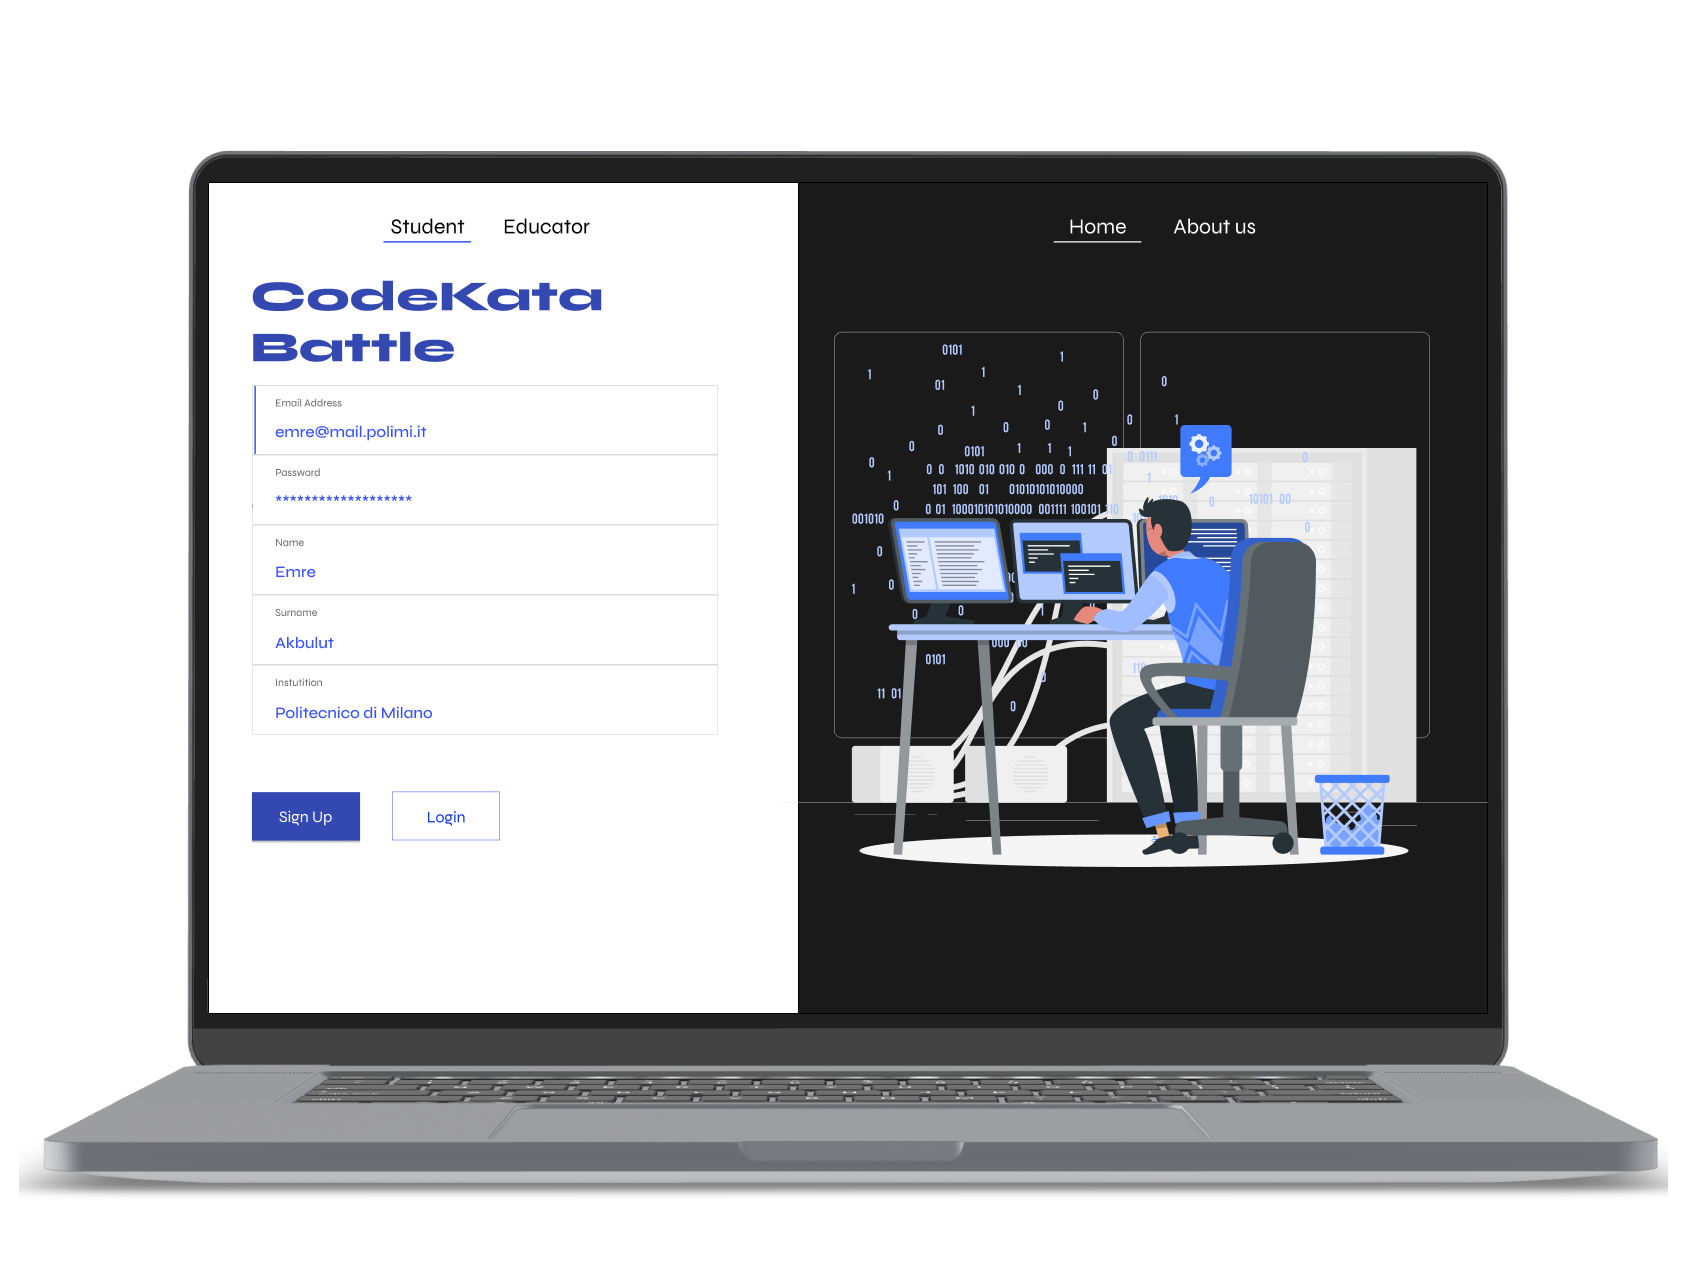
\includegraphics[scale=0.13]{Images/ui-ux/login-signup/student_signup.png}
%     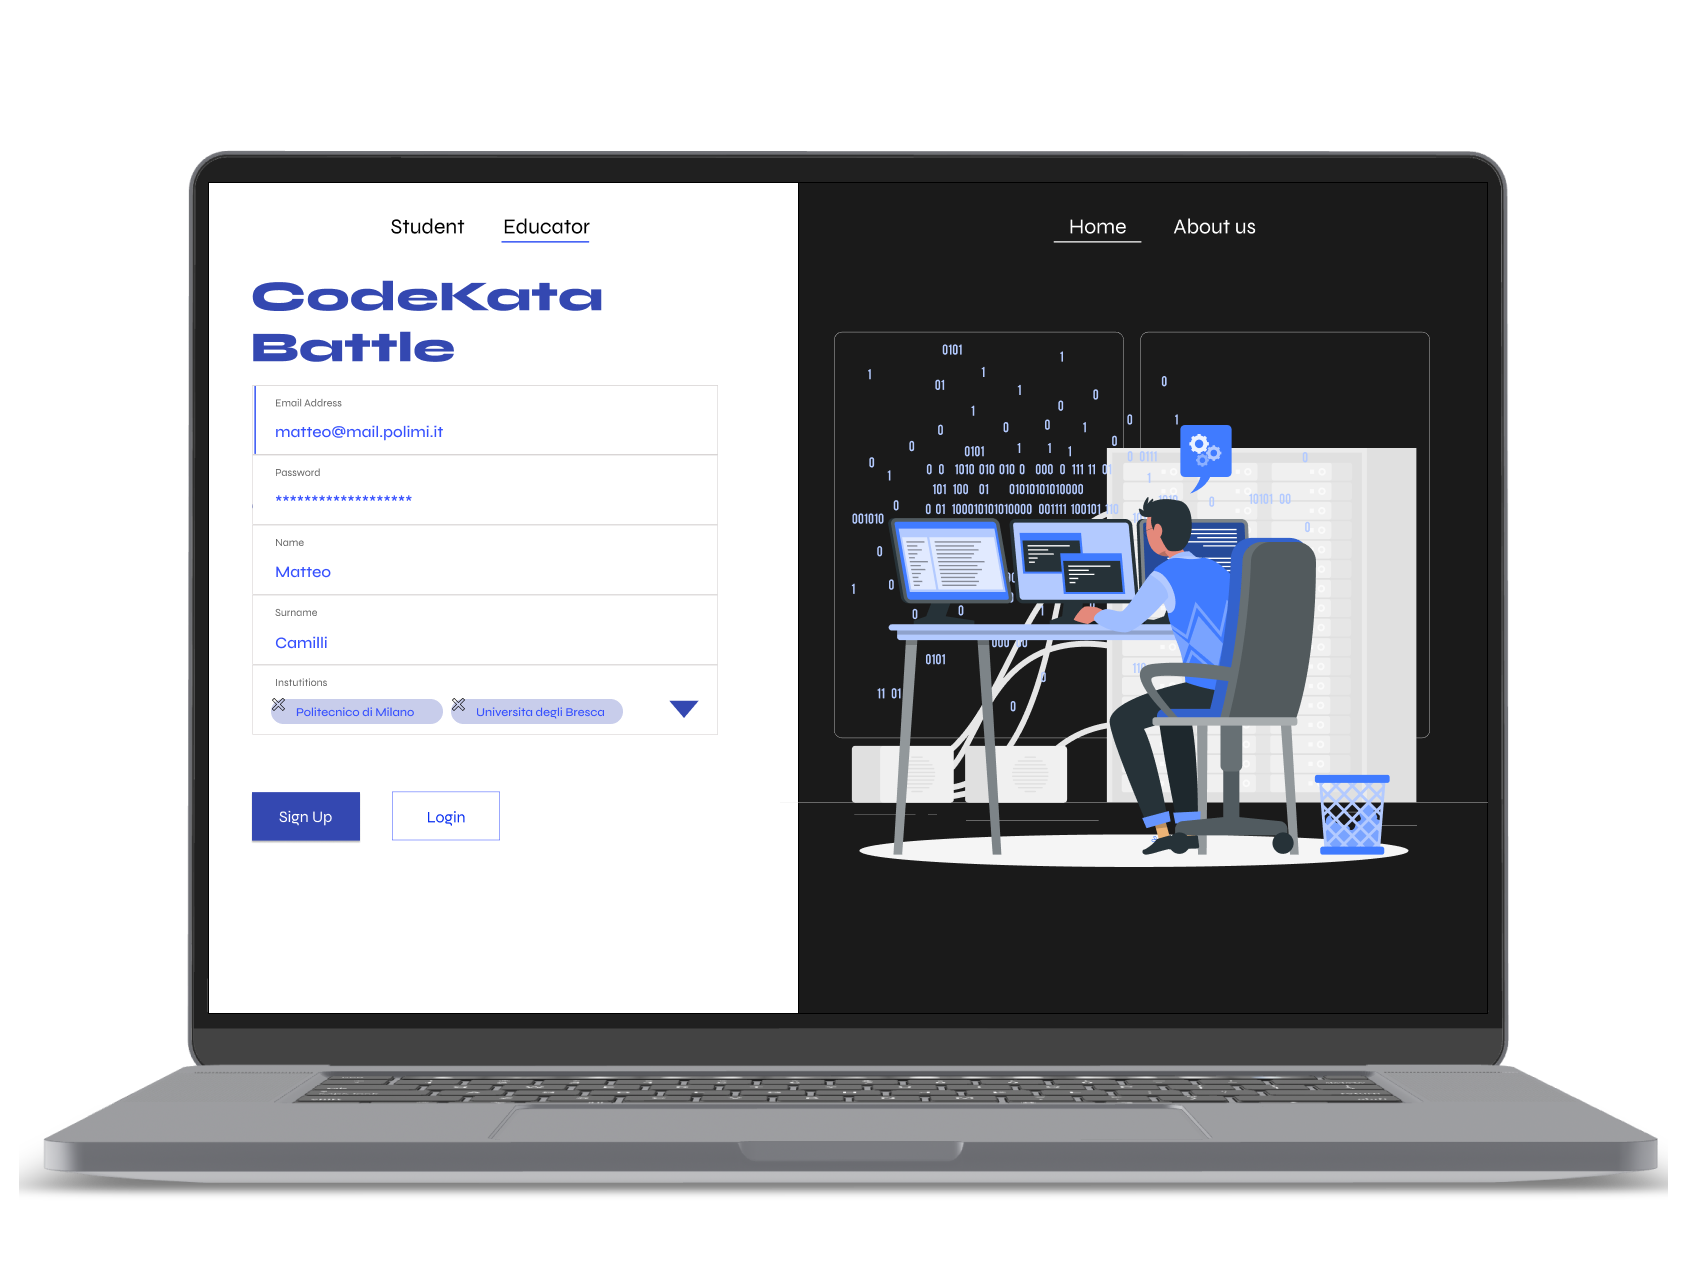
\includegraphics[scale=0.13]{Images/ui-ux/login-signup/educator_signup.png}
%     (a) Sign up Screens
% \end{center}
% \newpage
% \begin{center}
%     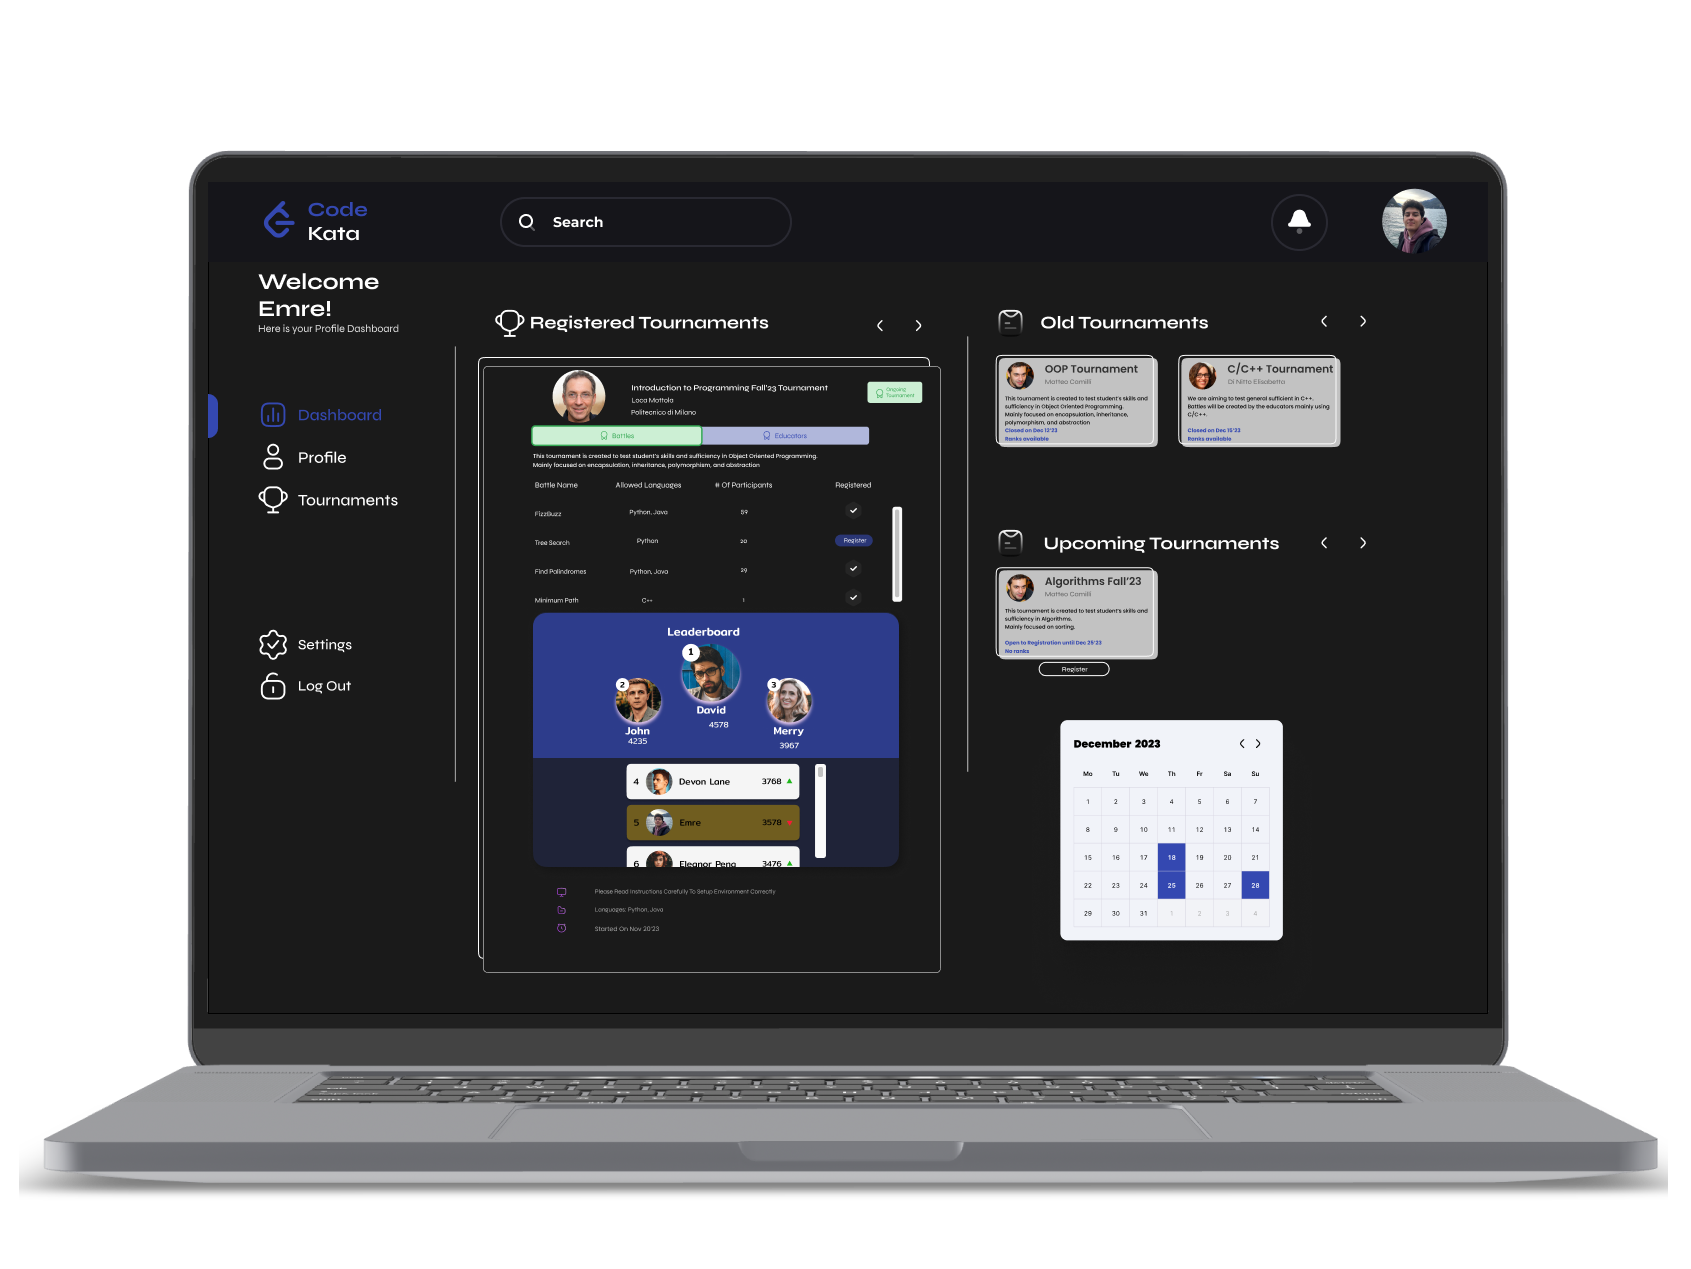
\includegraphics[scale=0.13]{Images/ui-ux/student_dashboard/student_dashboard_1.png}
%     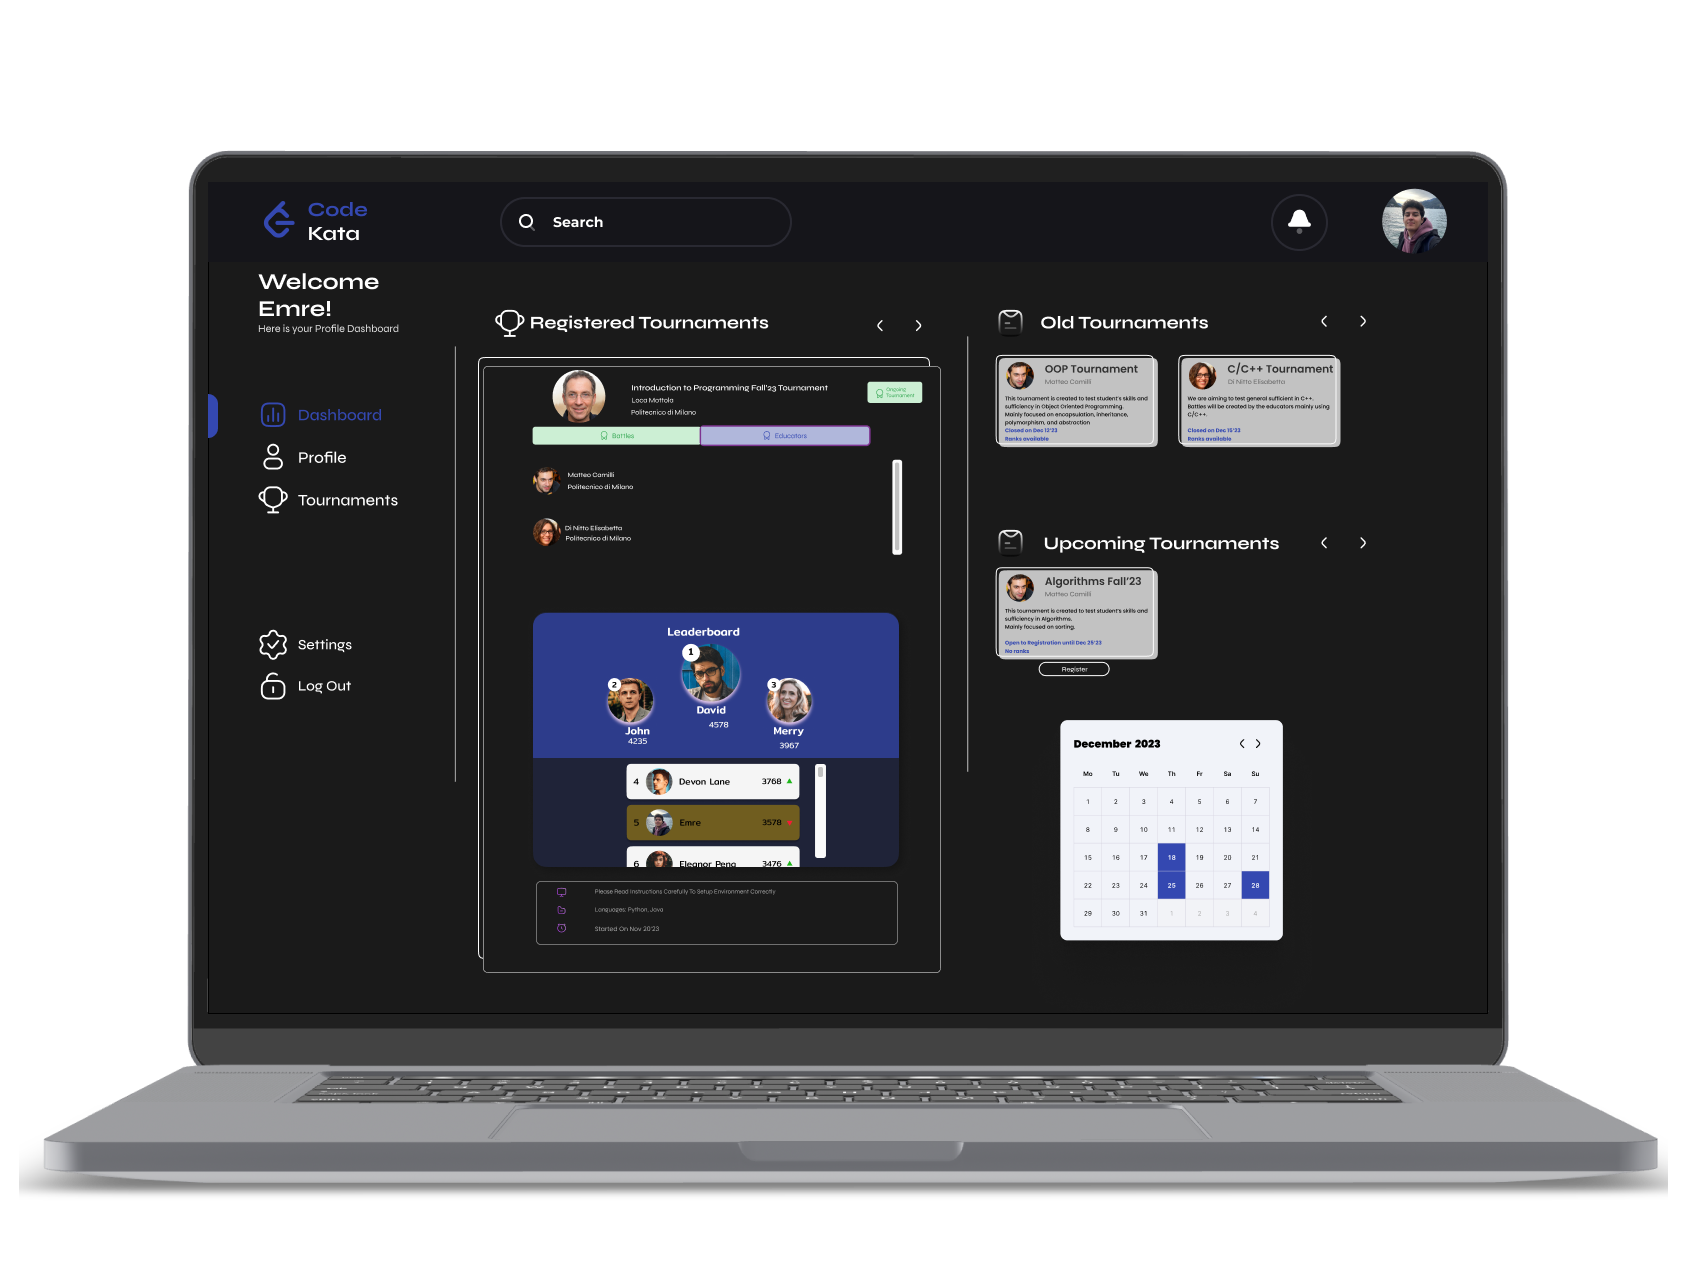
\includegraphics[scale=0.13]{Images/ui-ux/student_dashboard/student_dashboard_2.png}
%             (a) Student Dashboard
% \end{center}
% \begin{center}
%     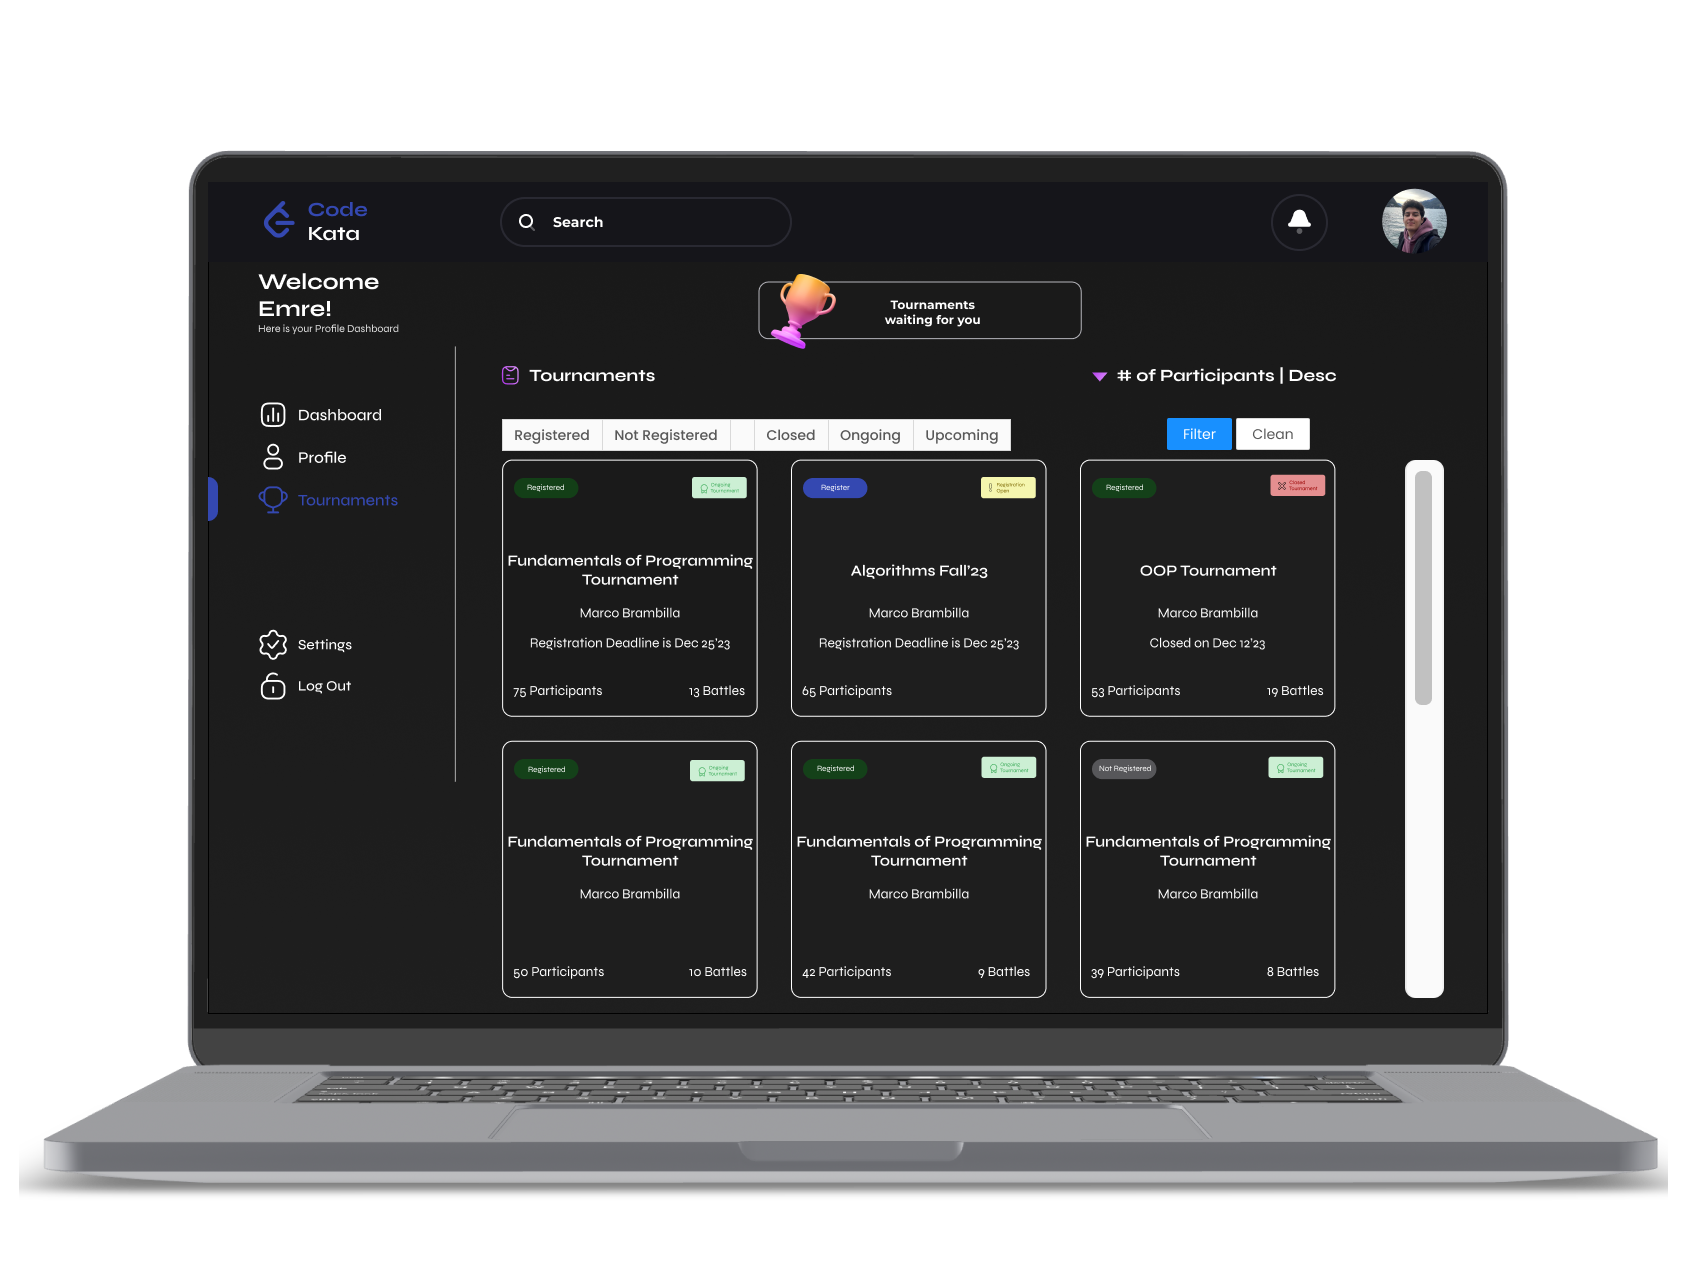
\includegraphics[scale=0.13]{Images/ui-ux/student_tournaments/student_tournaments_1.png}
%     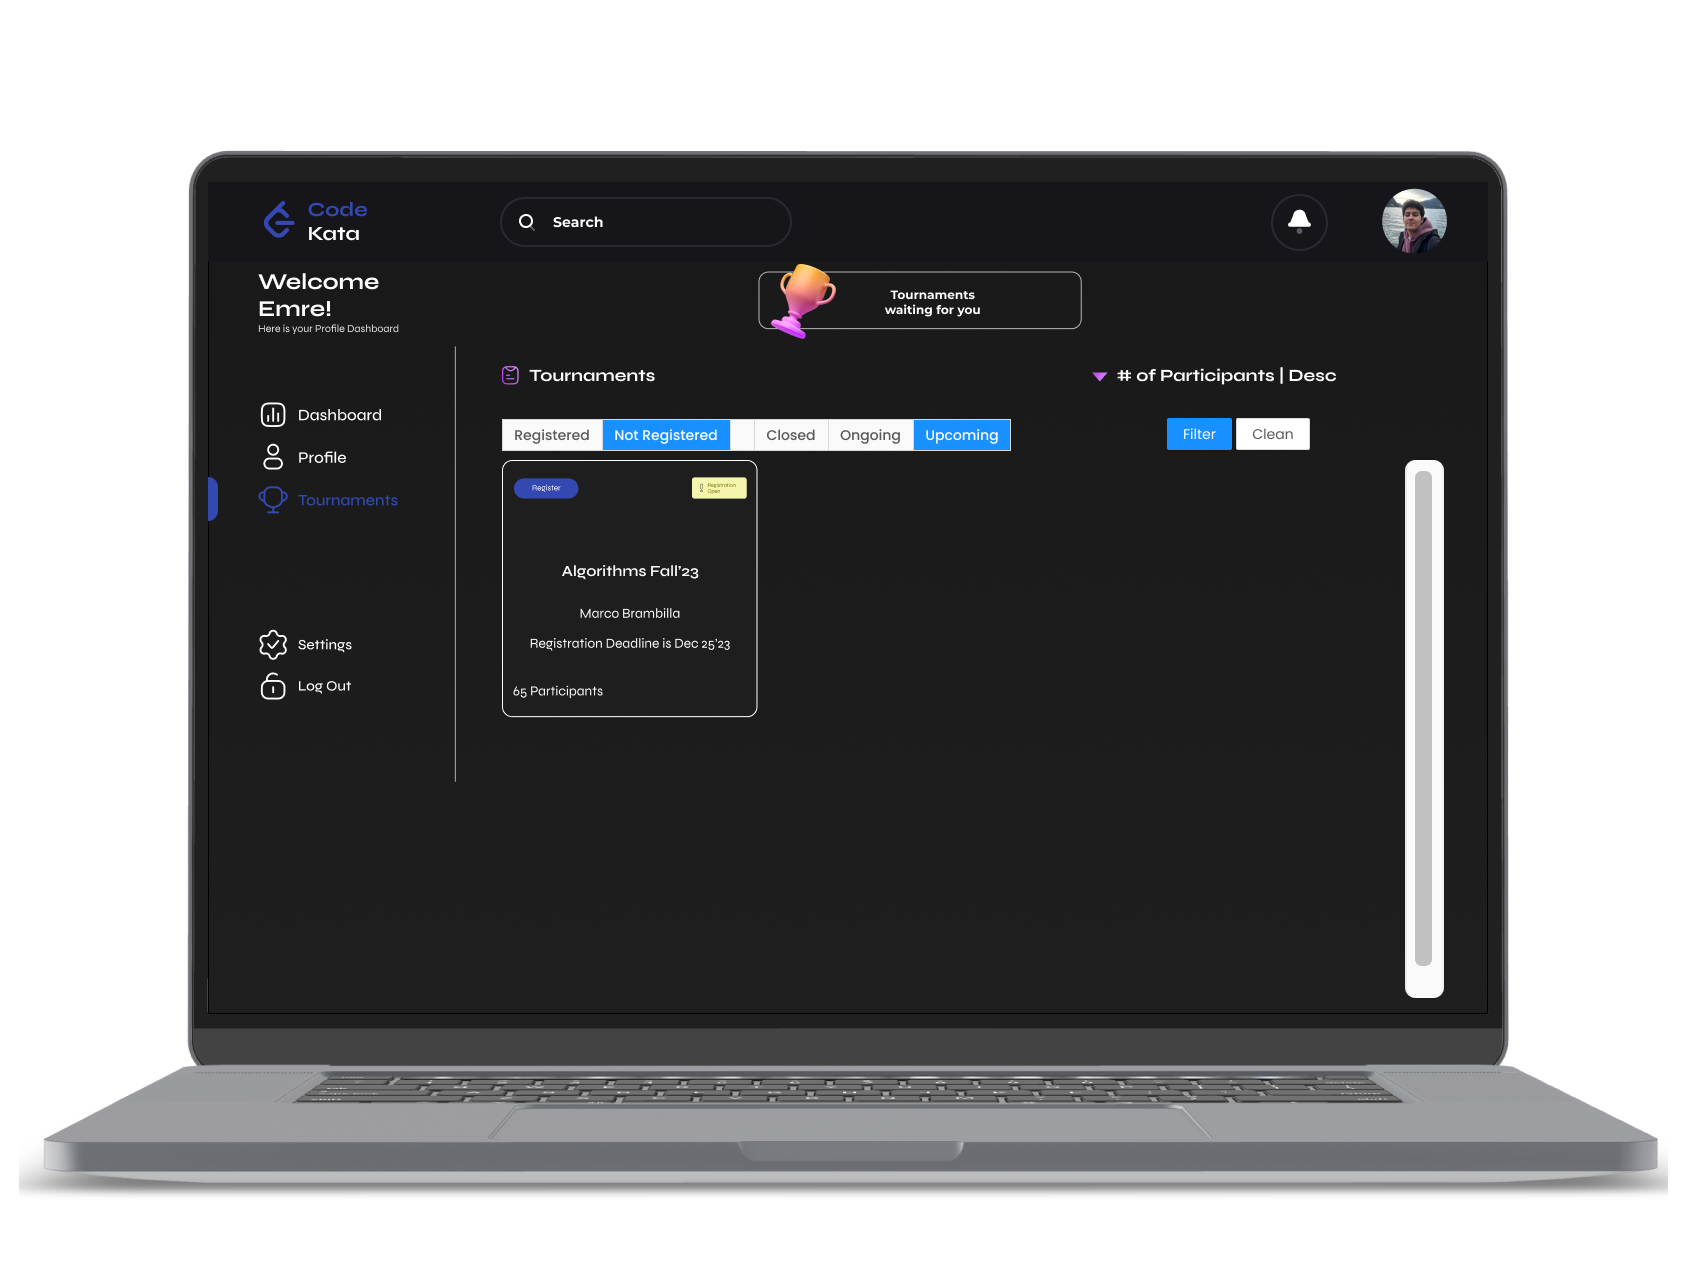
\includegraphics[scale=0.13]{Images/ui-ux/student_tournaments/student_tournaments_2.png}    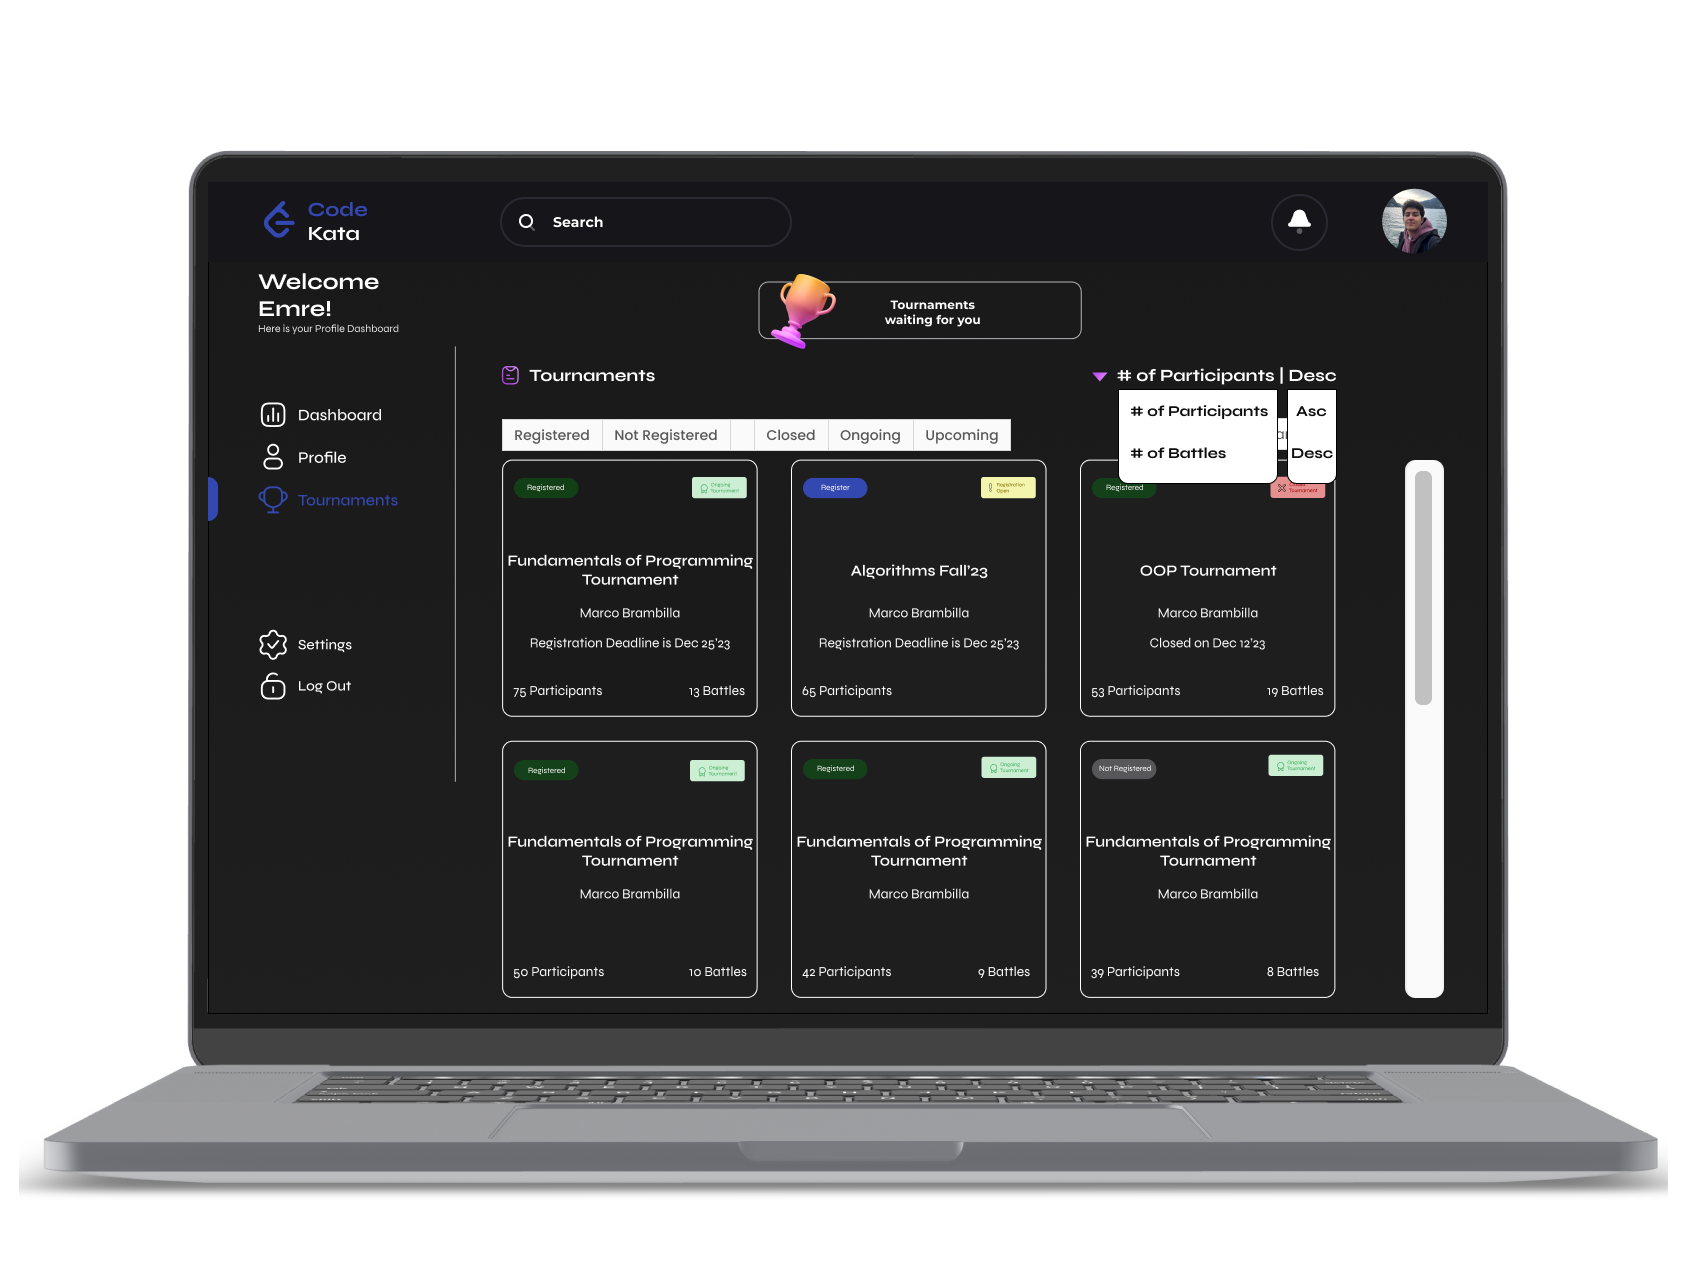
\includegraphics[scale=0.13]{Images/ui-ux/student_tournaments/student_tournaments_3.png}    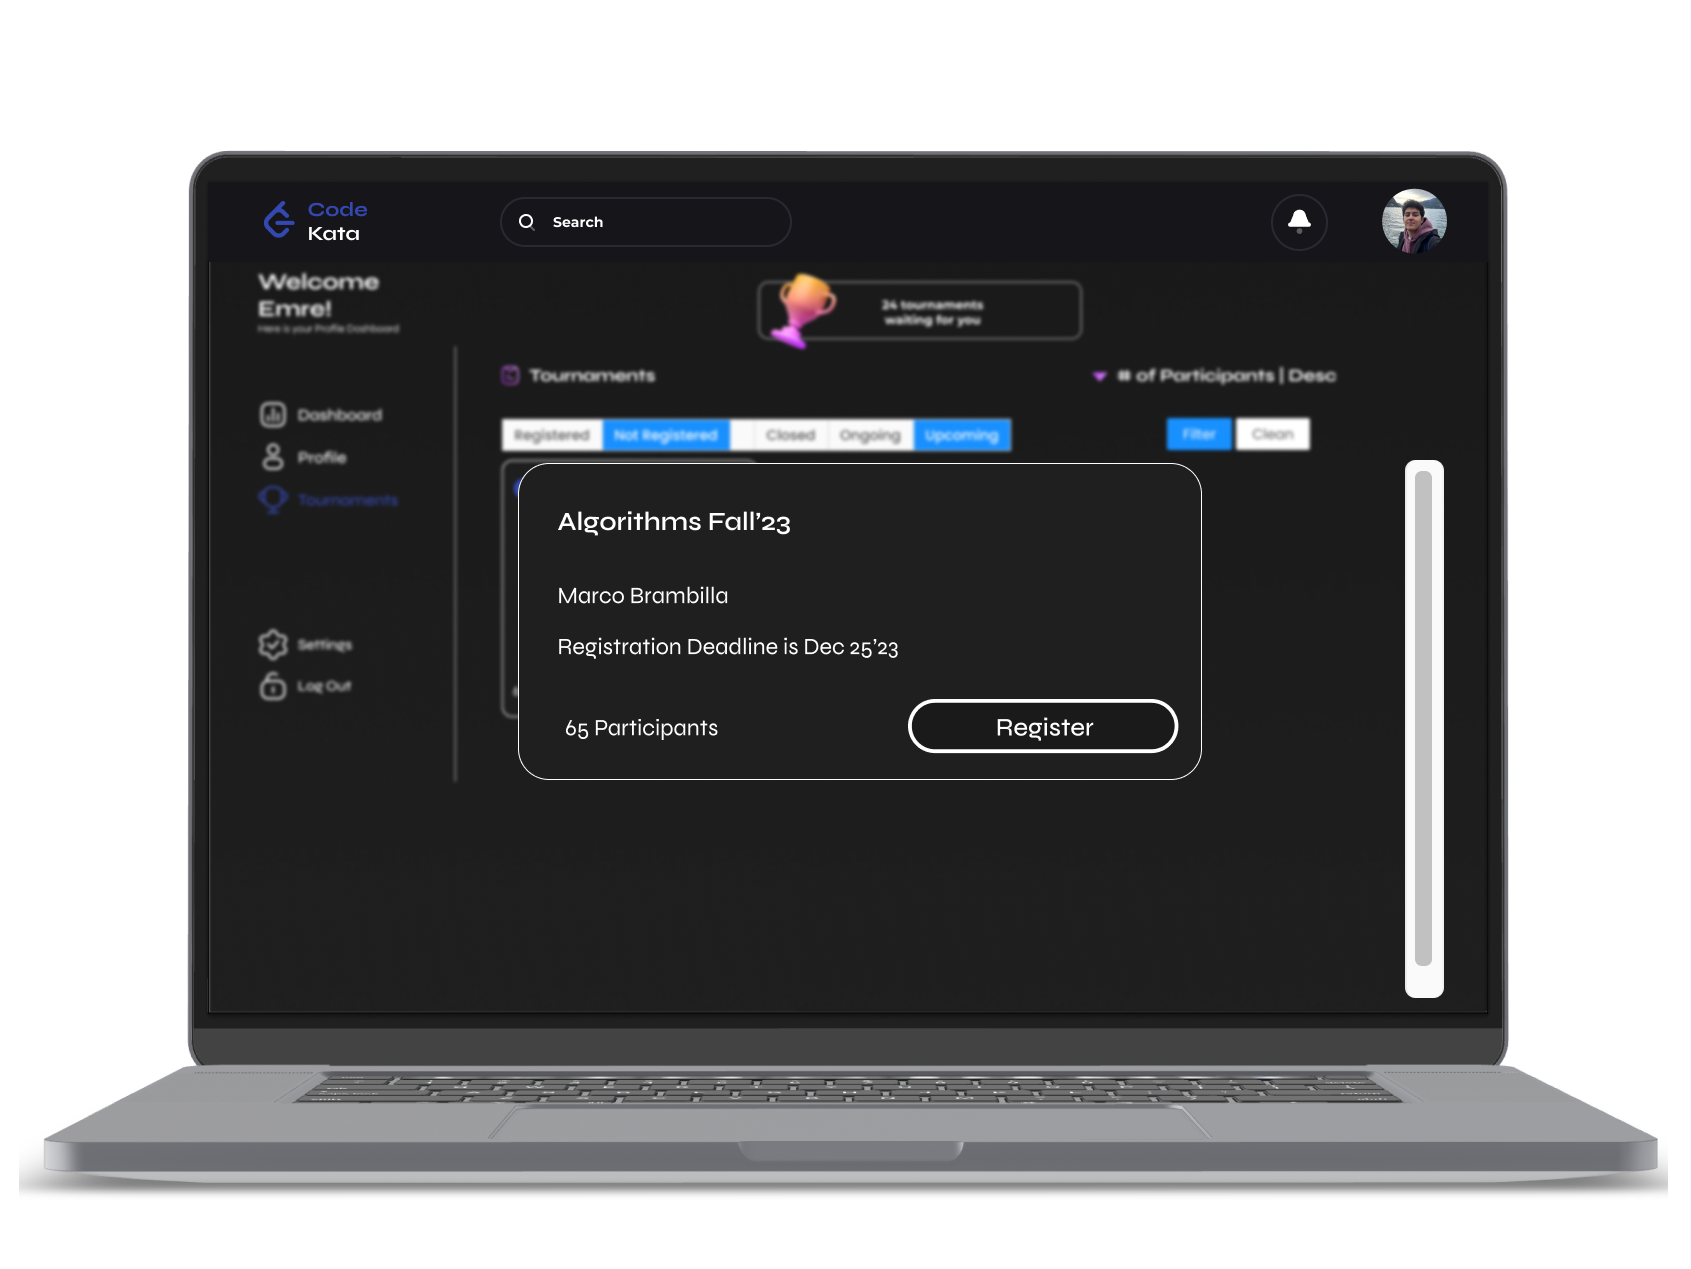
\includegraphics[scale=0.13]{Images/ui-ux/student_tournaments/student_tournaments_4.png}
%         (a) Student Tournaments
% \end{center}

% \begin{center}
%     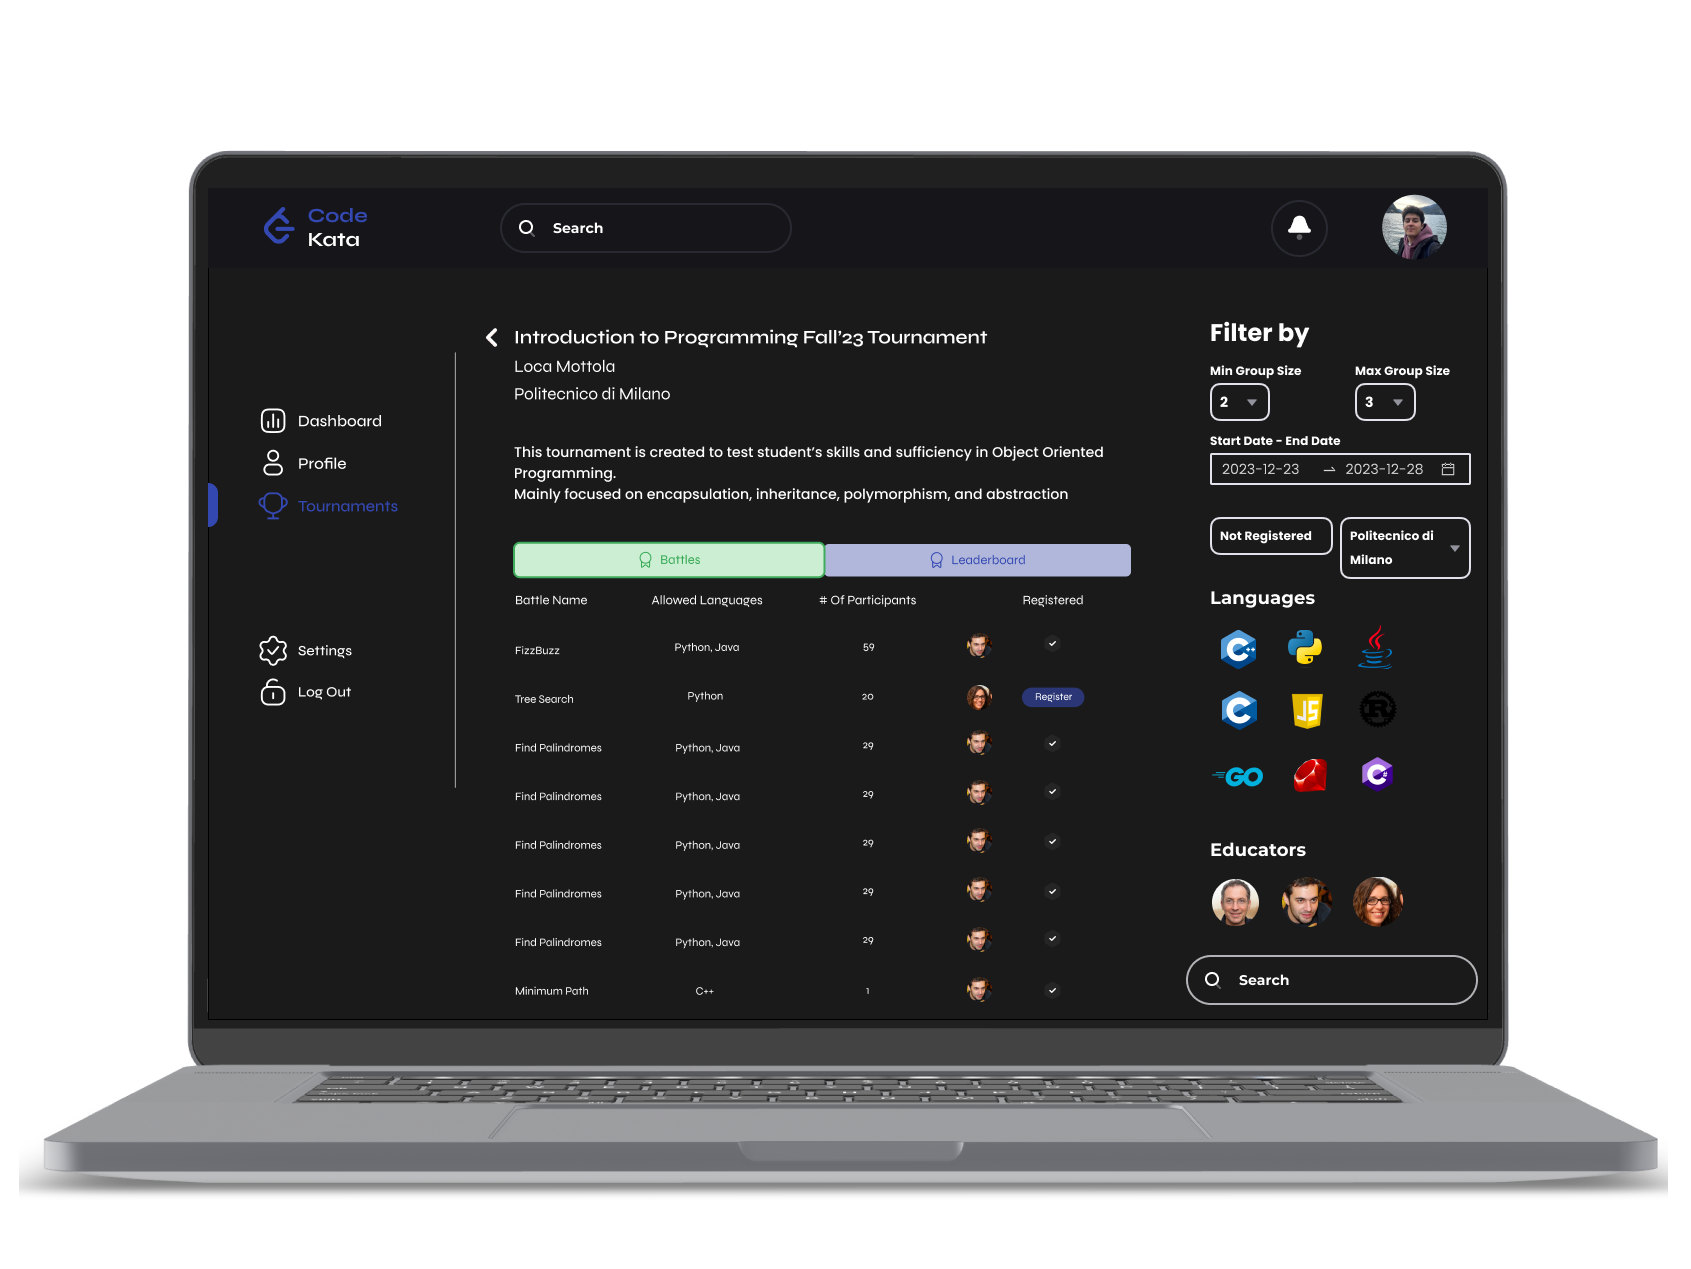
\includegraphics[scale=0.13]{Images/ui-ux/student_tournament/student_tournament_1.png}
%     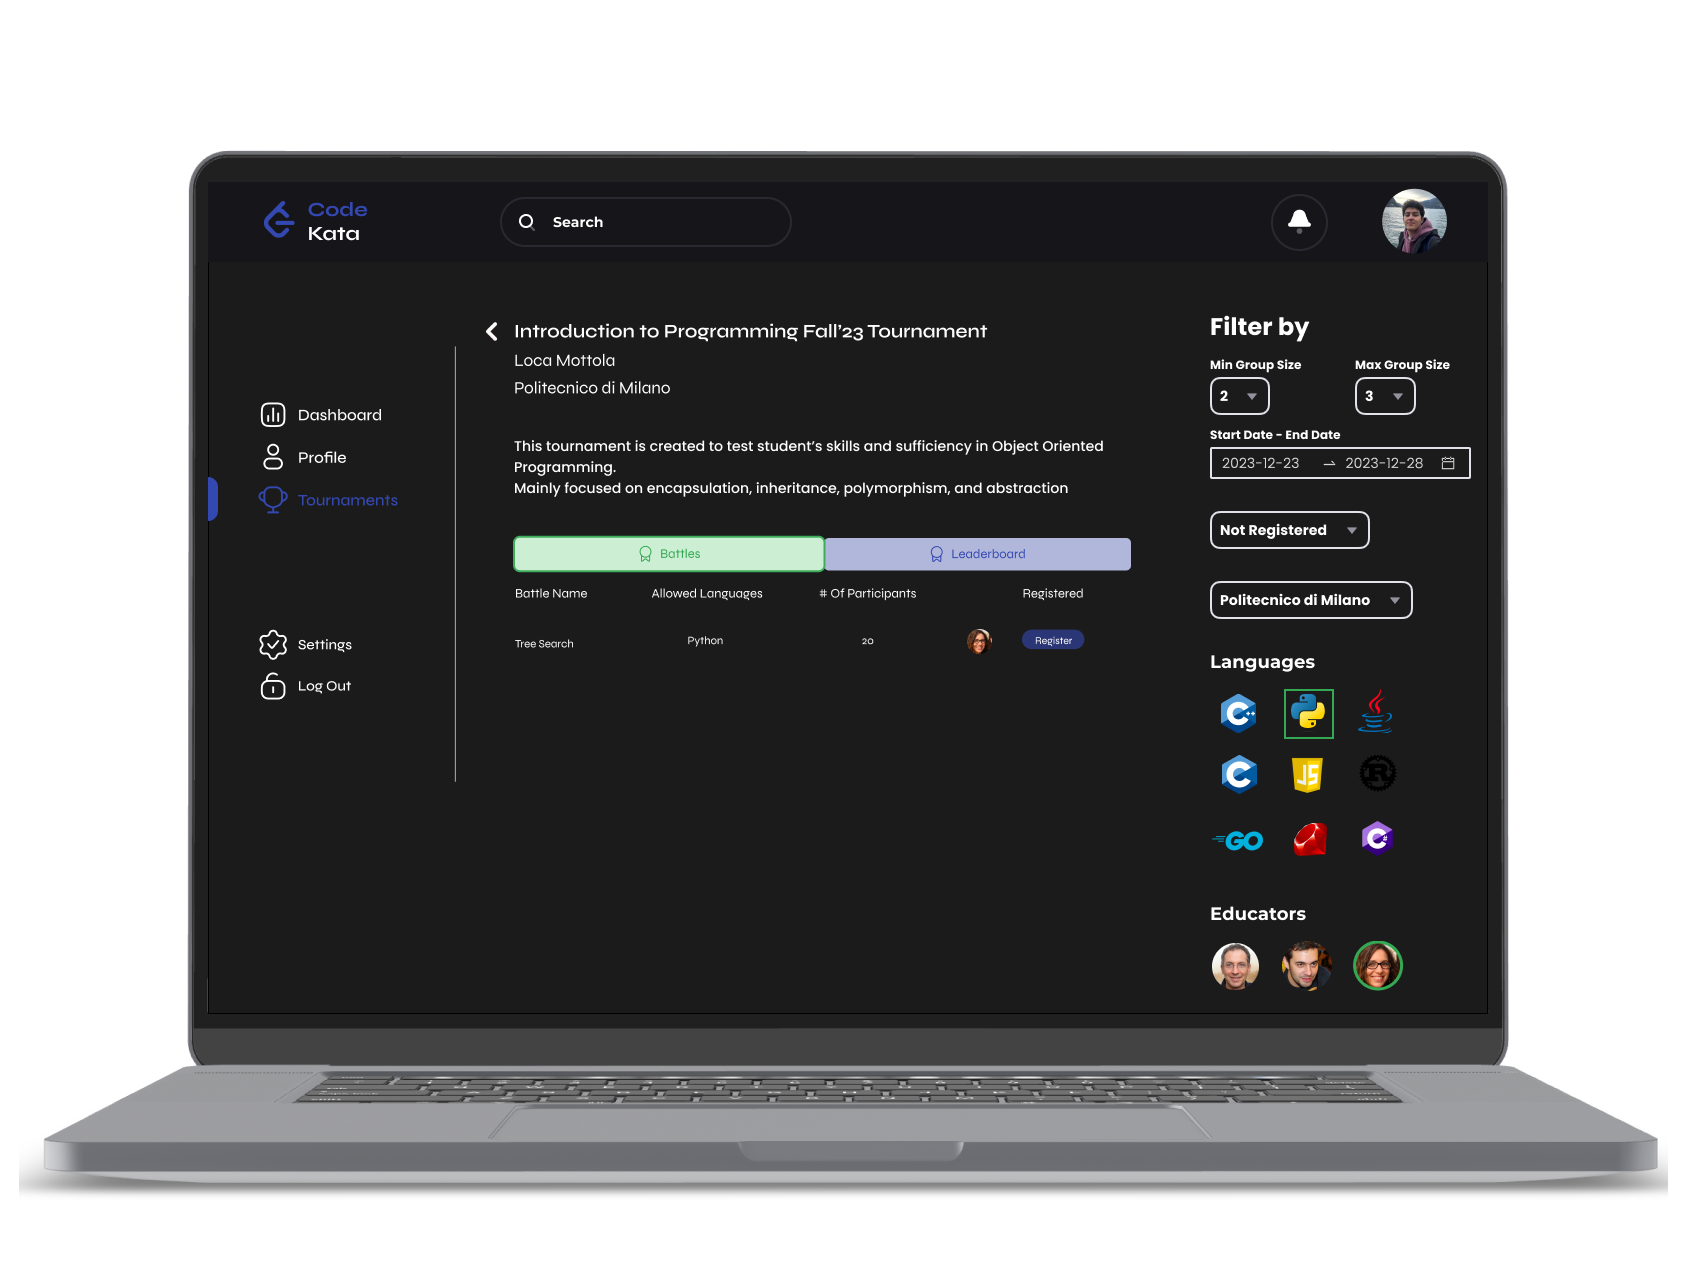
\includegraphics[scale=0.13]{Images/ui-ux/student_tournament/student_tournament_2.png}    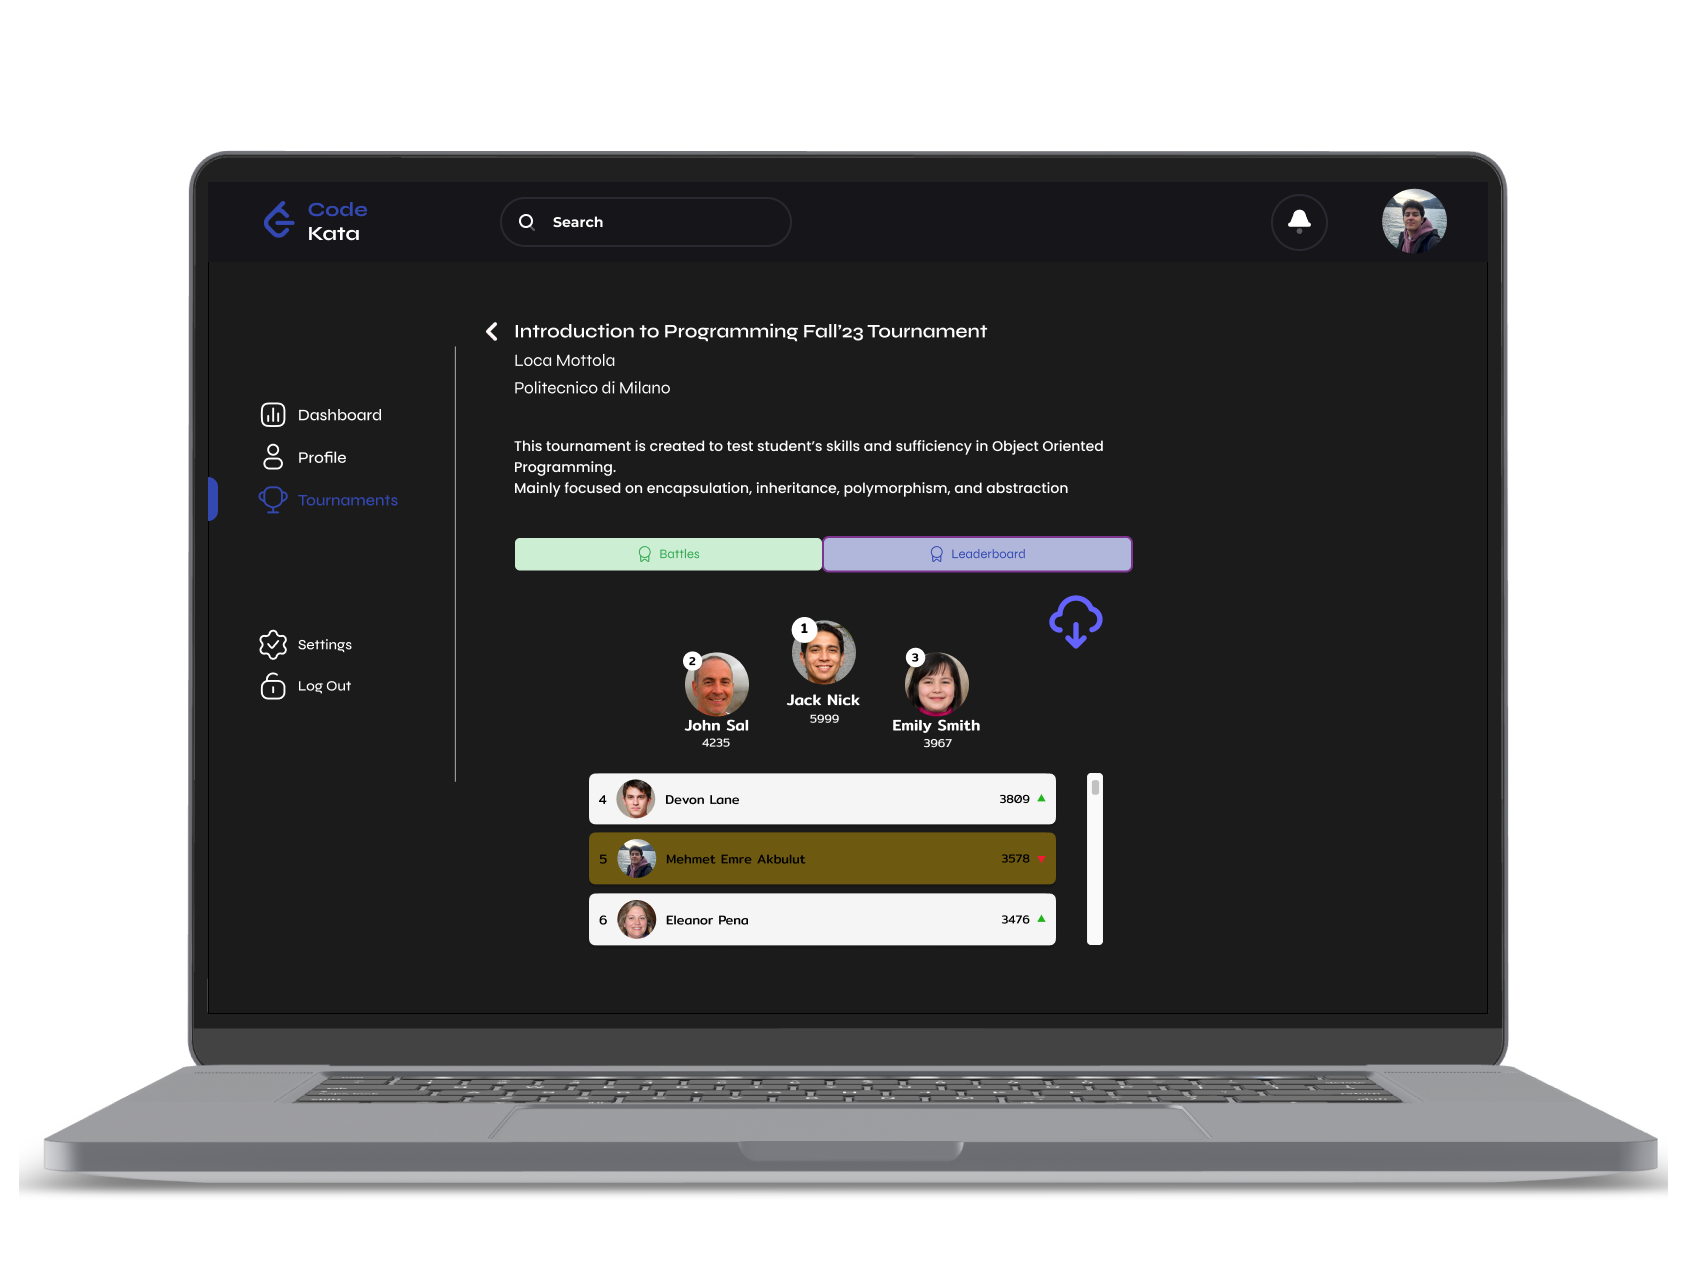
\includegraphics[scale=0.13]{Images/ui-ux/student_tournament/student_tournament_3.png} 
%     \\ (a) Student and A Tournament
% \end{center}
% \newpage
% \begin{center}
% 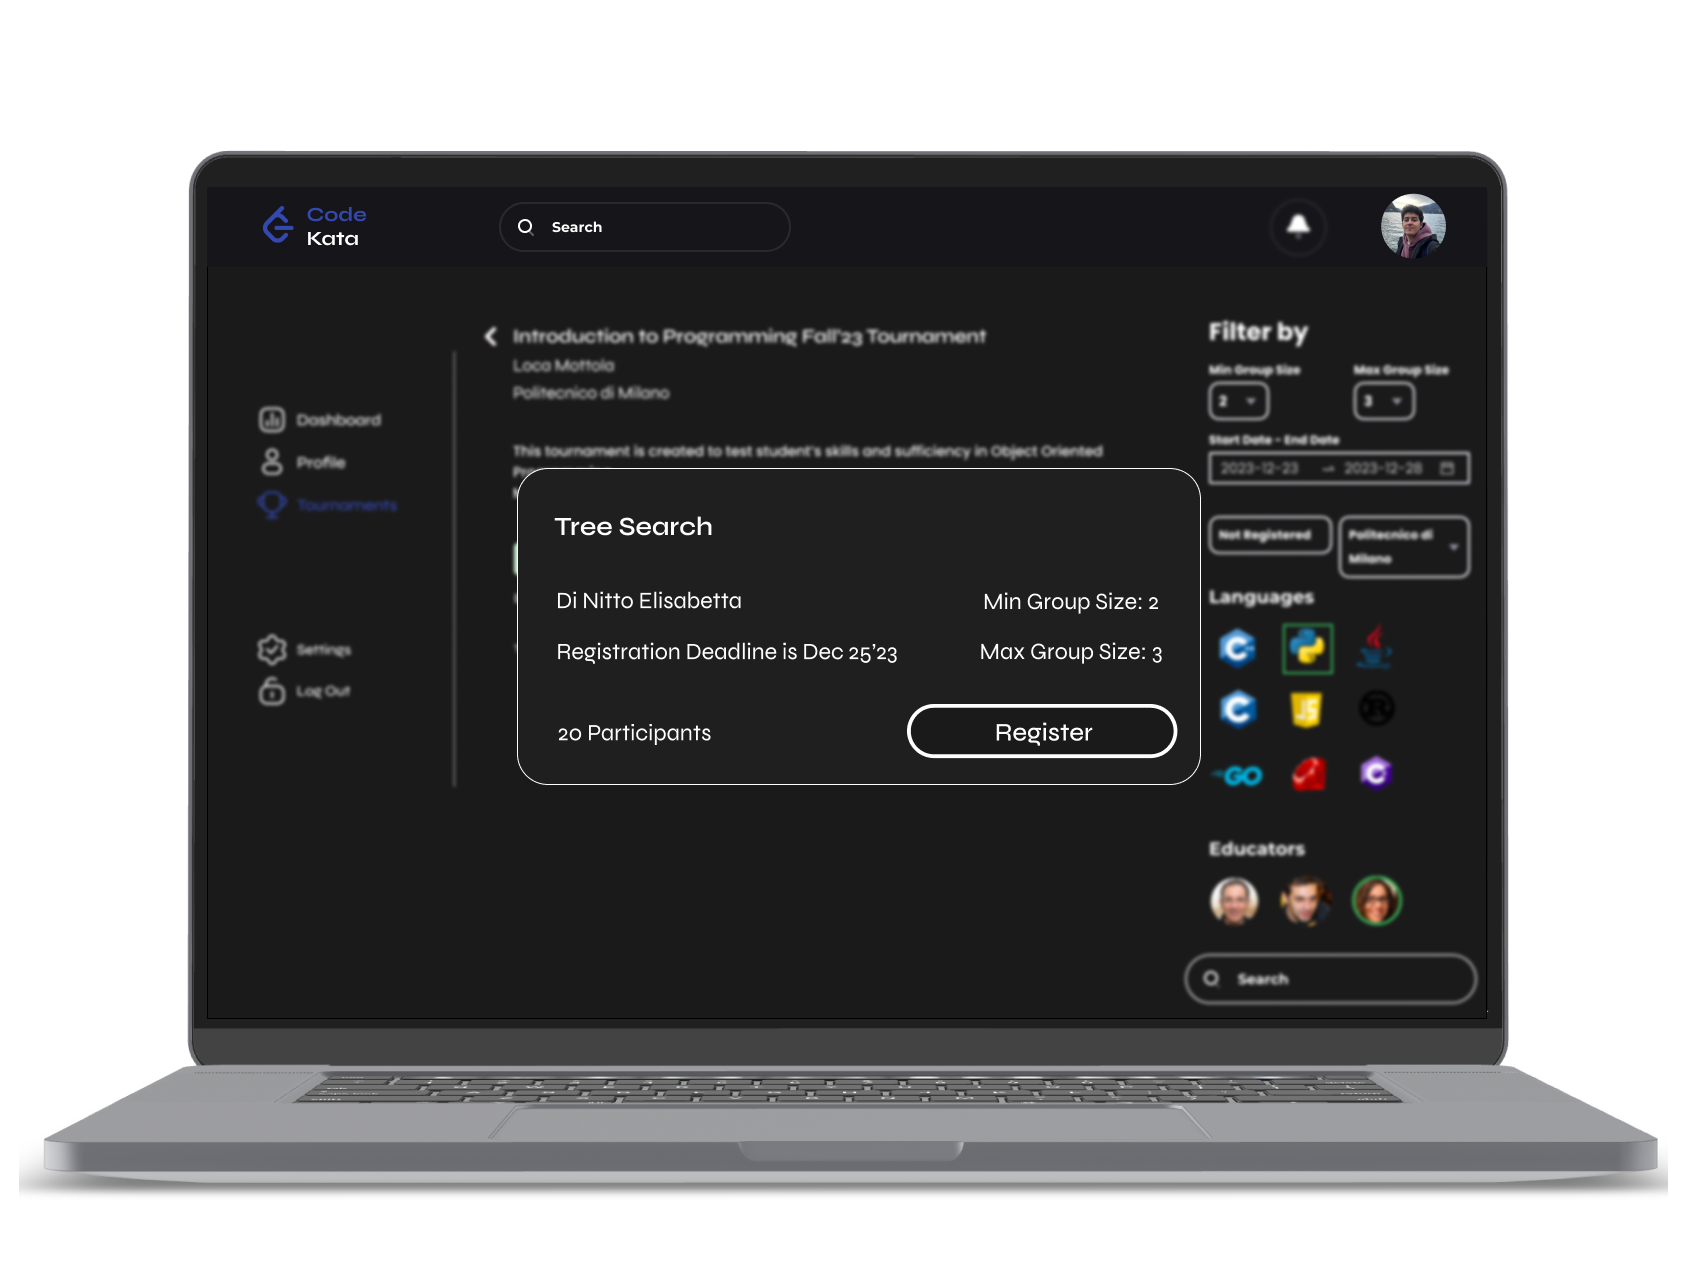
\includegraphics[scale=0.13]{Images/ui-ux/student_battle_register/student_battle_register_1.png}
% 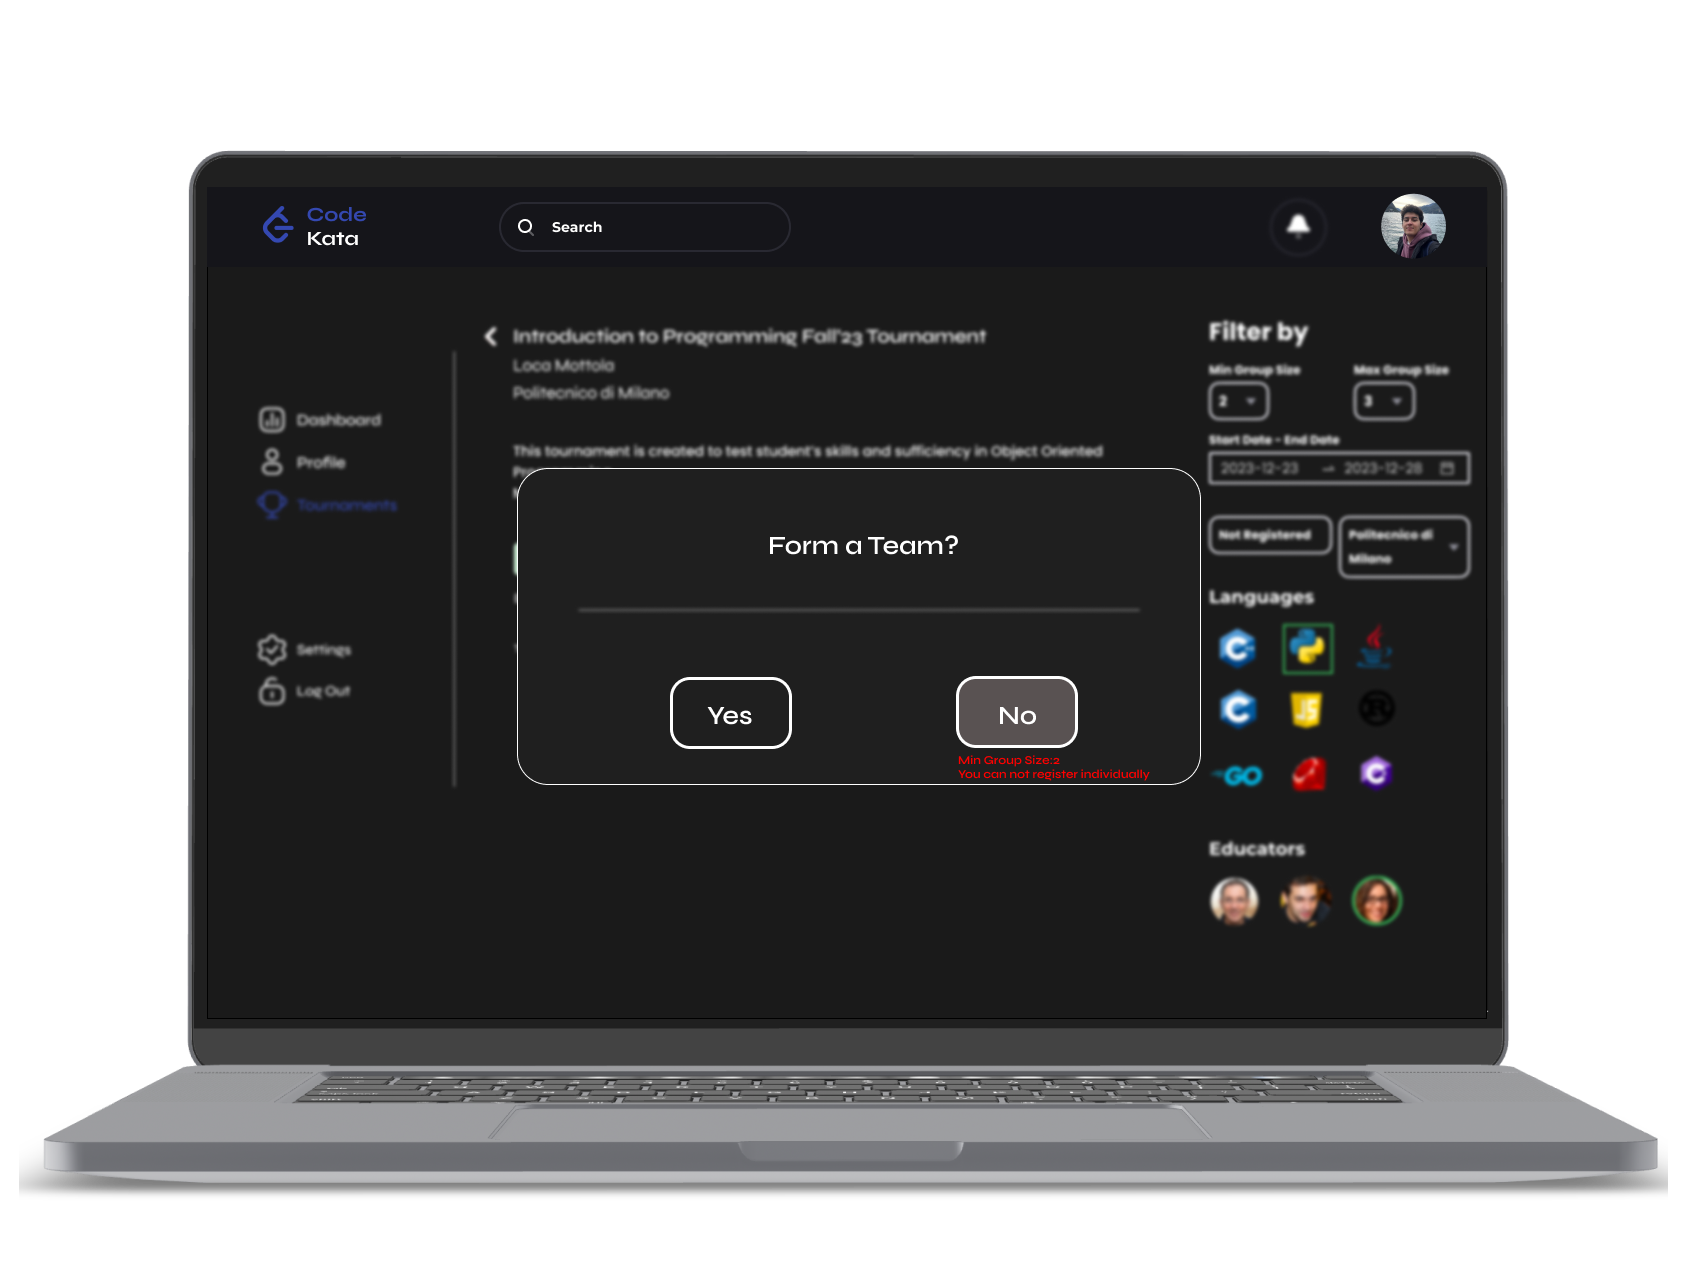
\includegraphics[scale=0.13]{Images/ui-ux/student_battle_register/student_battle_register_2.png}
% 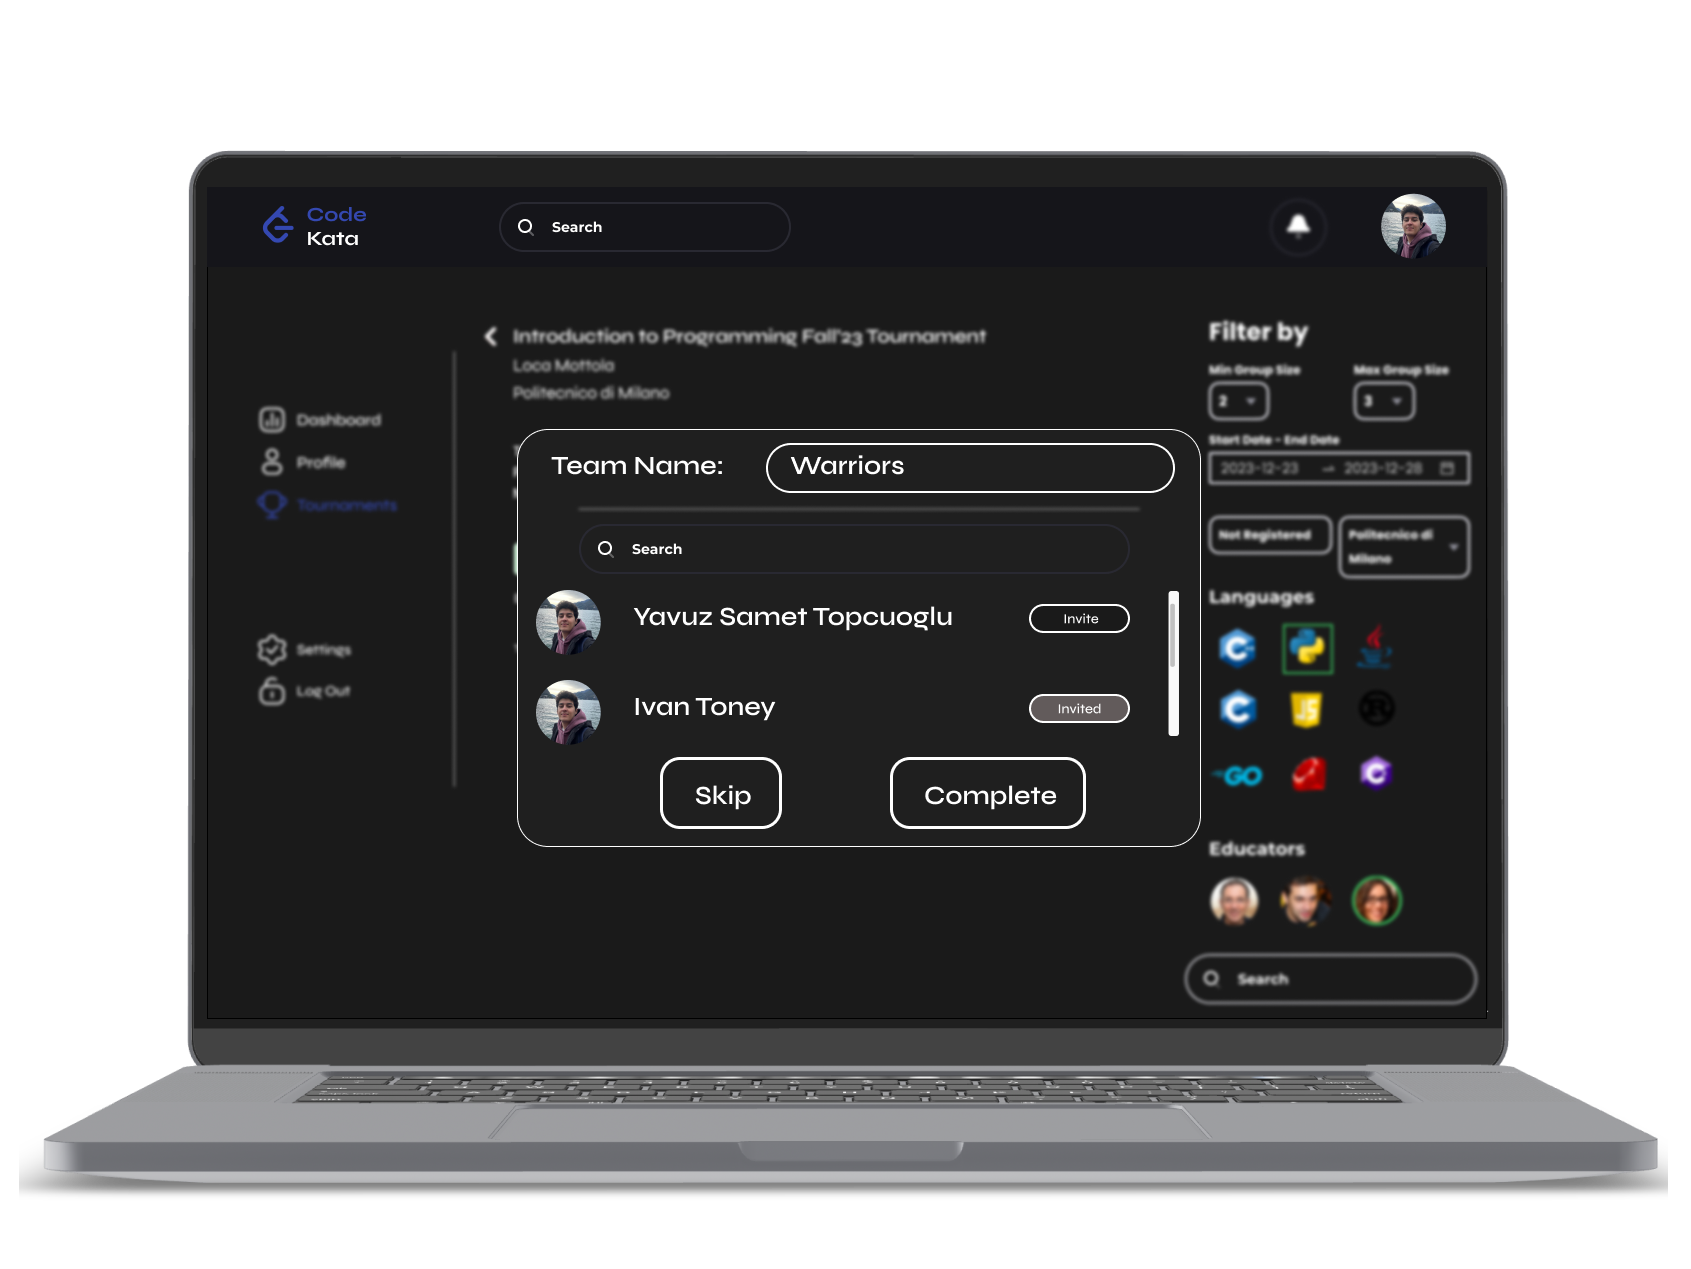
\includegraphics[scale=0.13]{Images/ui-ux/student_battle_register/student_battle_register_3.png}
% \\ (a) Student Registers Battle
% \end{center}
% \newpage
% \begin{center}
% 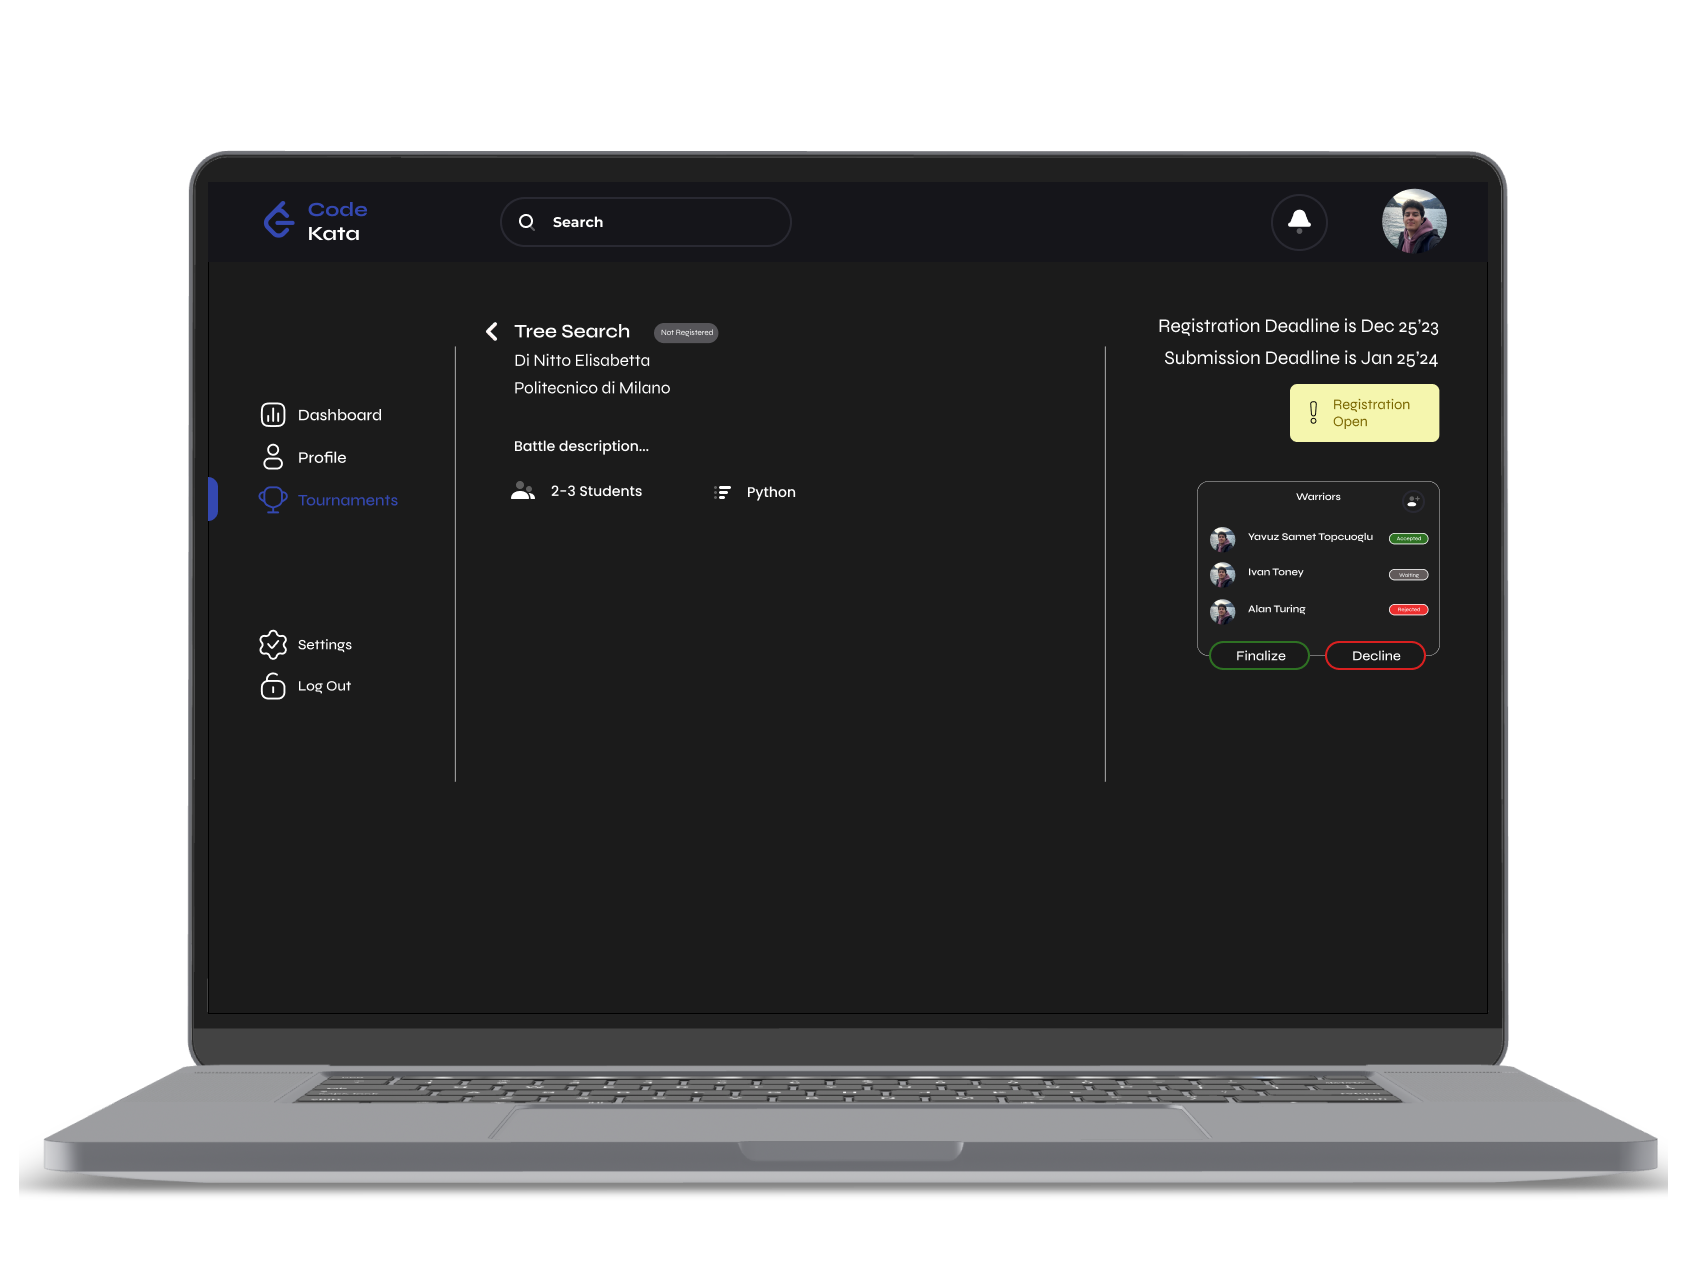
\includegraphics[scale=0.13]{Images/ui-ux/student_battle/student_battle_1.png}
% 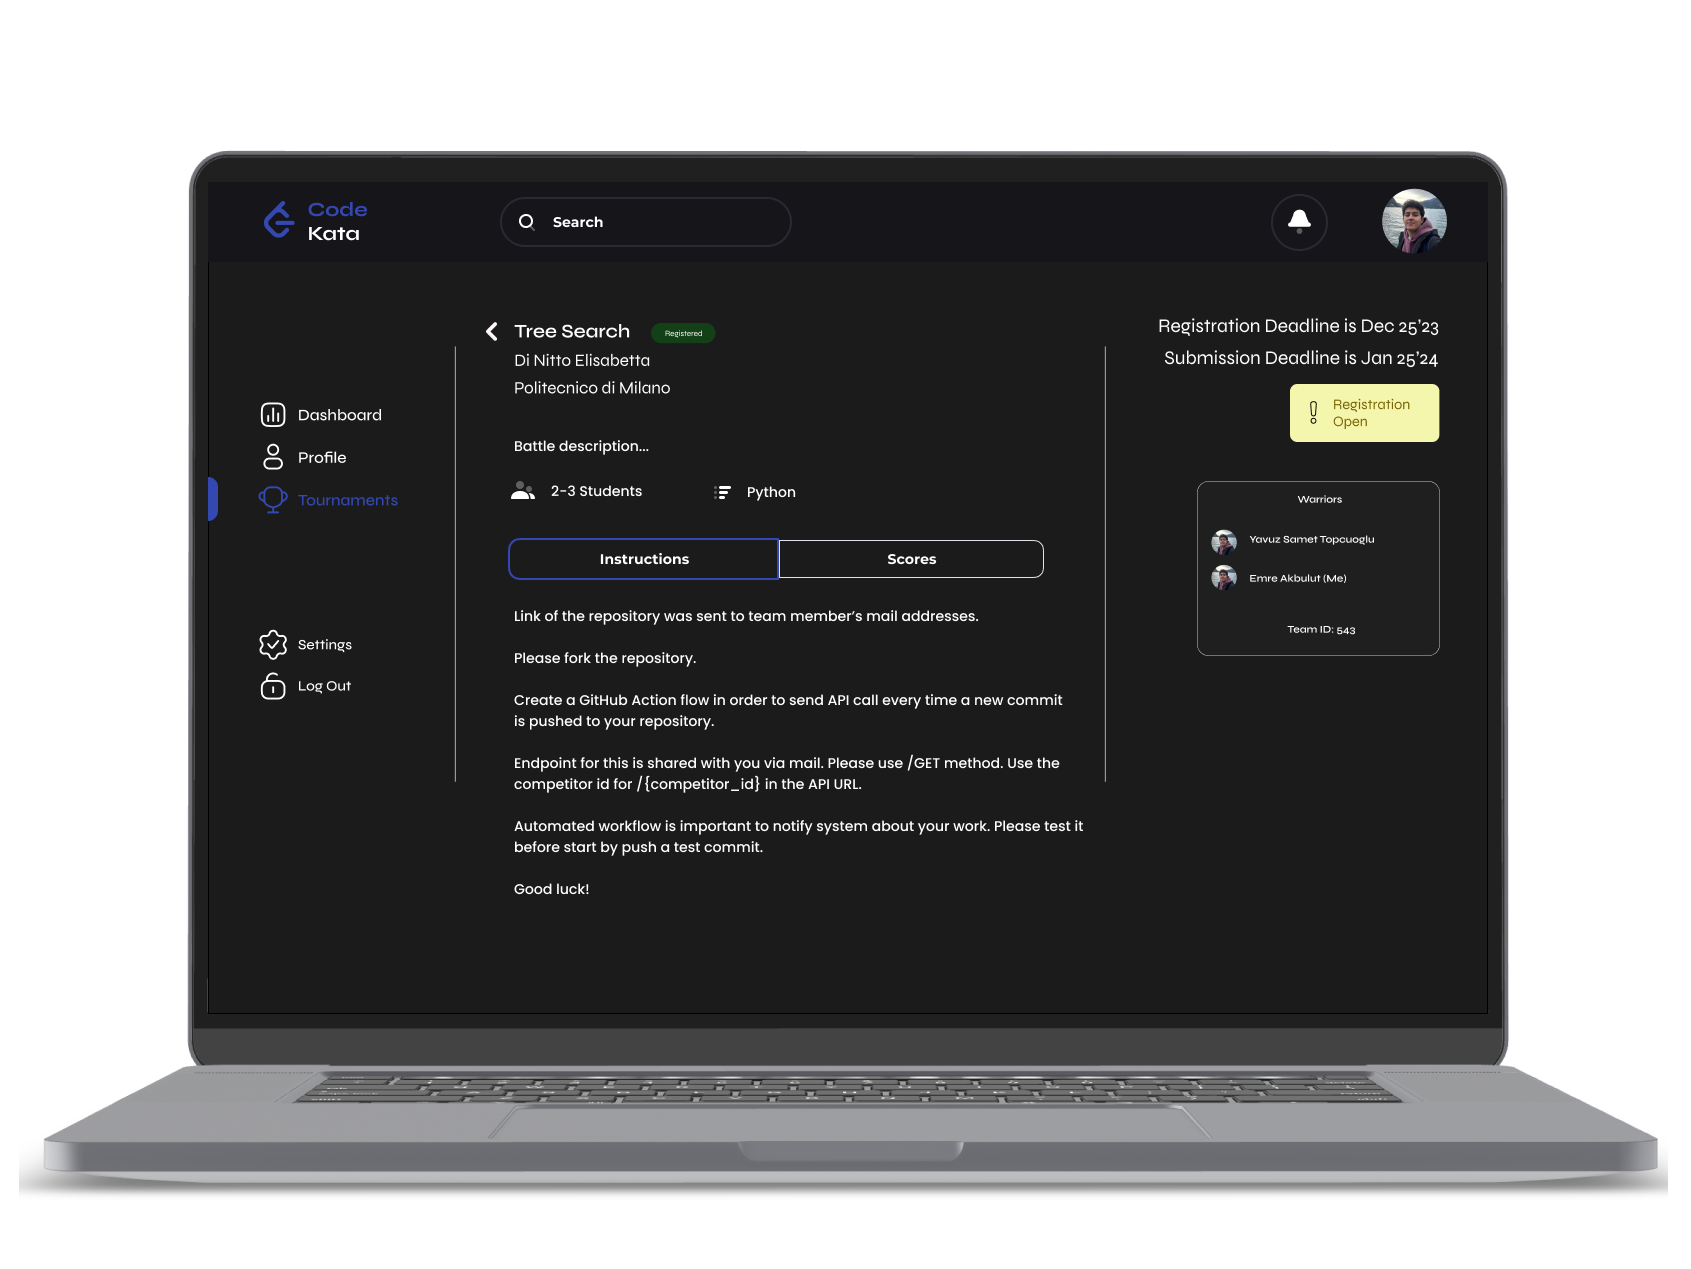
\includegraphics[scale=0.13]{Images/ui-ux/student_battle/student_battle_2.png}
% 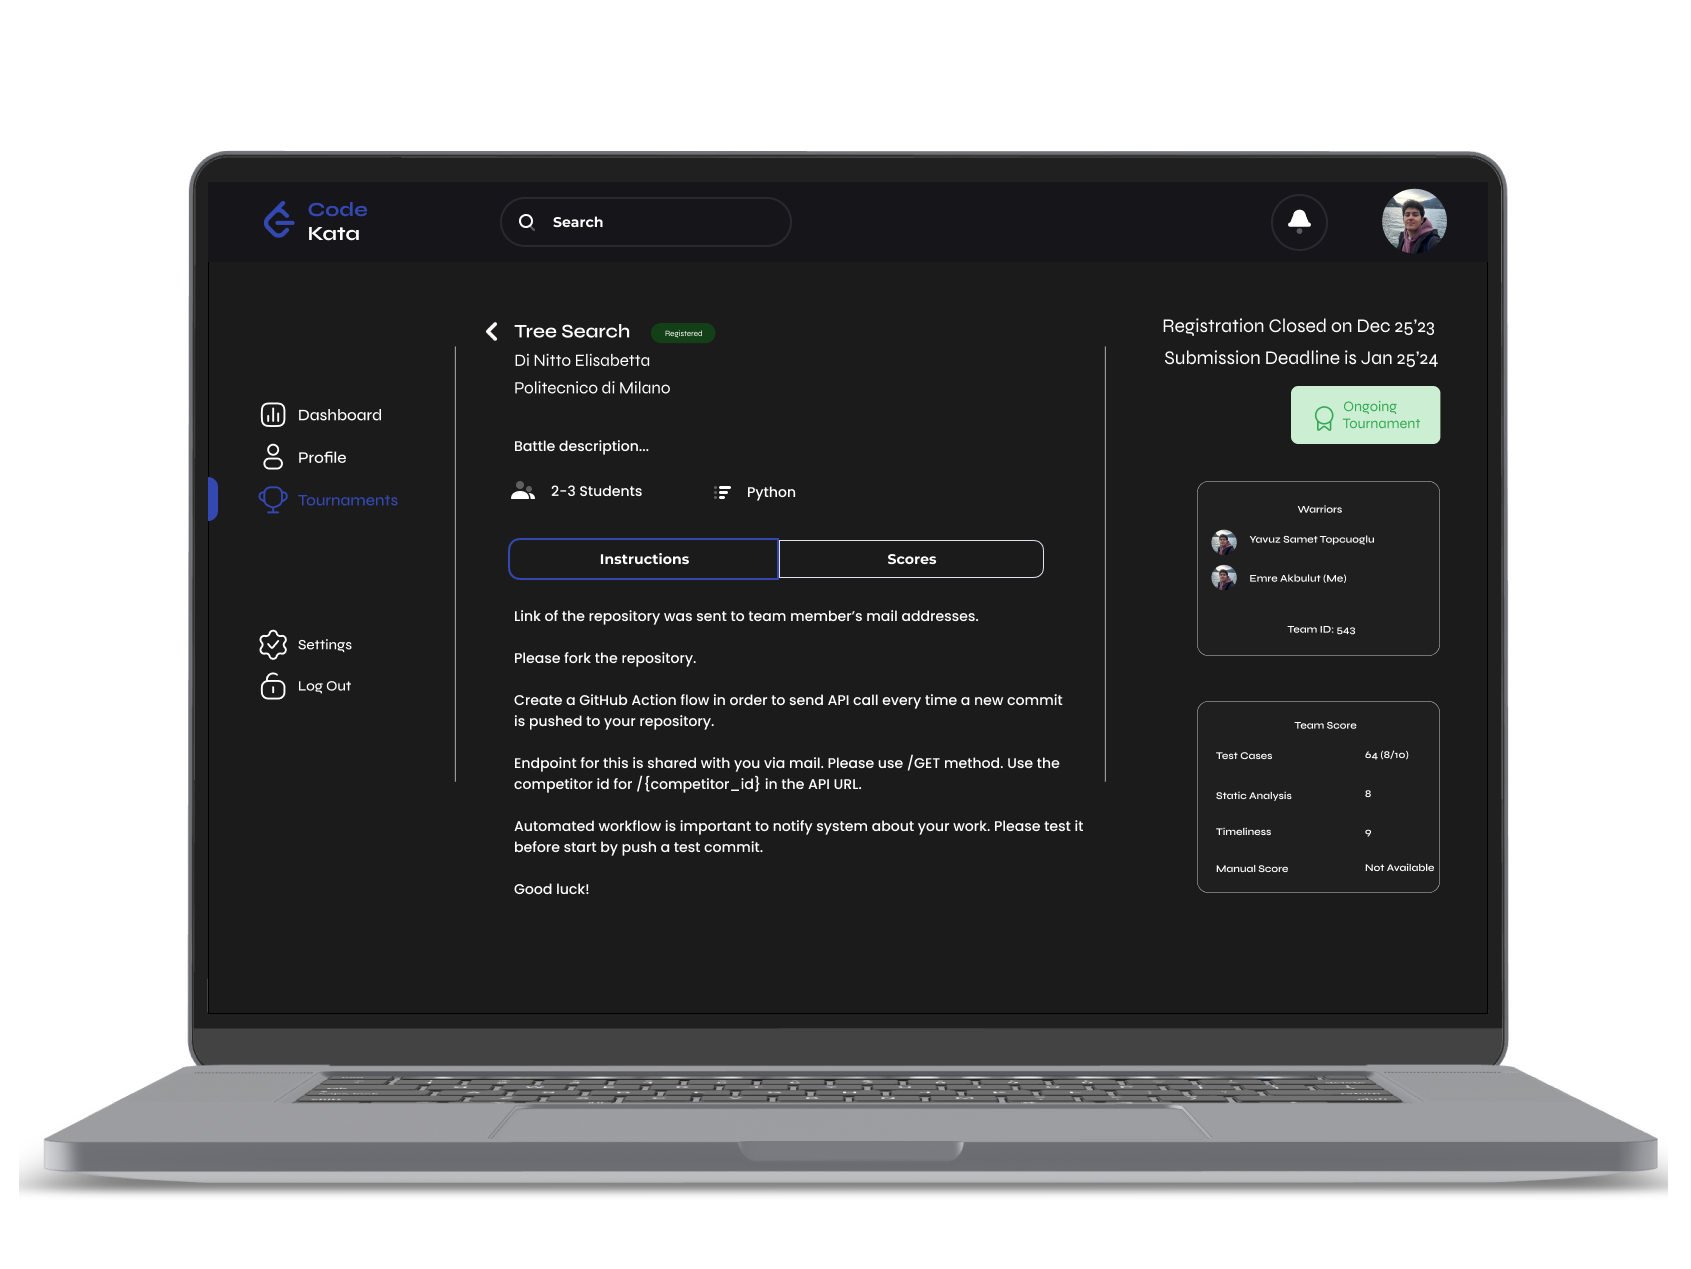
\includegraphics[scale=0.13]{Images/ui-ux/student_battle/student_battle_3.png}
% 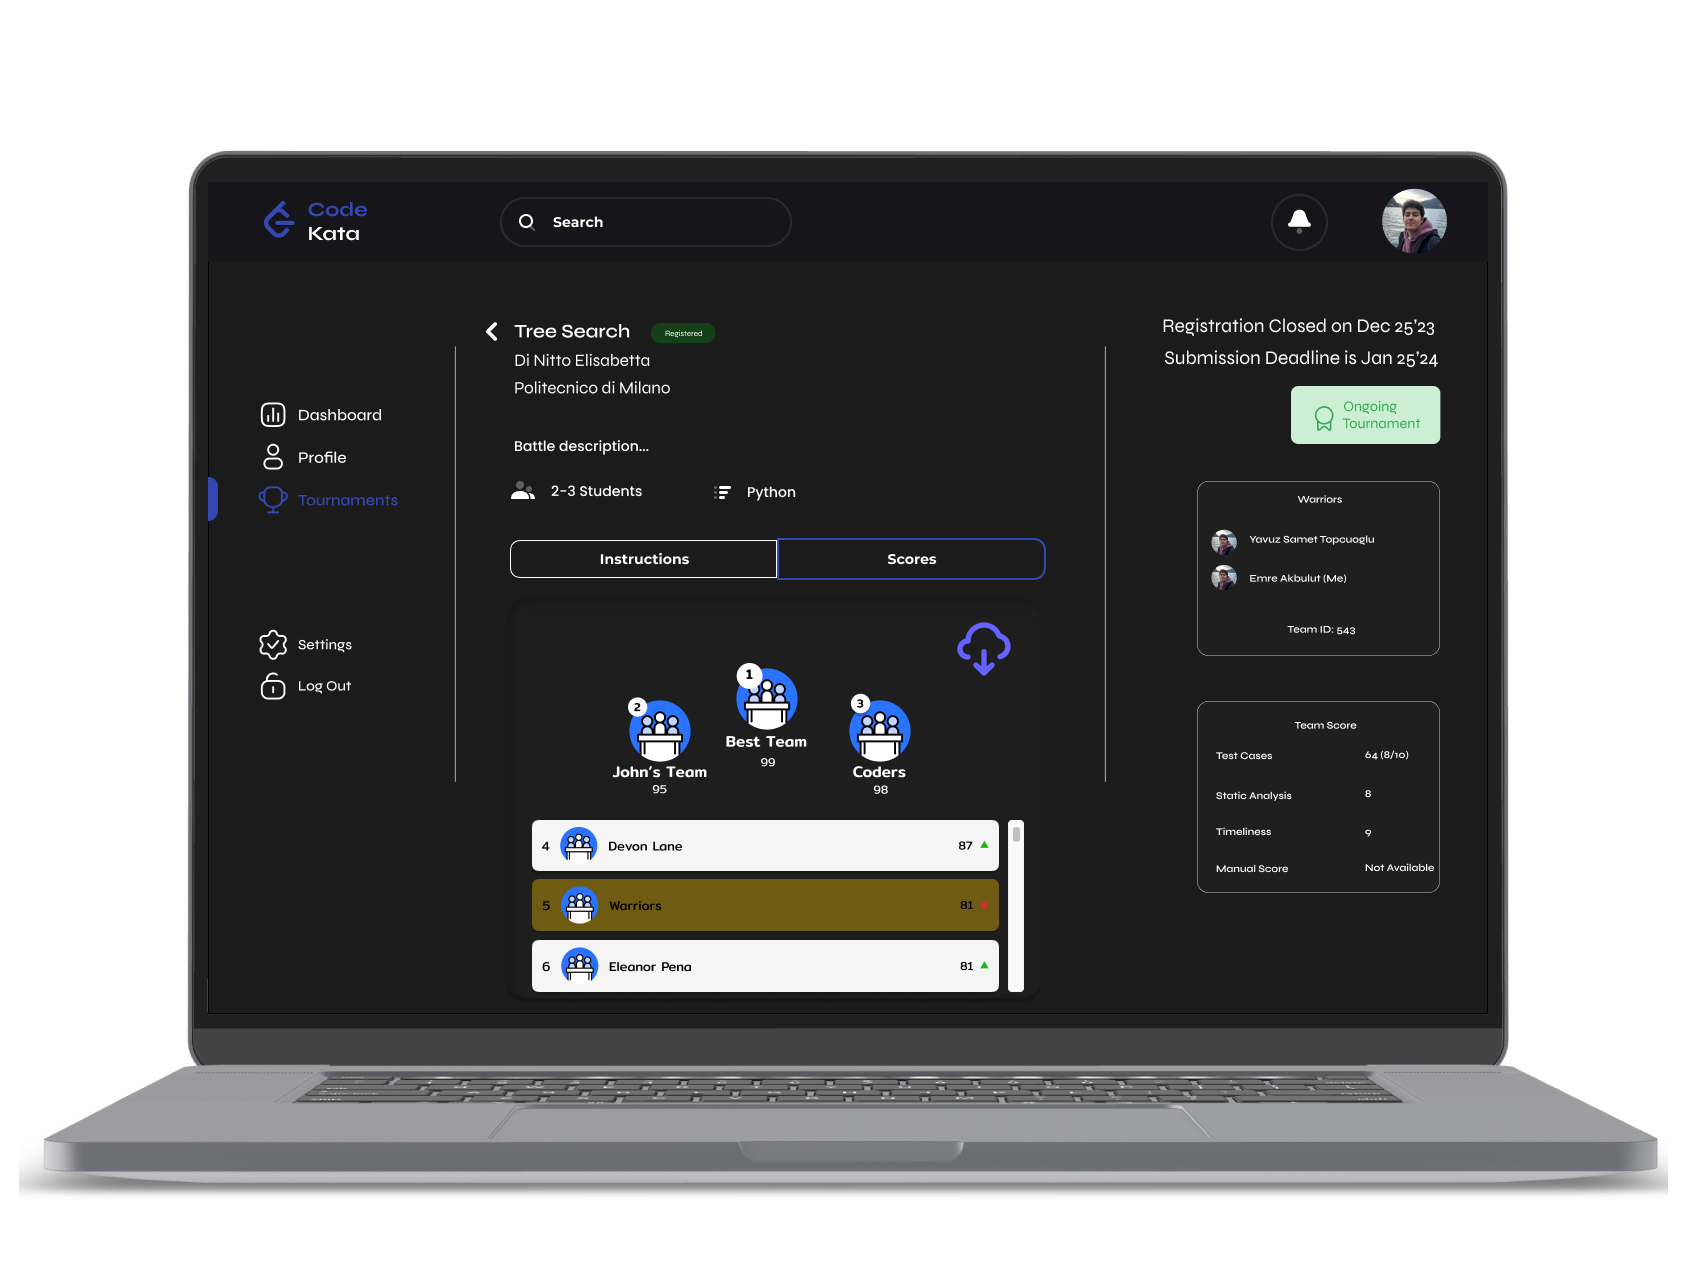
\includegraphics[scale=0.13]{Images/ui-ux/student_battle/student_battle_4.png}
%       (a) Battle Screen for Student
% \end{center}

% \begin{center}
% 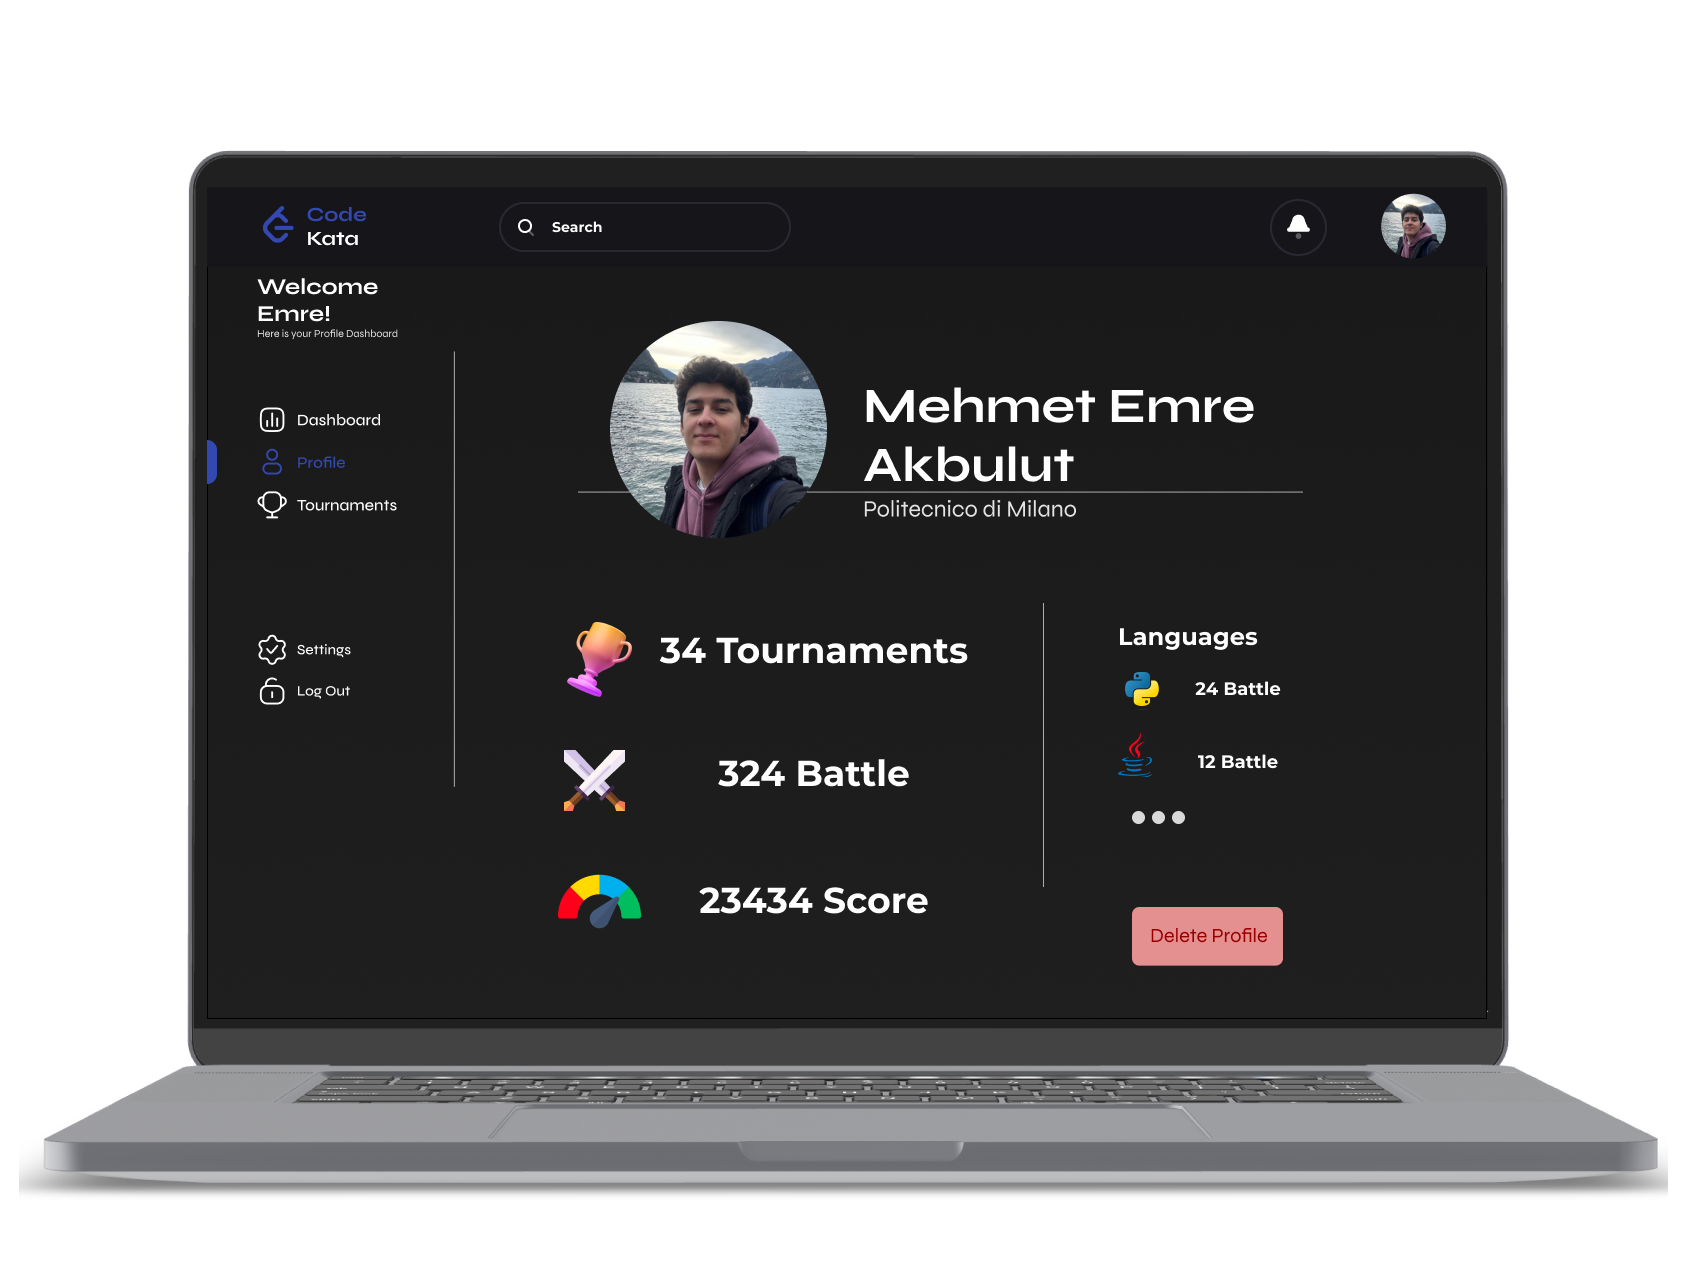
\includegraphics[scale=0.13]{Images/ui-ux/student_profile_settings/student_profile.png}
% 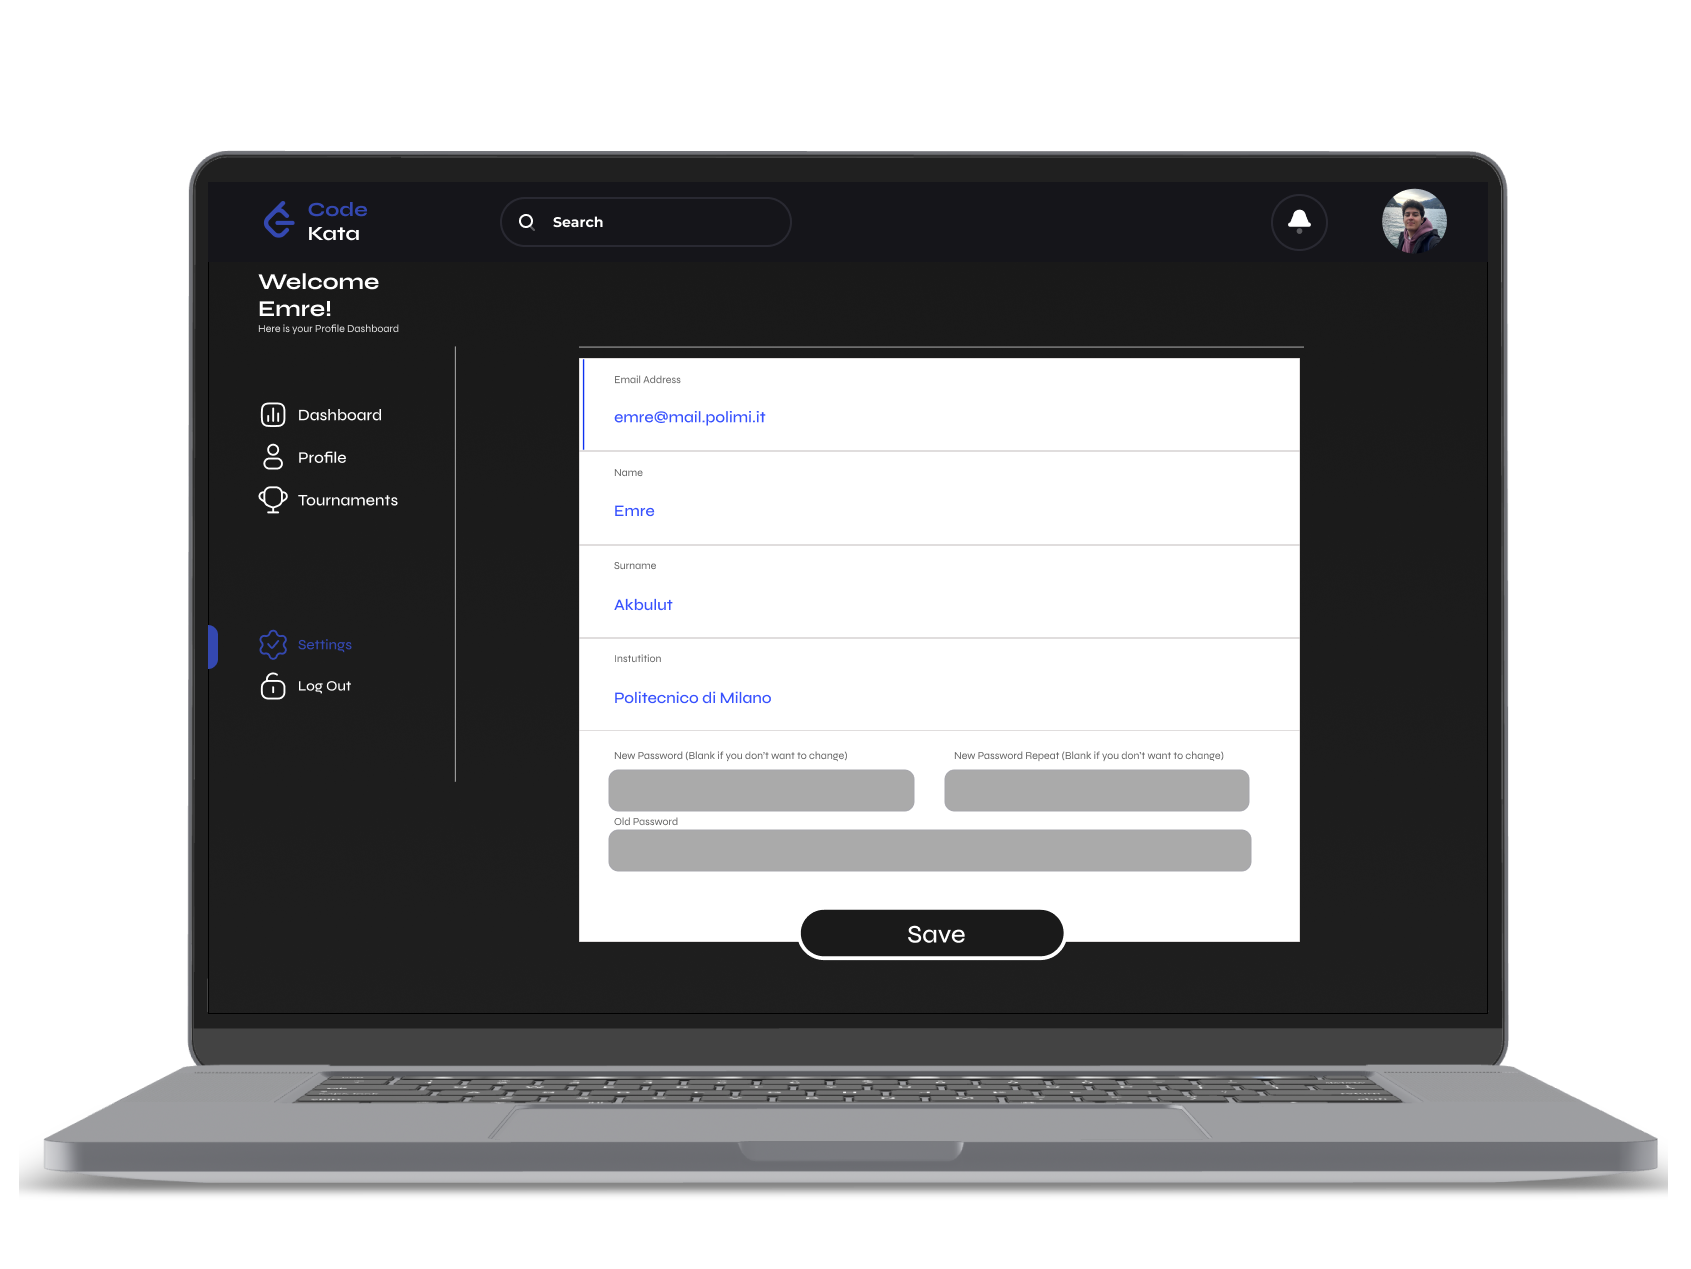
\includegraphics[scale=0.13]{Images/ui-ux/student_profile_settings/student_settings.png}
%         (a) Profile and Settings for Student
% \end{center}
% \newpage
% \begin{center}
% 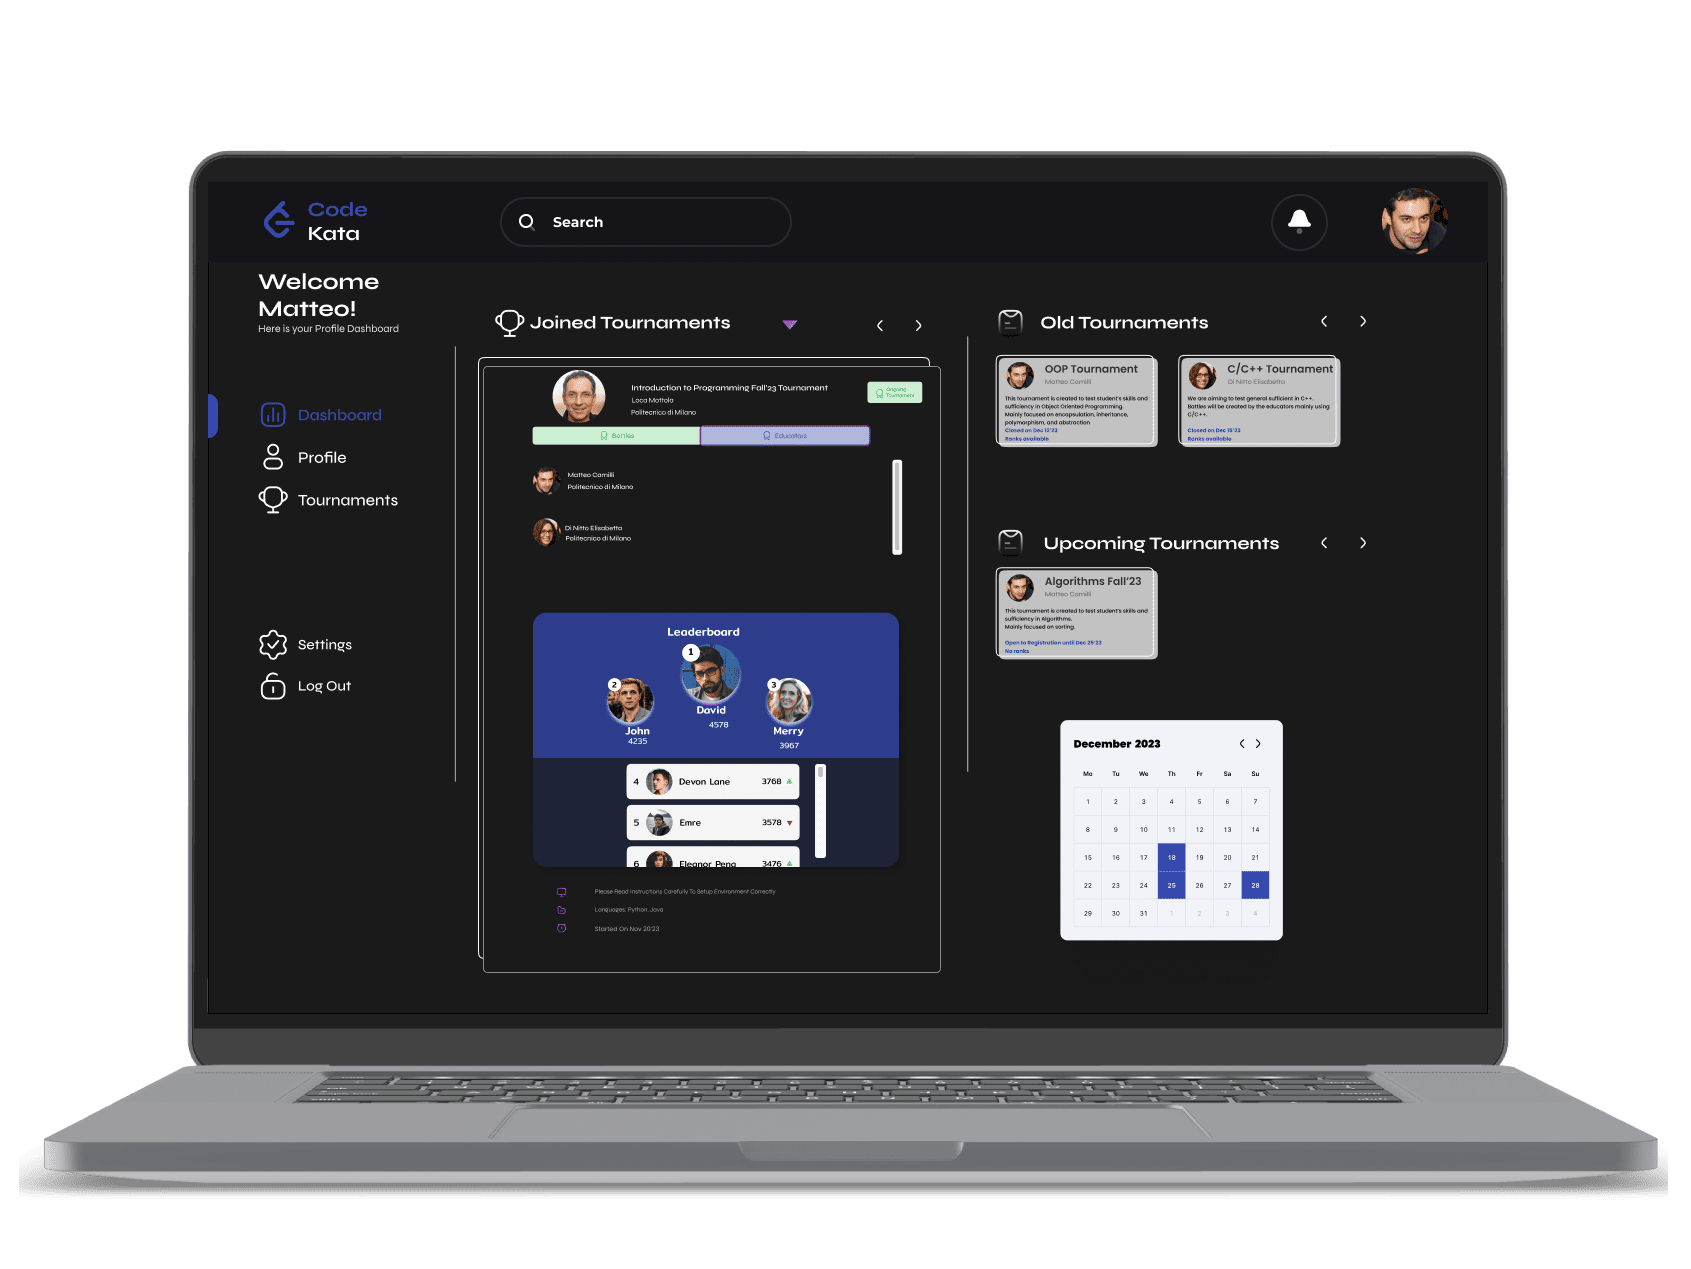
\includegraphics[scale=0.13]{Images/ui-ux/educator_dashboard/educator_dashboard_1.png}
% 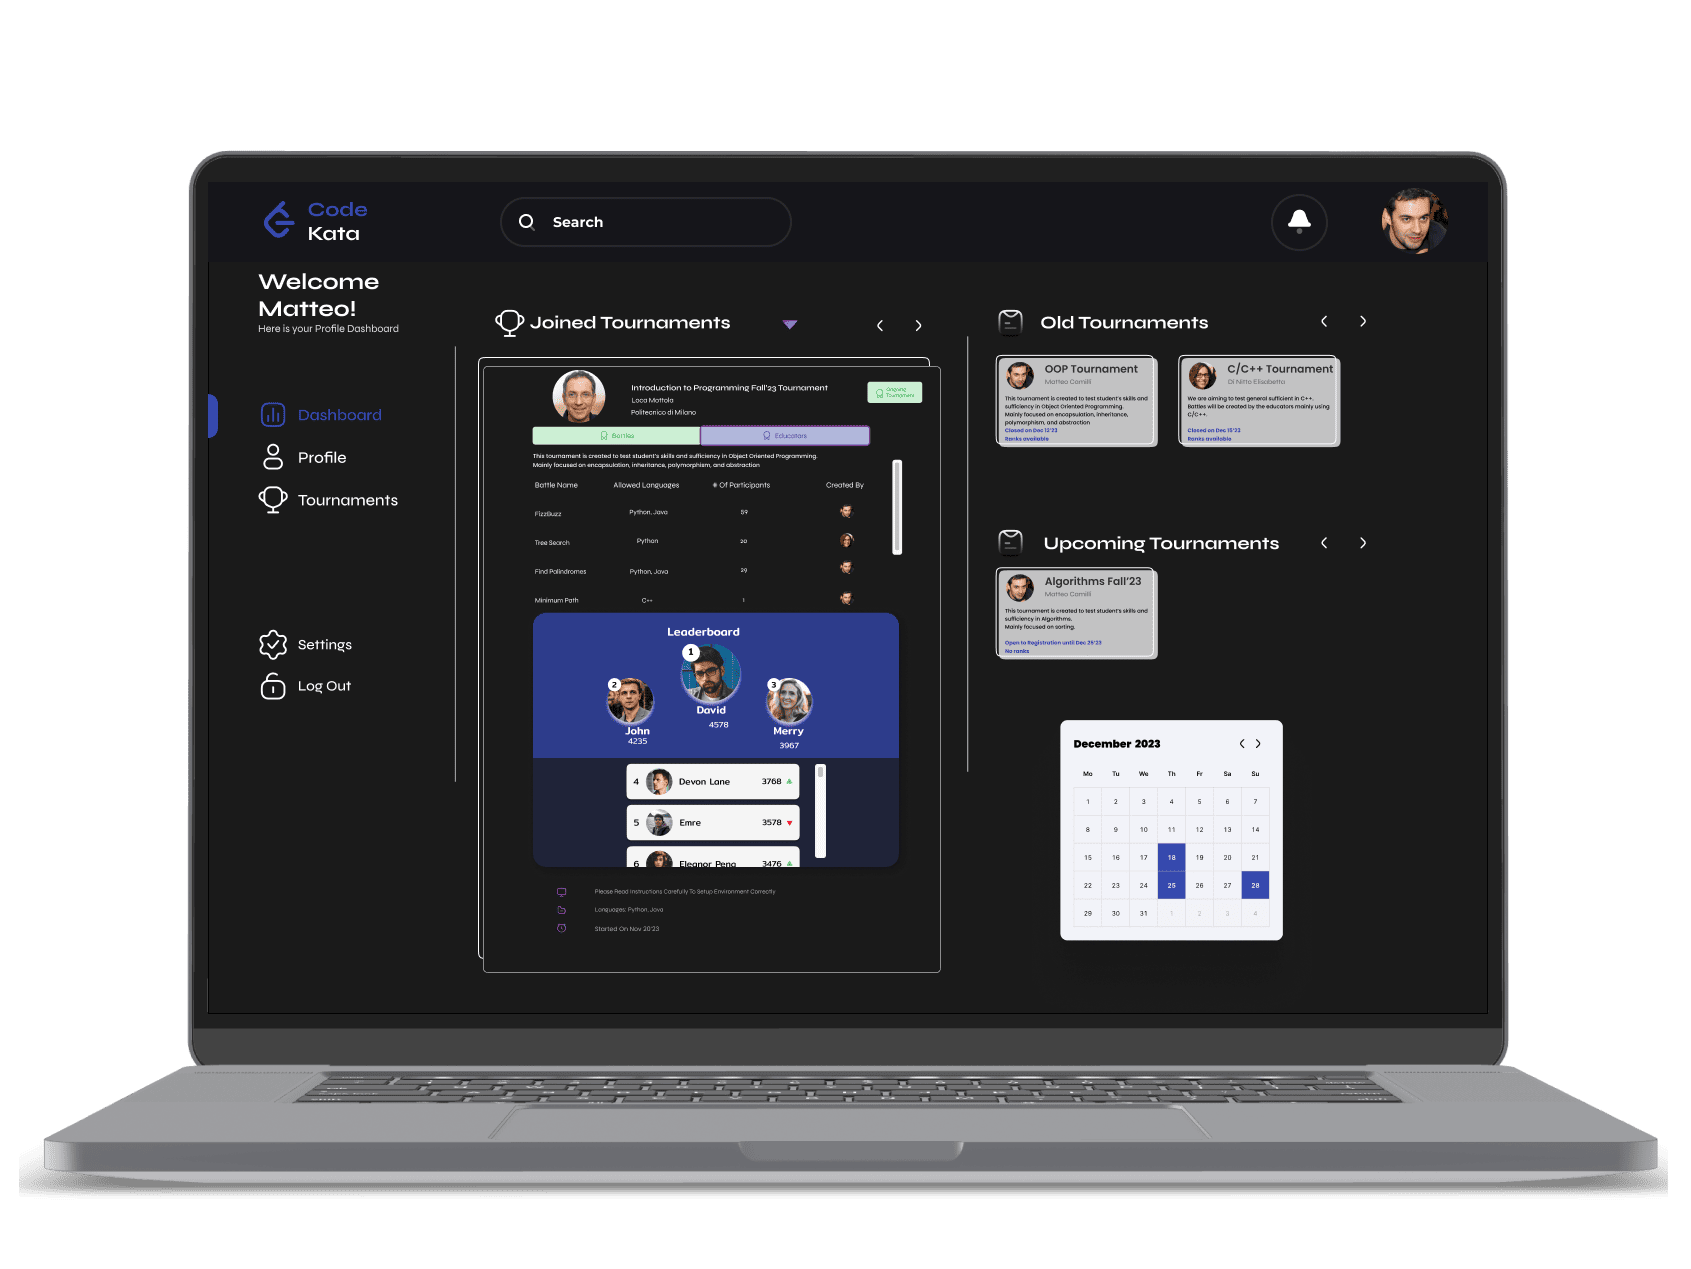
\includegraphics[scale=0.13]{Images/ui-ux/educator_dashboard/educator_dashboard_2.png}
% 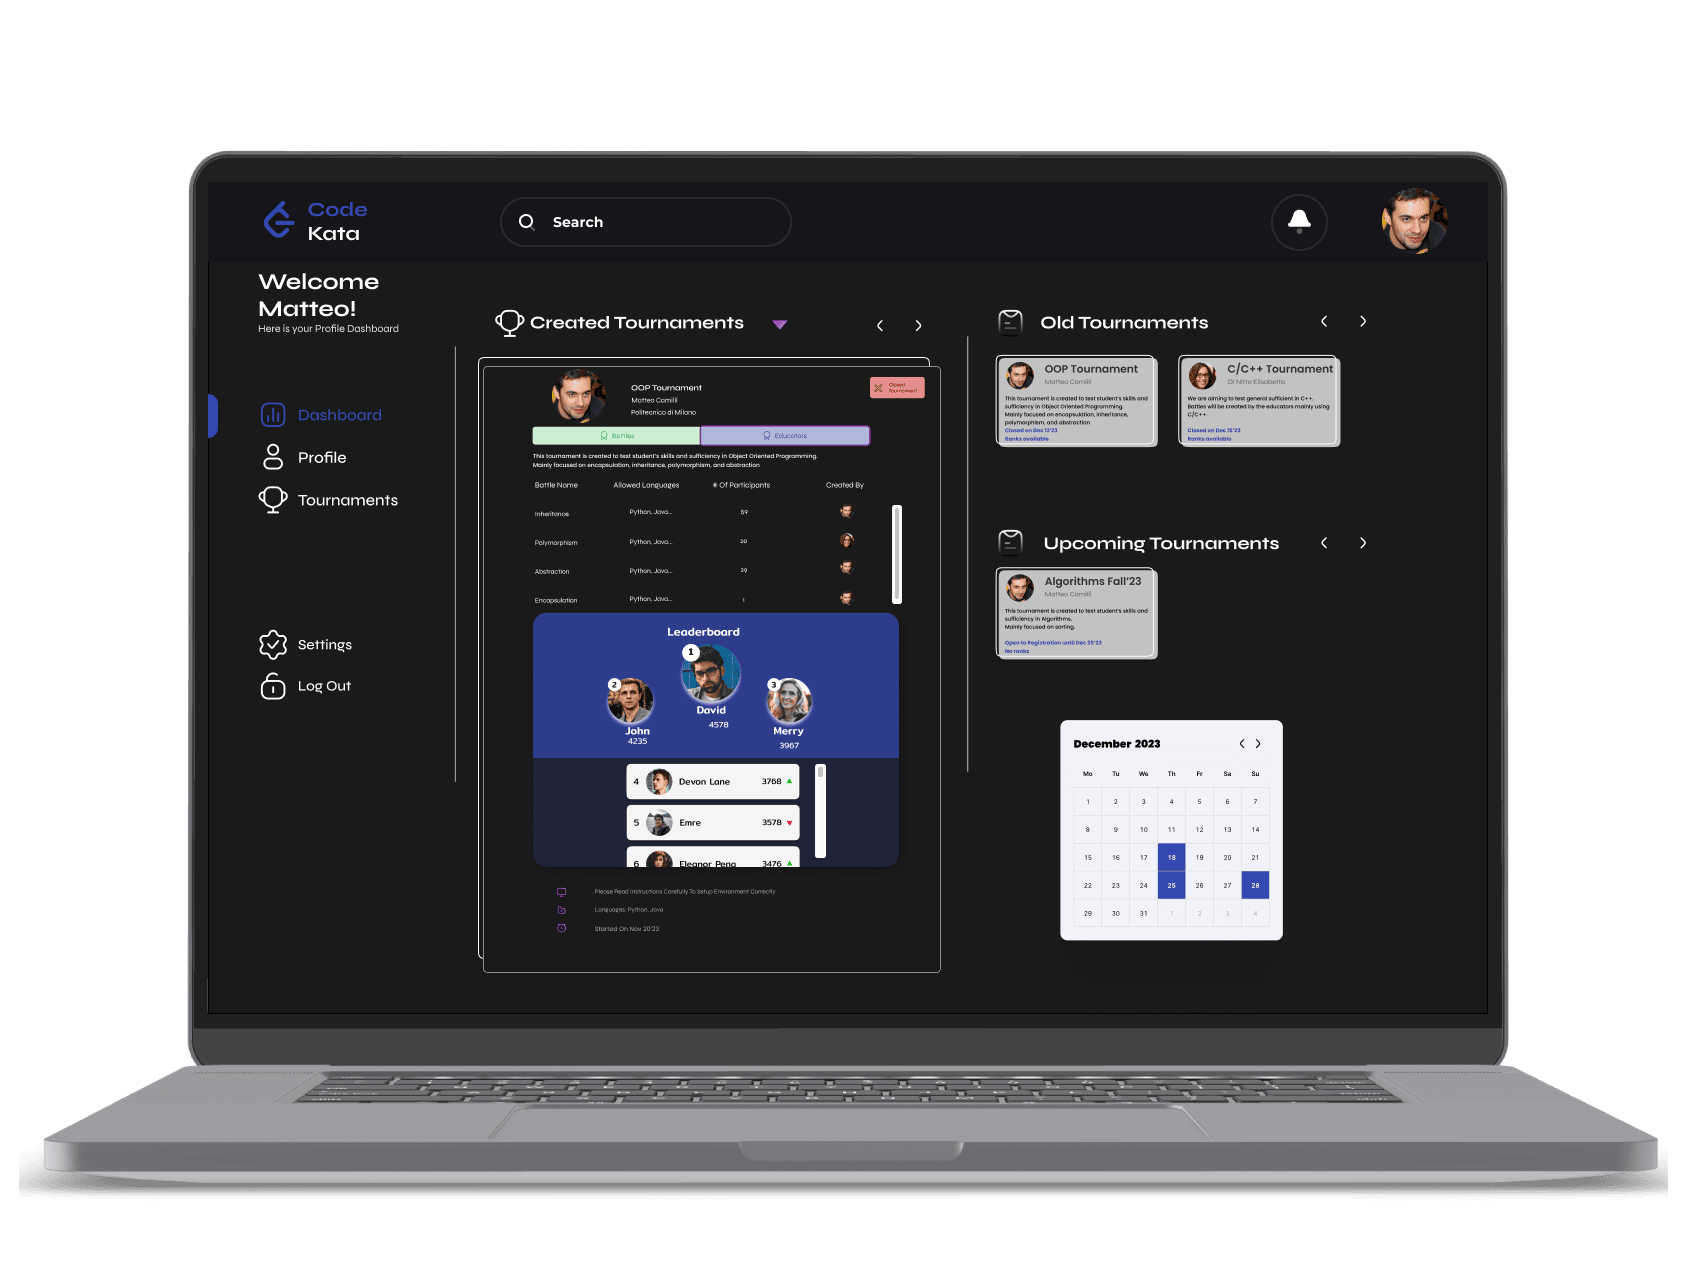
\includegraphics[scale=0.13]{Images/ui-ux/educator_dashboard/educator_dashboard_3.png}
% \\ (a) Educator Dashboard
% \end{center}
% \begin{center}
% 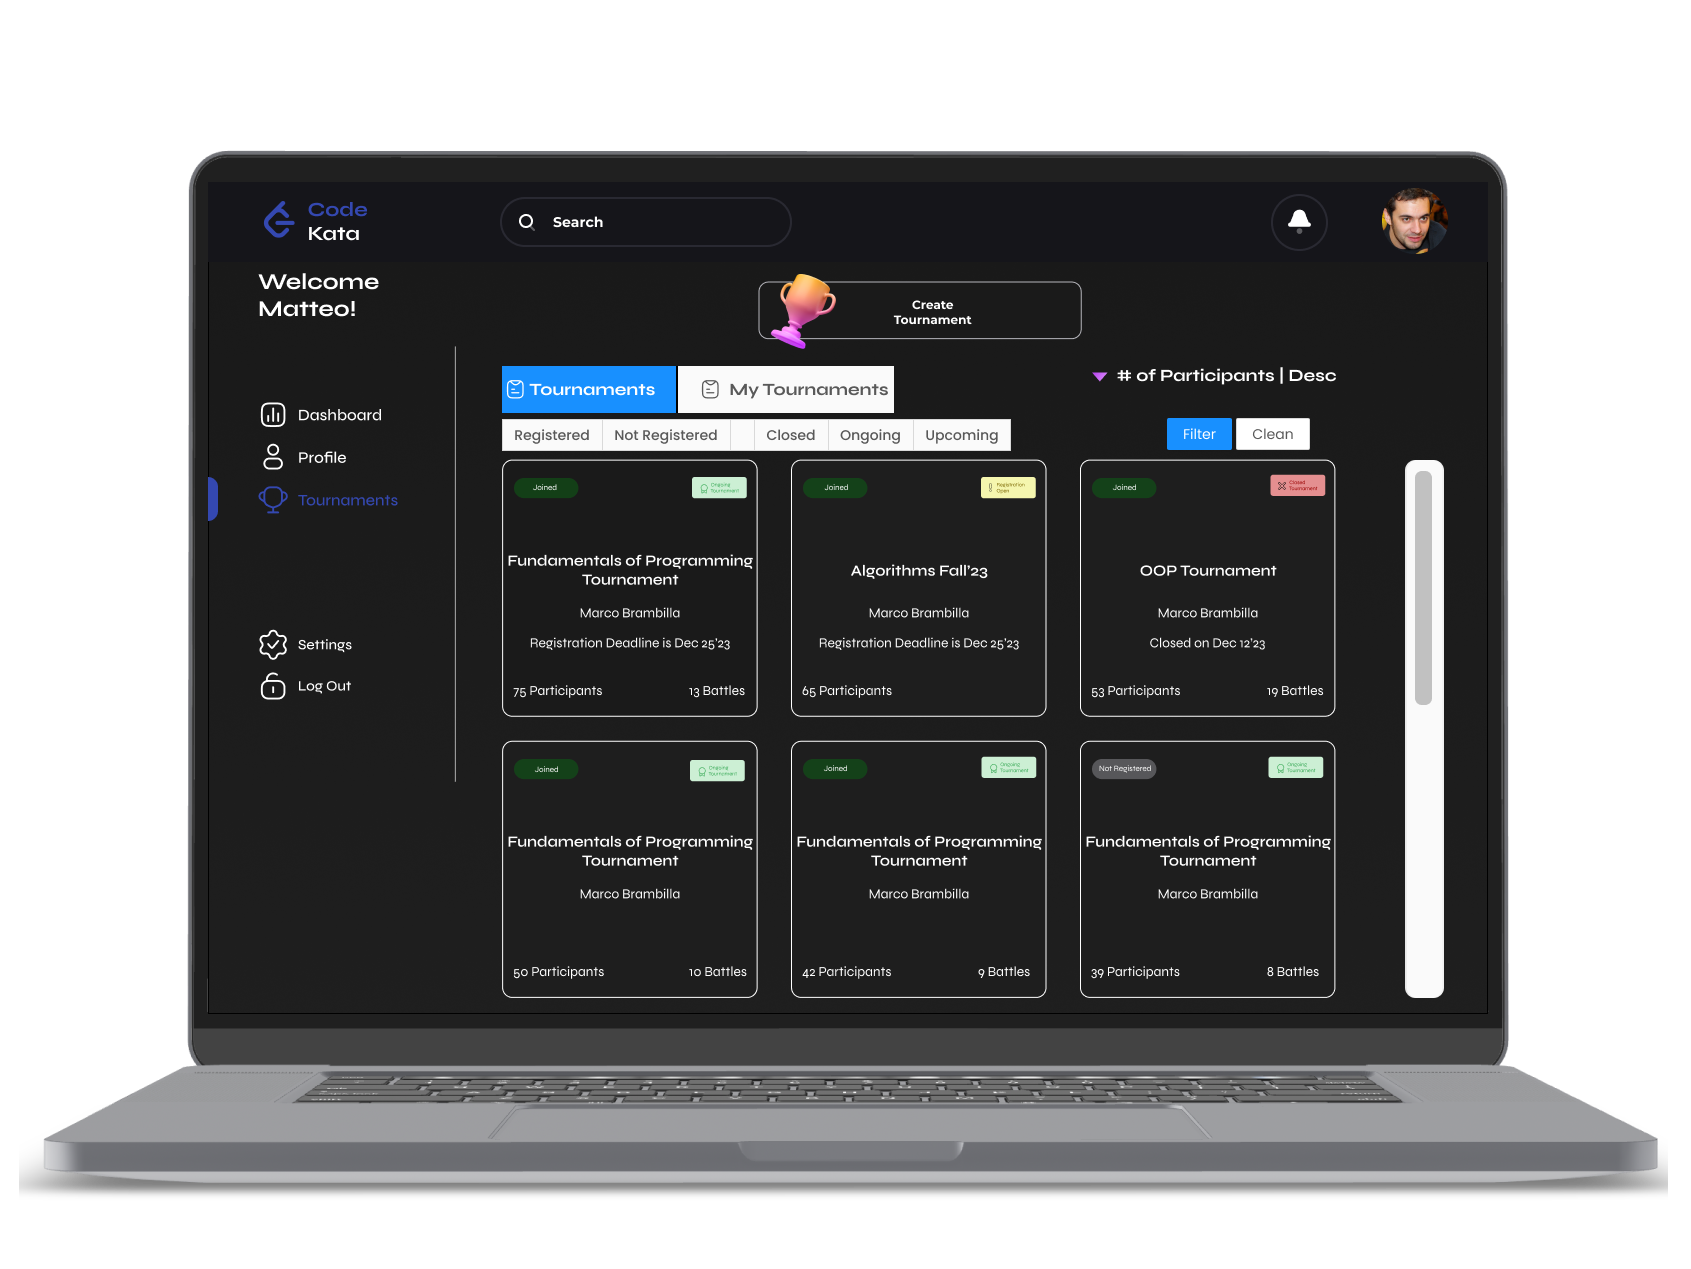
\includegraphics[scale=0.13]{Images/ui-ux/educator_tournaments/educator_tournaments_1.png}
% 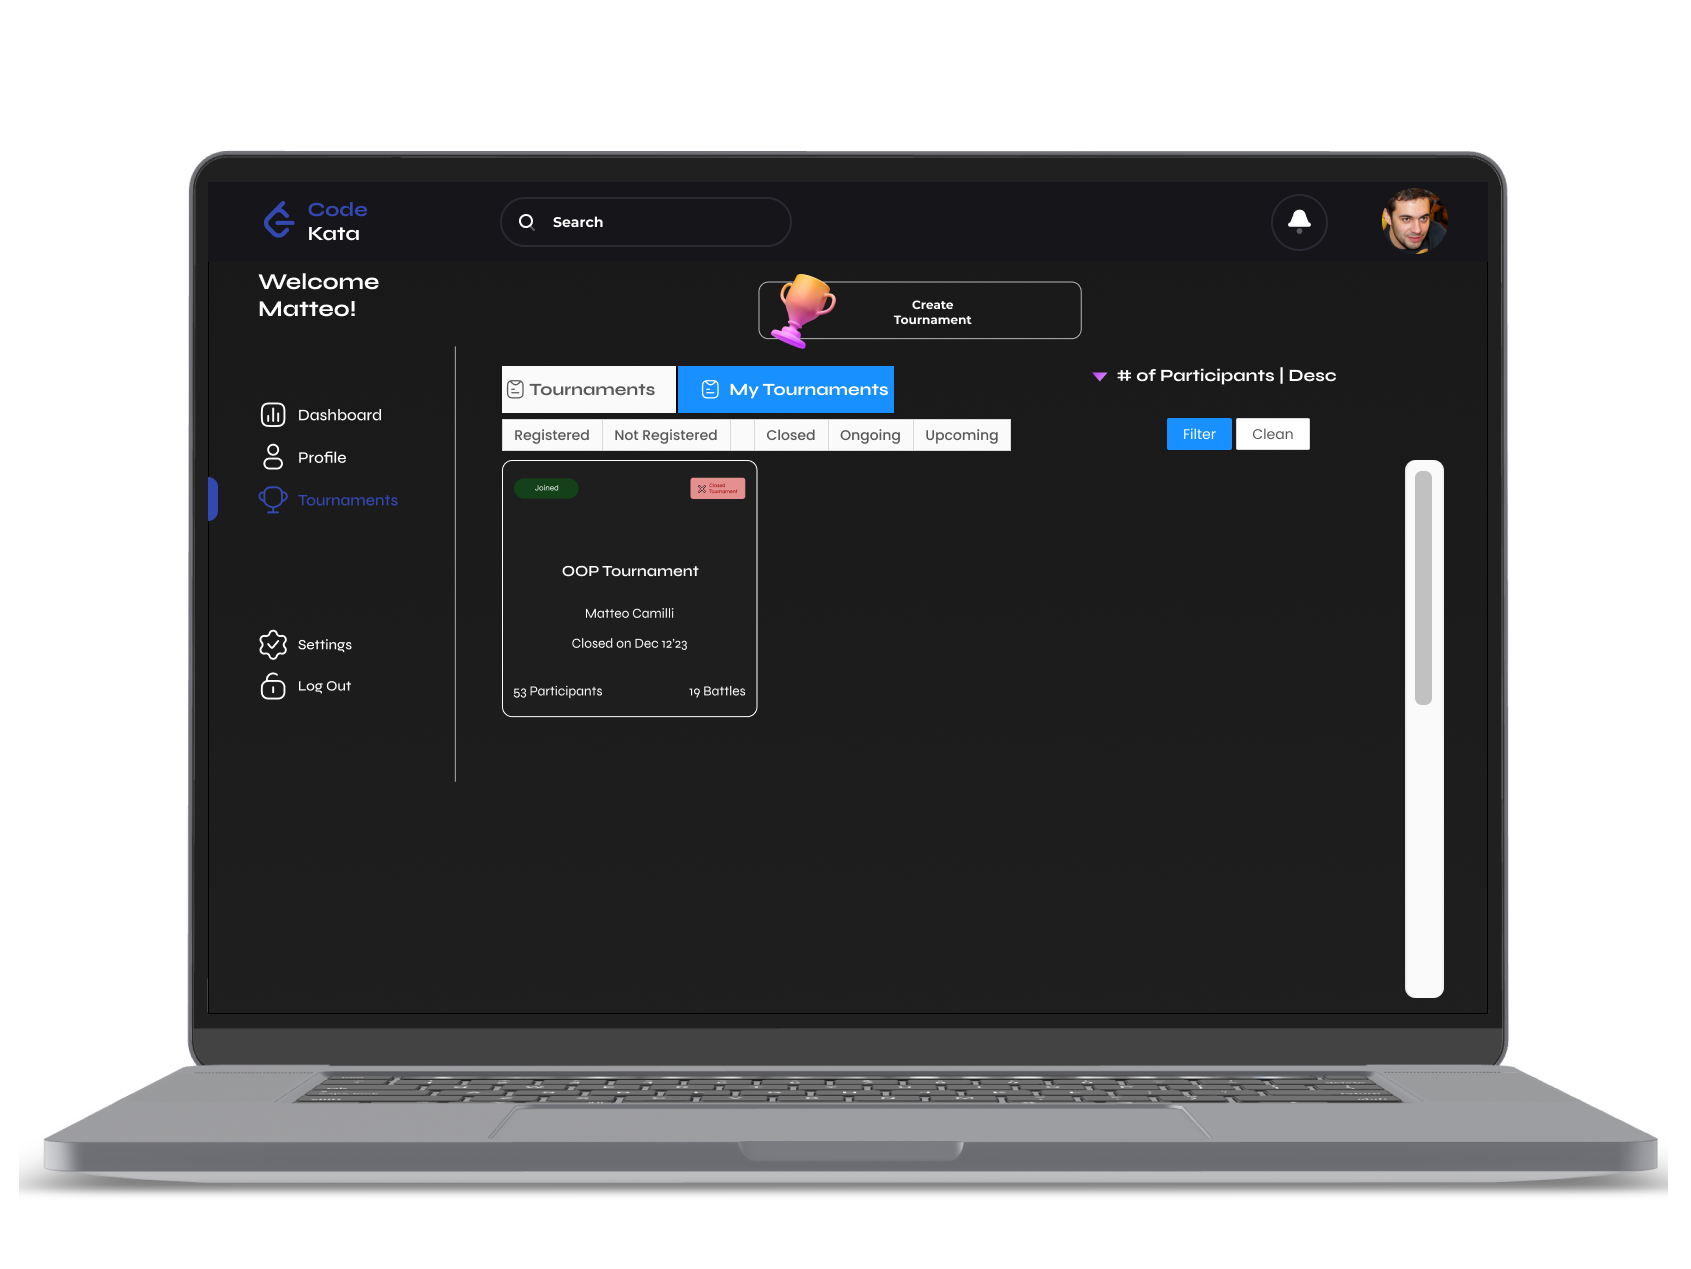
\includegraphics[scale=0.13]{Images/ui-ux/educator_tournaments/educator_tournaments_2.png}
%         (a) Educator Tournaments
% \end{center}
% \begin{center}
% 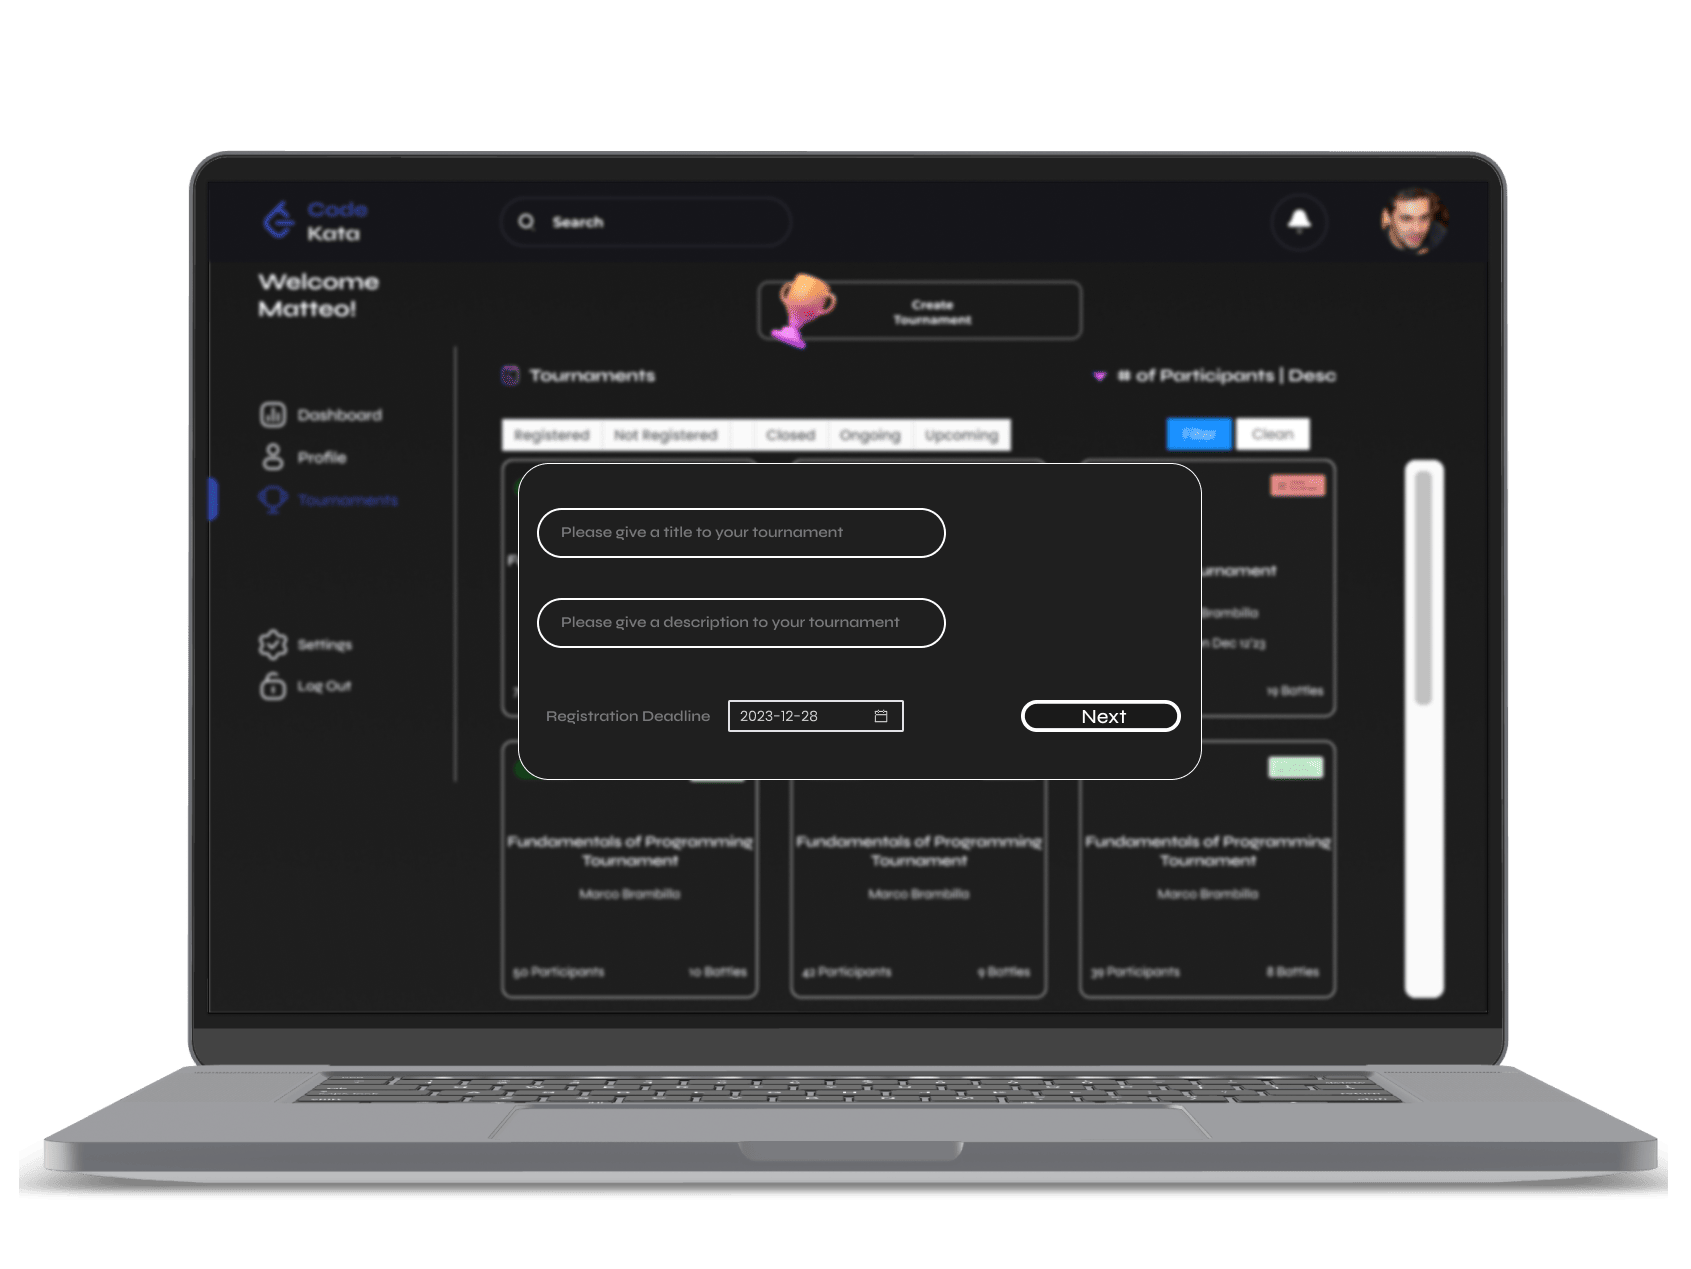
\includegraphics[scale=0.13]{Images/ui-ux/educator_create_tournament/educator_create_tournament_1.png}
% 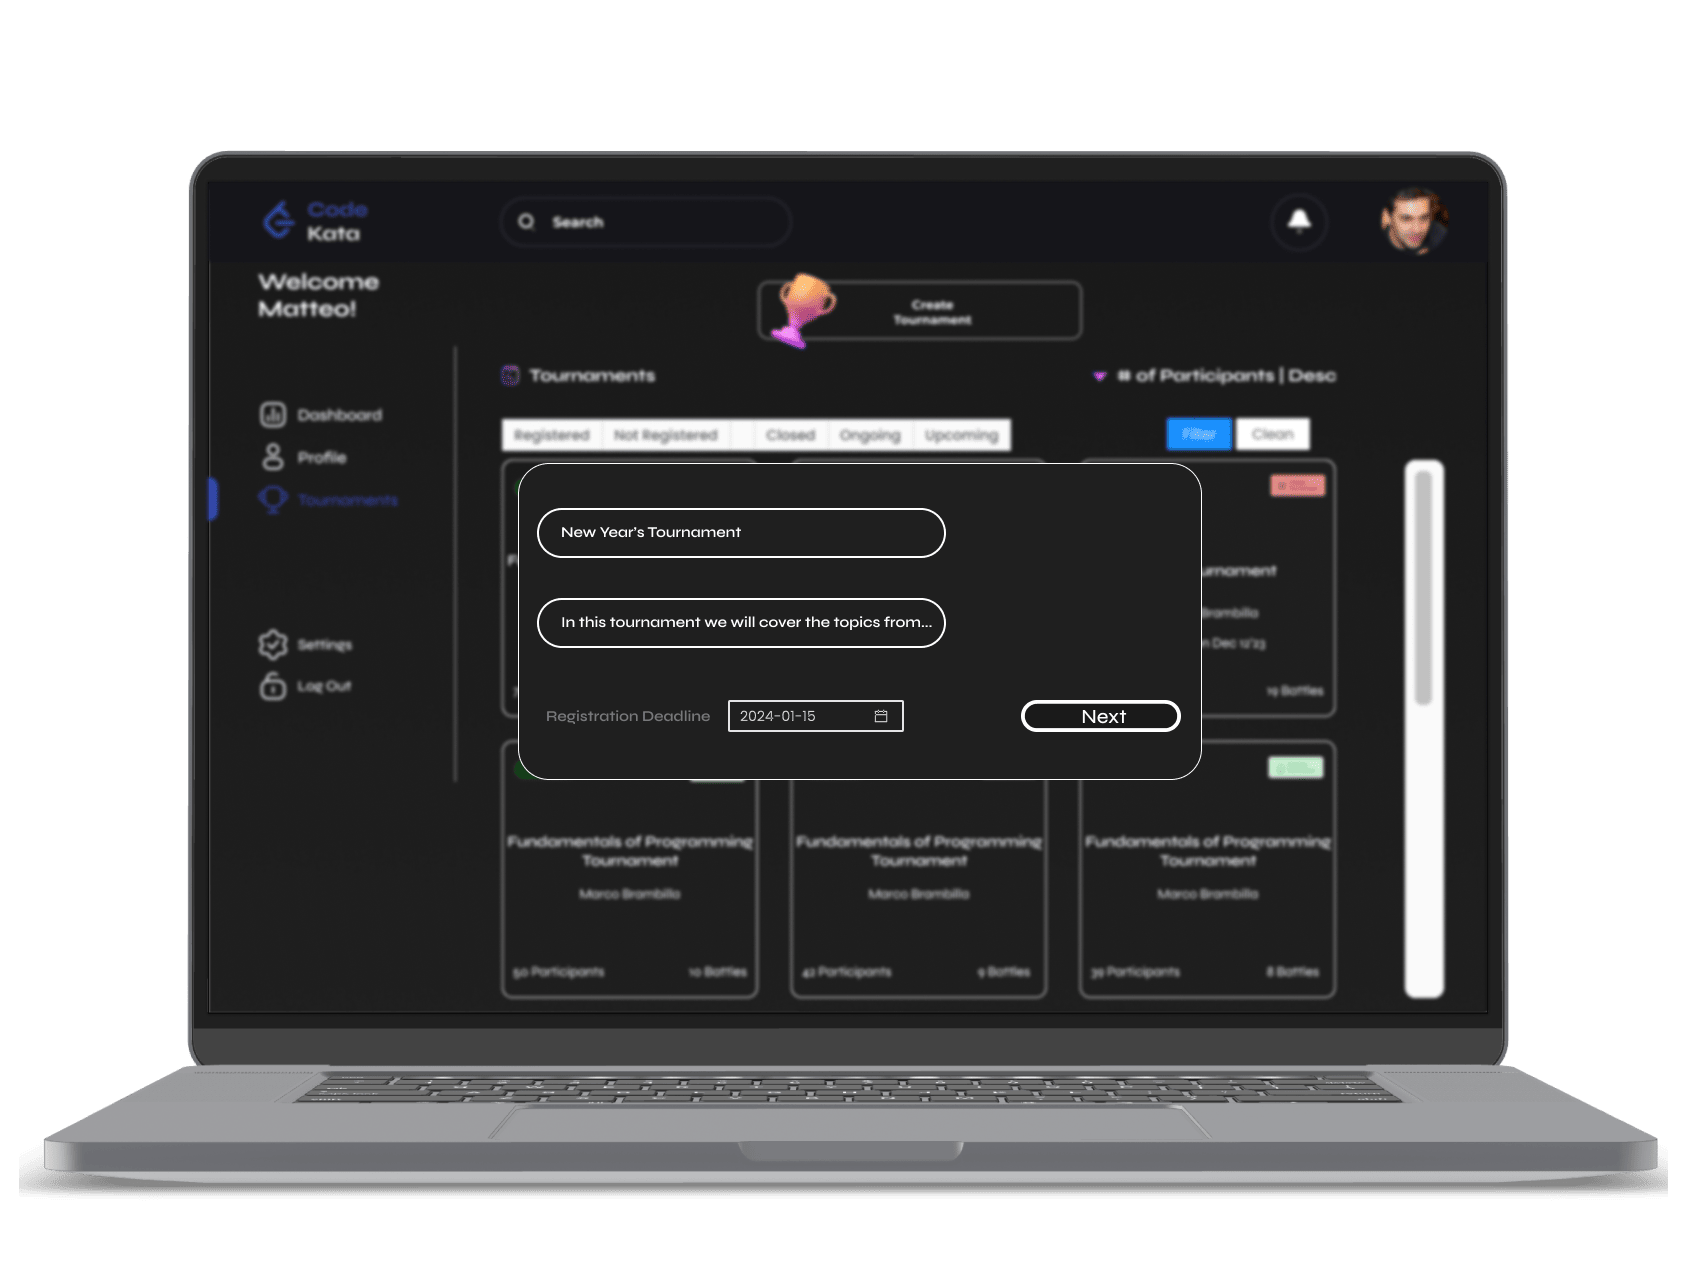
\includegraphics[scale=0.13]{Images/ui-ux/educator_create_tournament/educator_create_tournament_2.png}
% 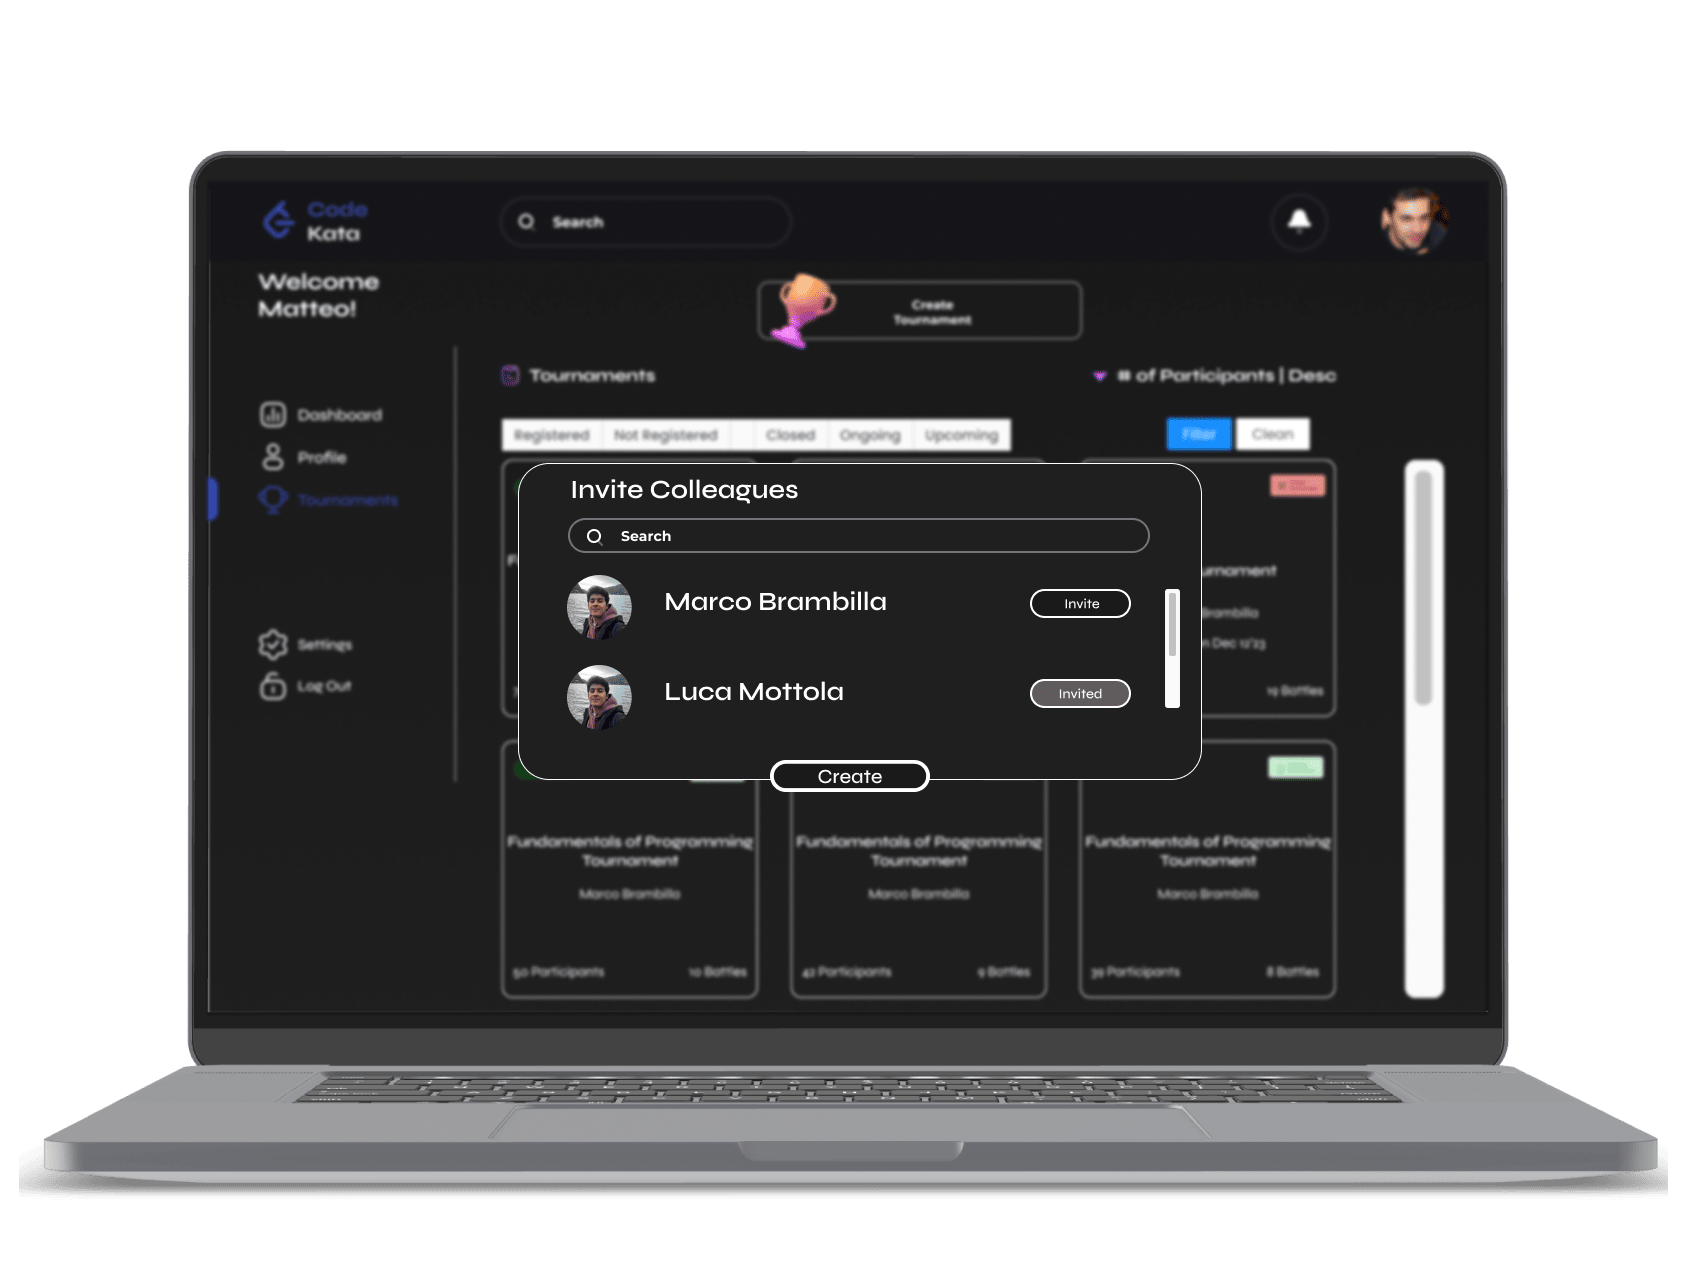
\includegraphics[scale=0.13]{Images/ui-ux/educator_create_tournament/educator_create_tournament_3.png}
% 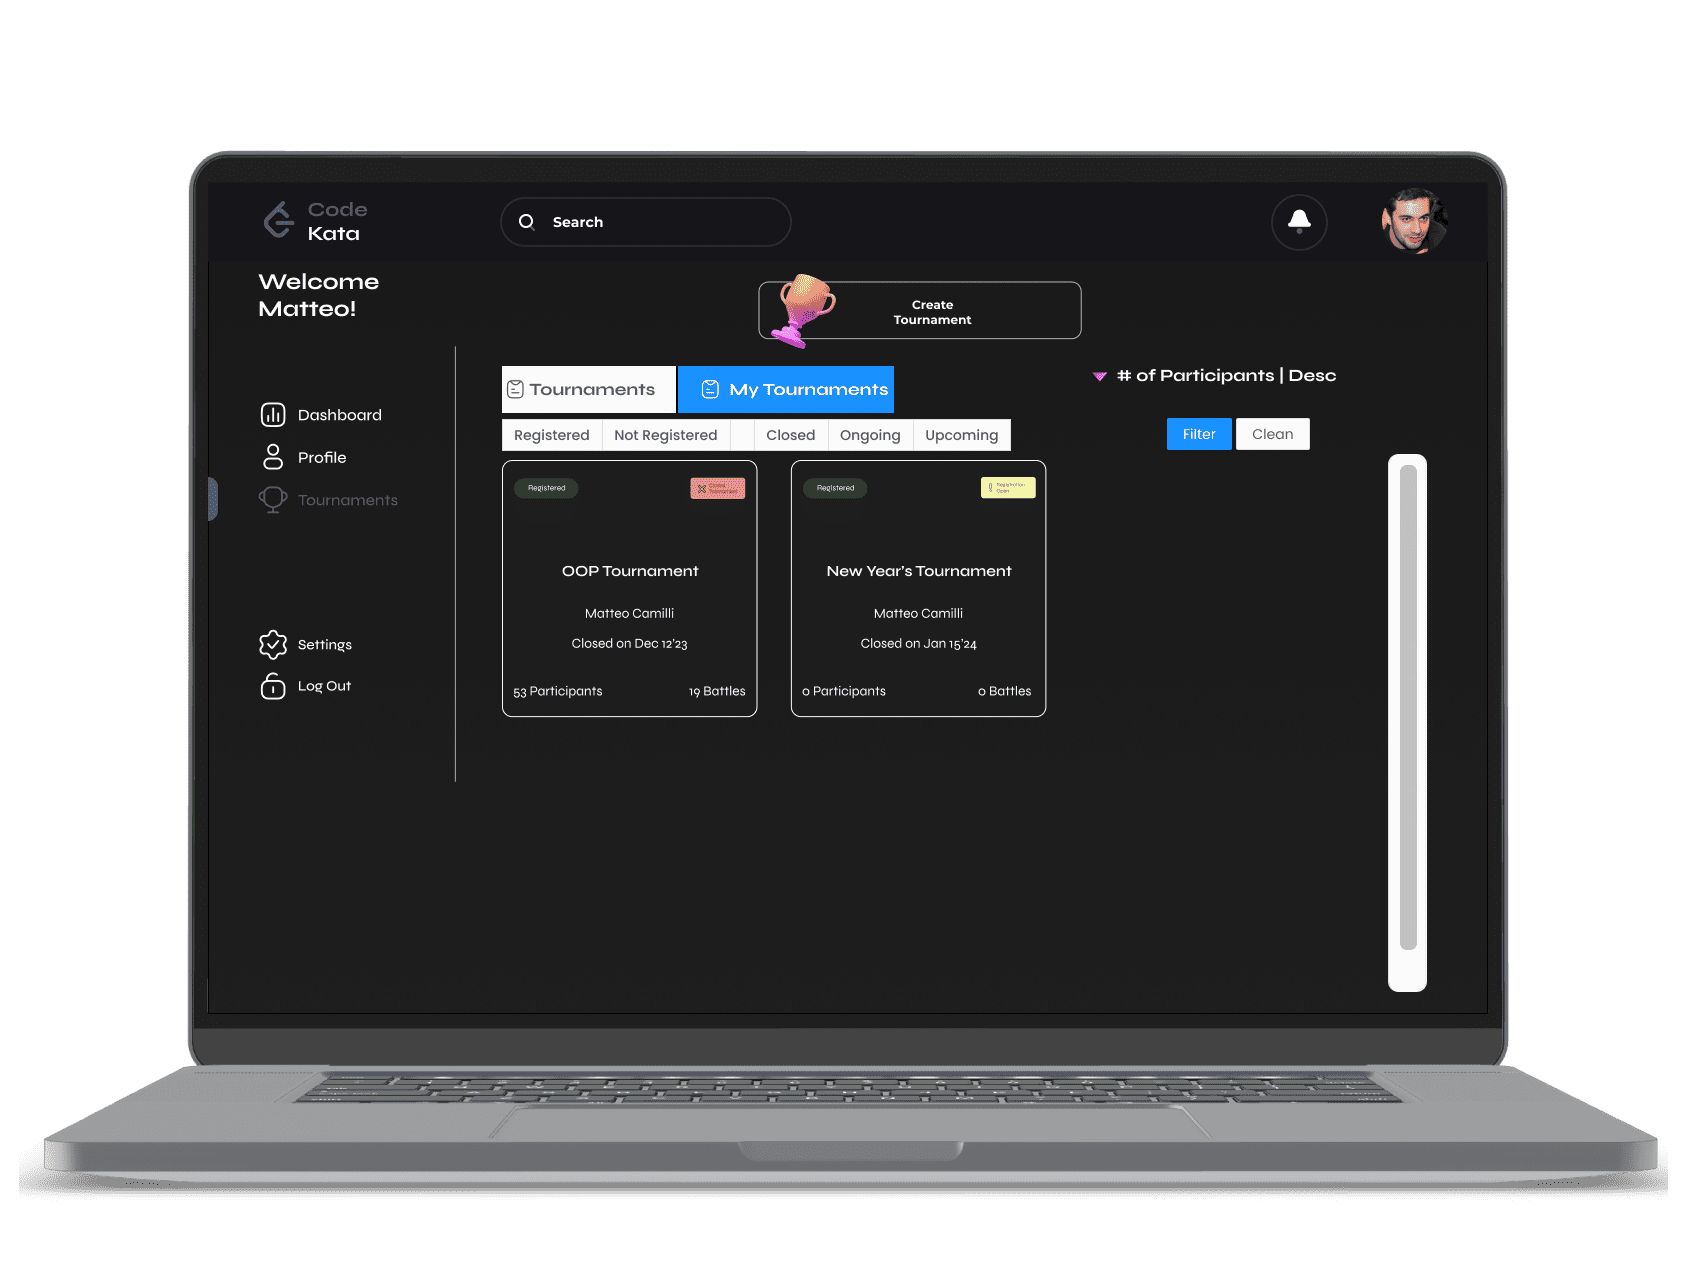
\includegraphics[scale=0.13]{Images/ui-ux/educator_create_tournament/educator_create_tournament_4.png}
%         (a) Educator Creates Tournaments
% \end{center}
% \begin{center}
% 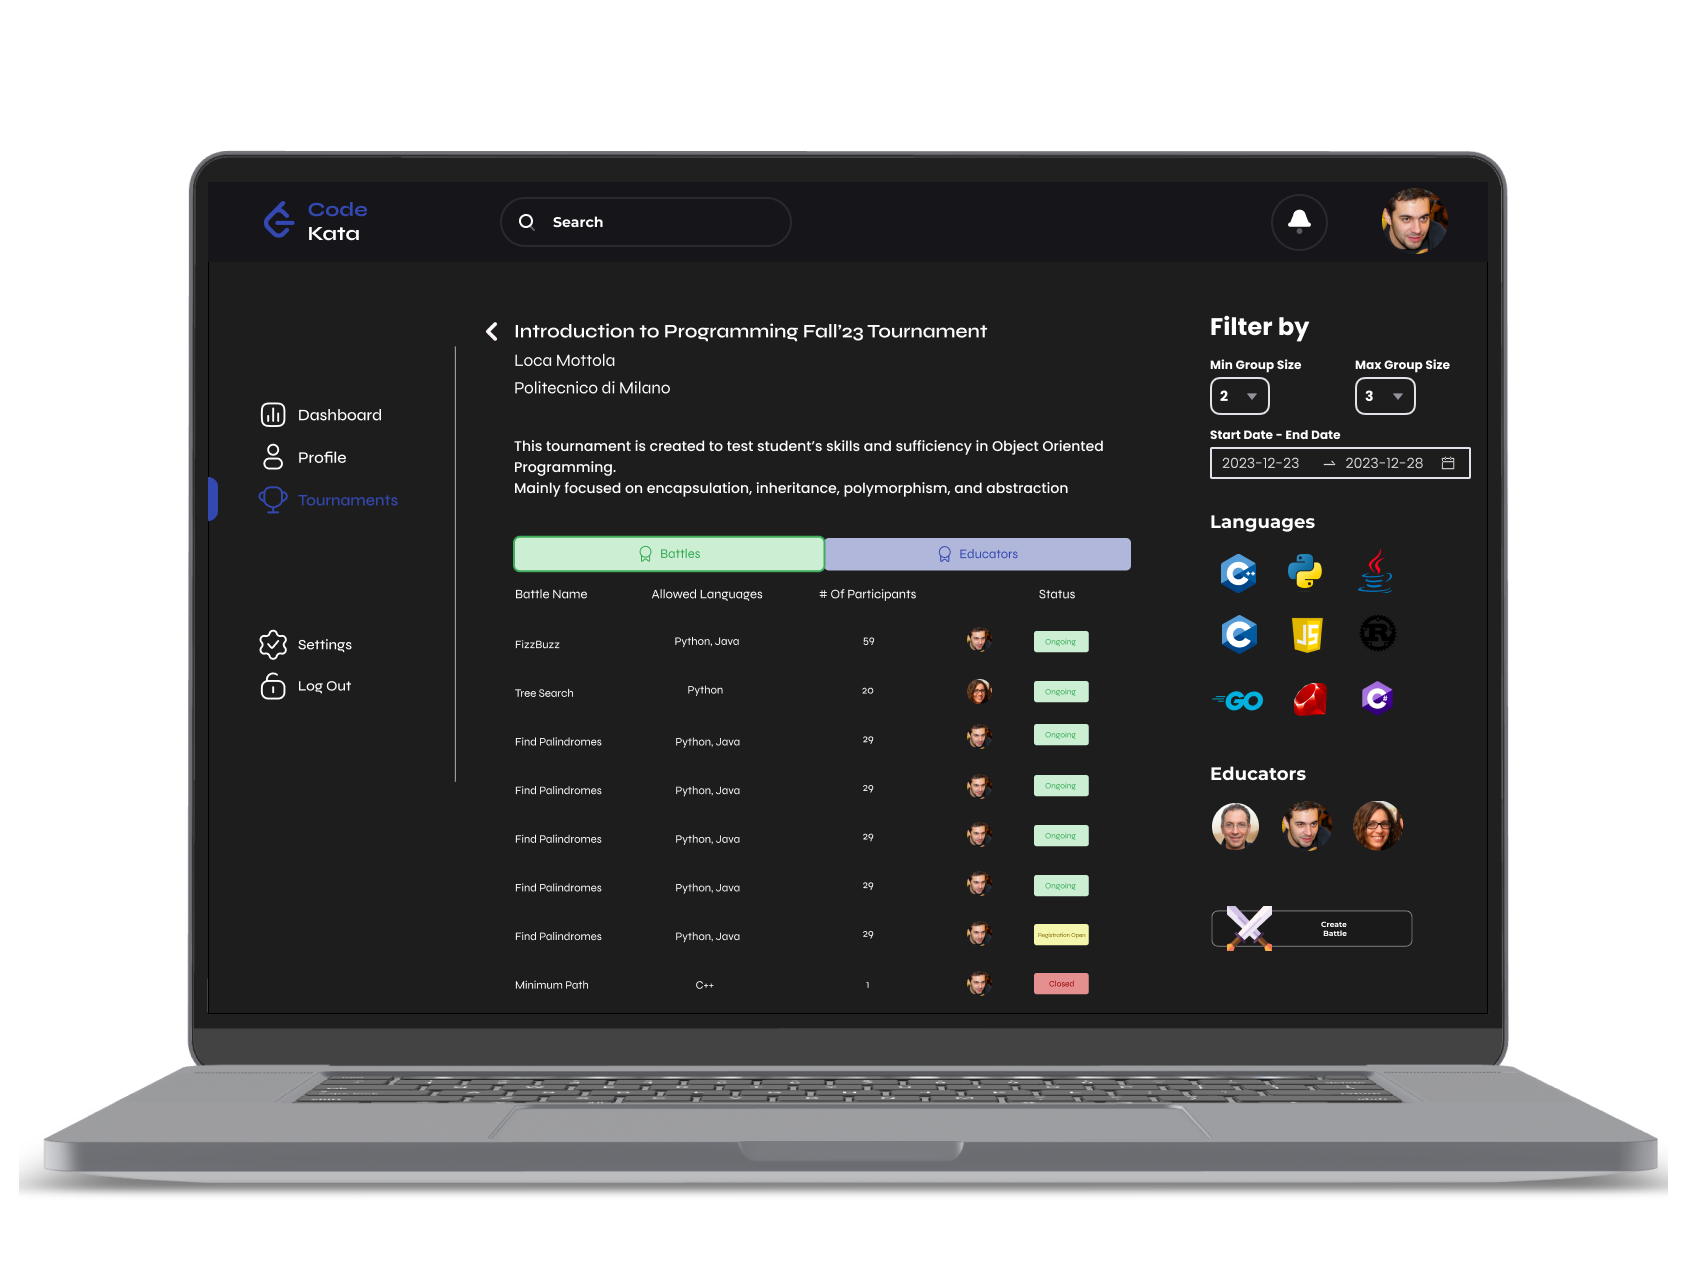
\includegraphics[scale=0.13]{Images/ui-ux/educator_creates_battle/educator_creates_battle_1.png}
% 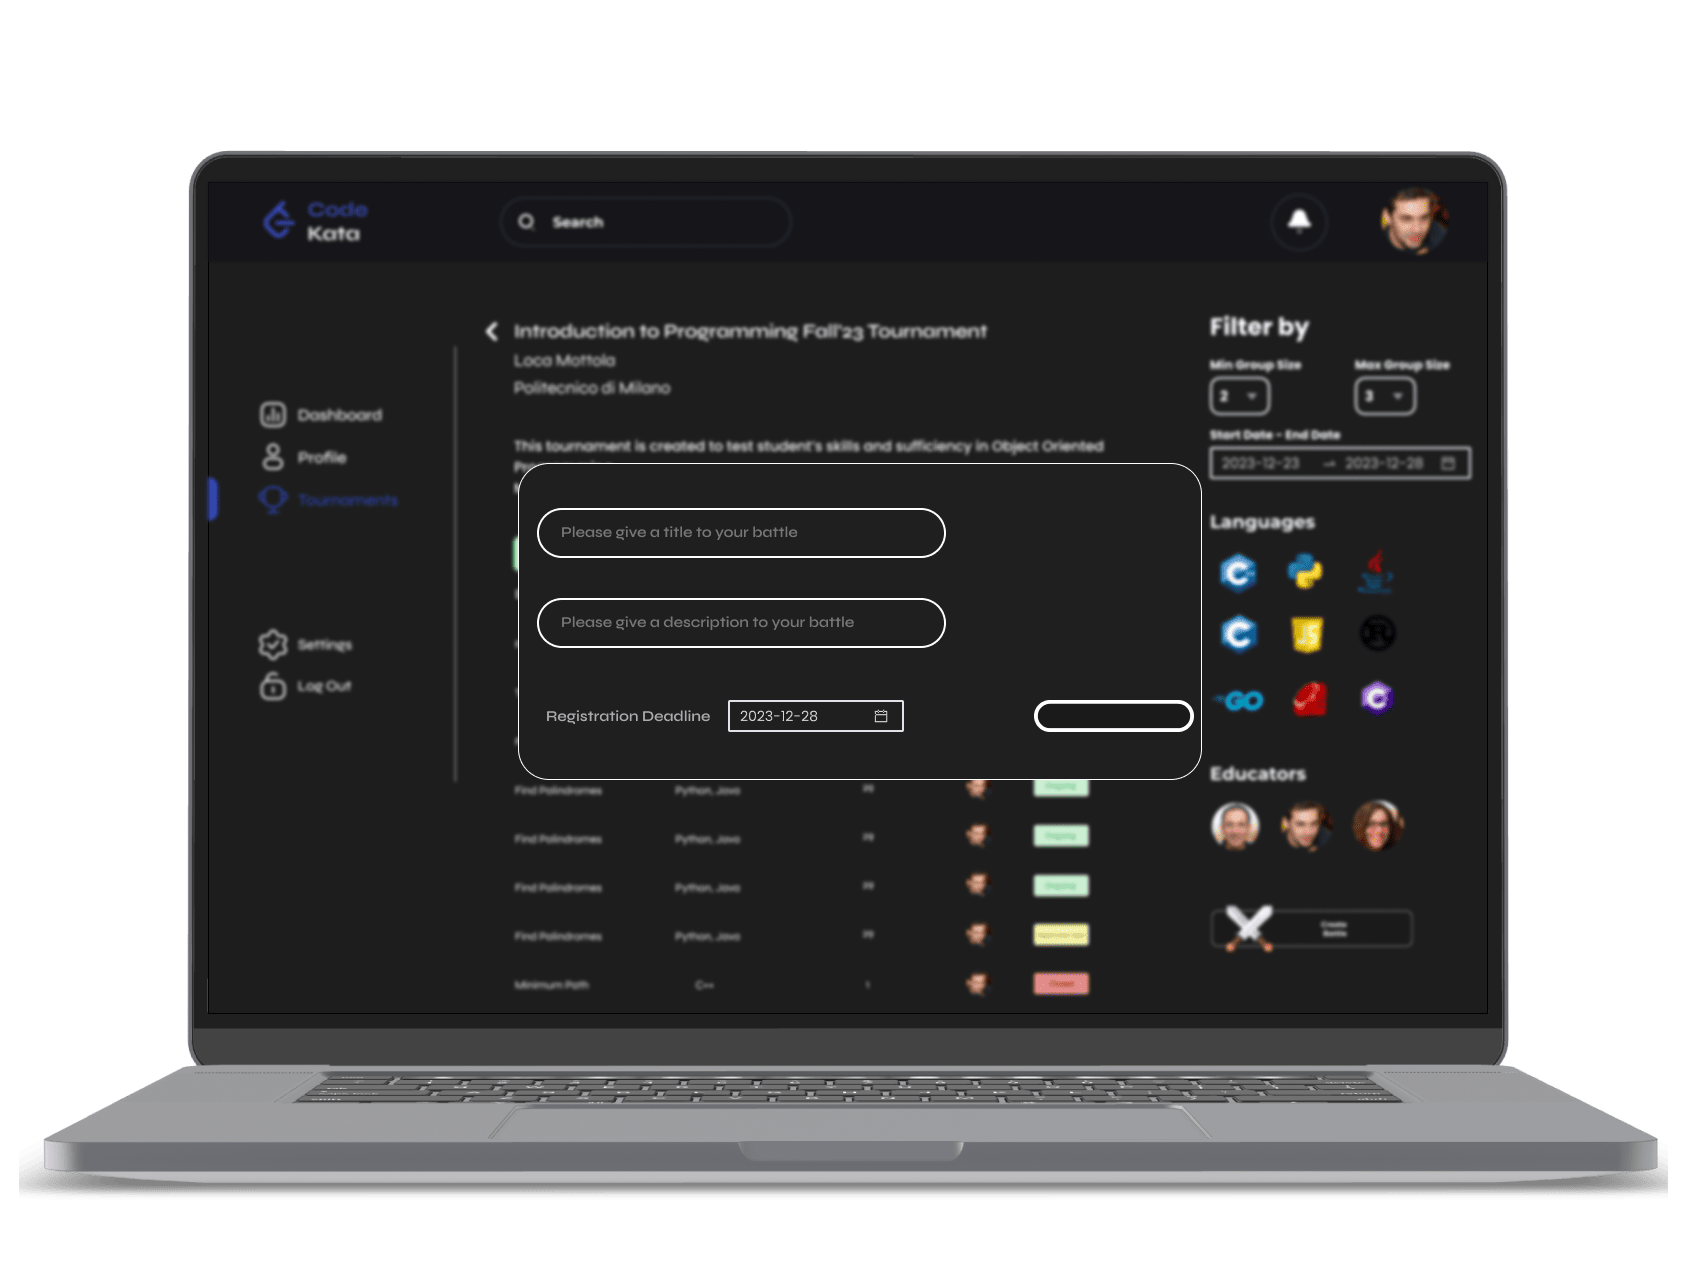
\includegraphics[scale=0.13]{Images/ui-ux/educator_creates_battle/educator_creates_battle_2.png}
% 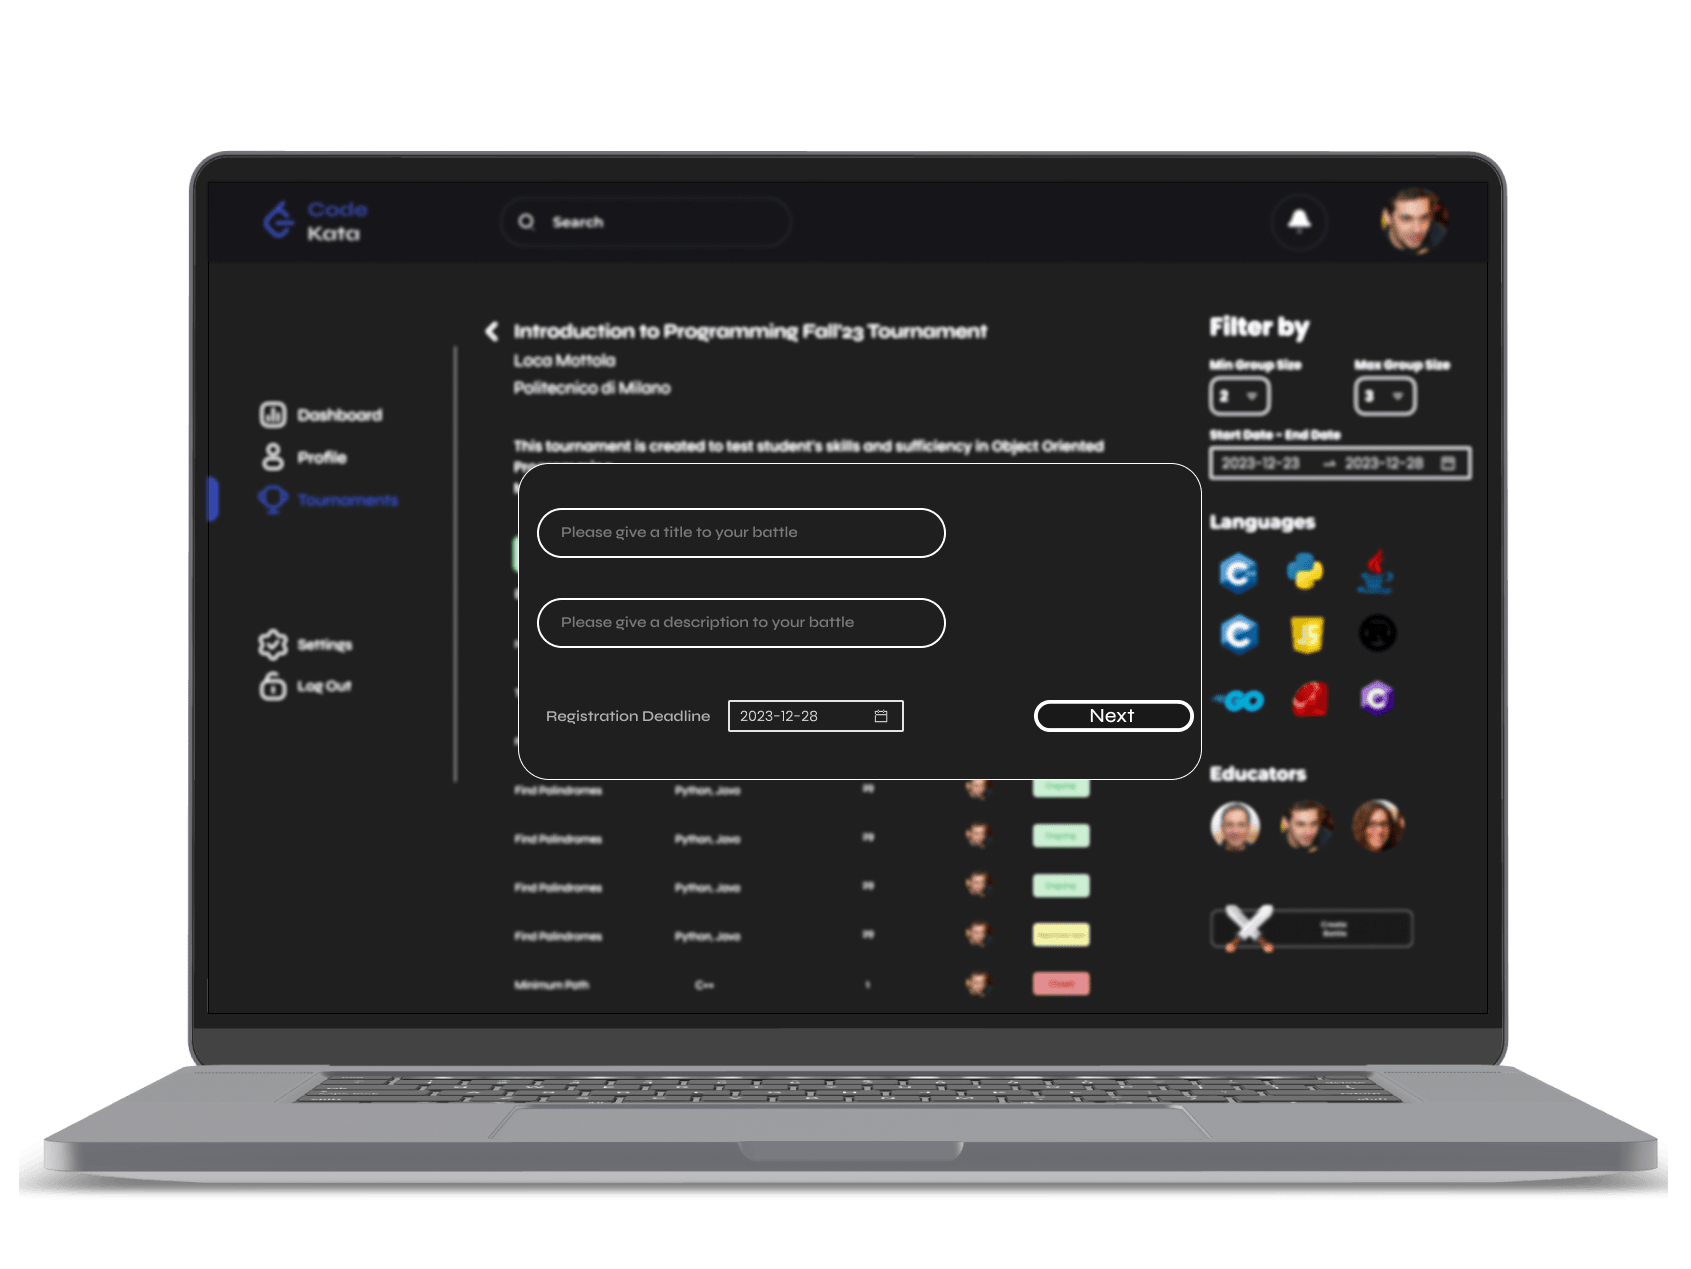
\includegraphics[scale=0.13]{Images/ui-ux/educator_creates_battle/educator_creates_battle_3.png}
% 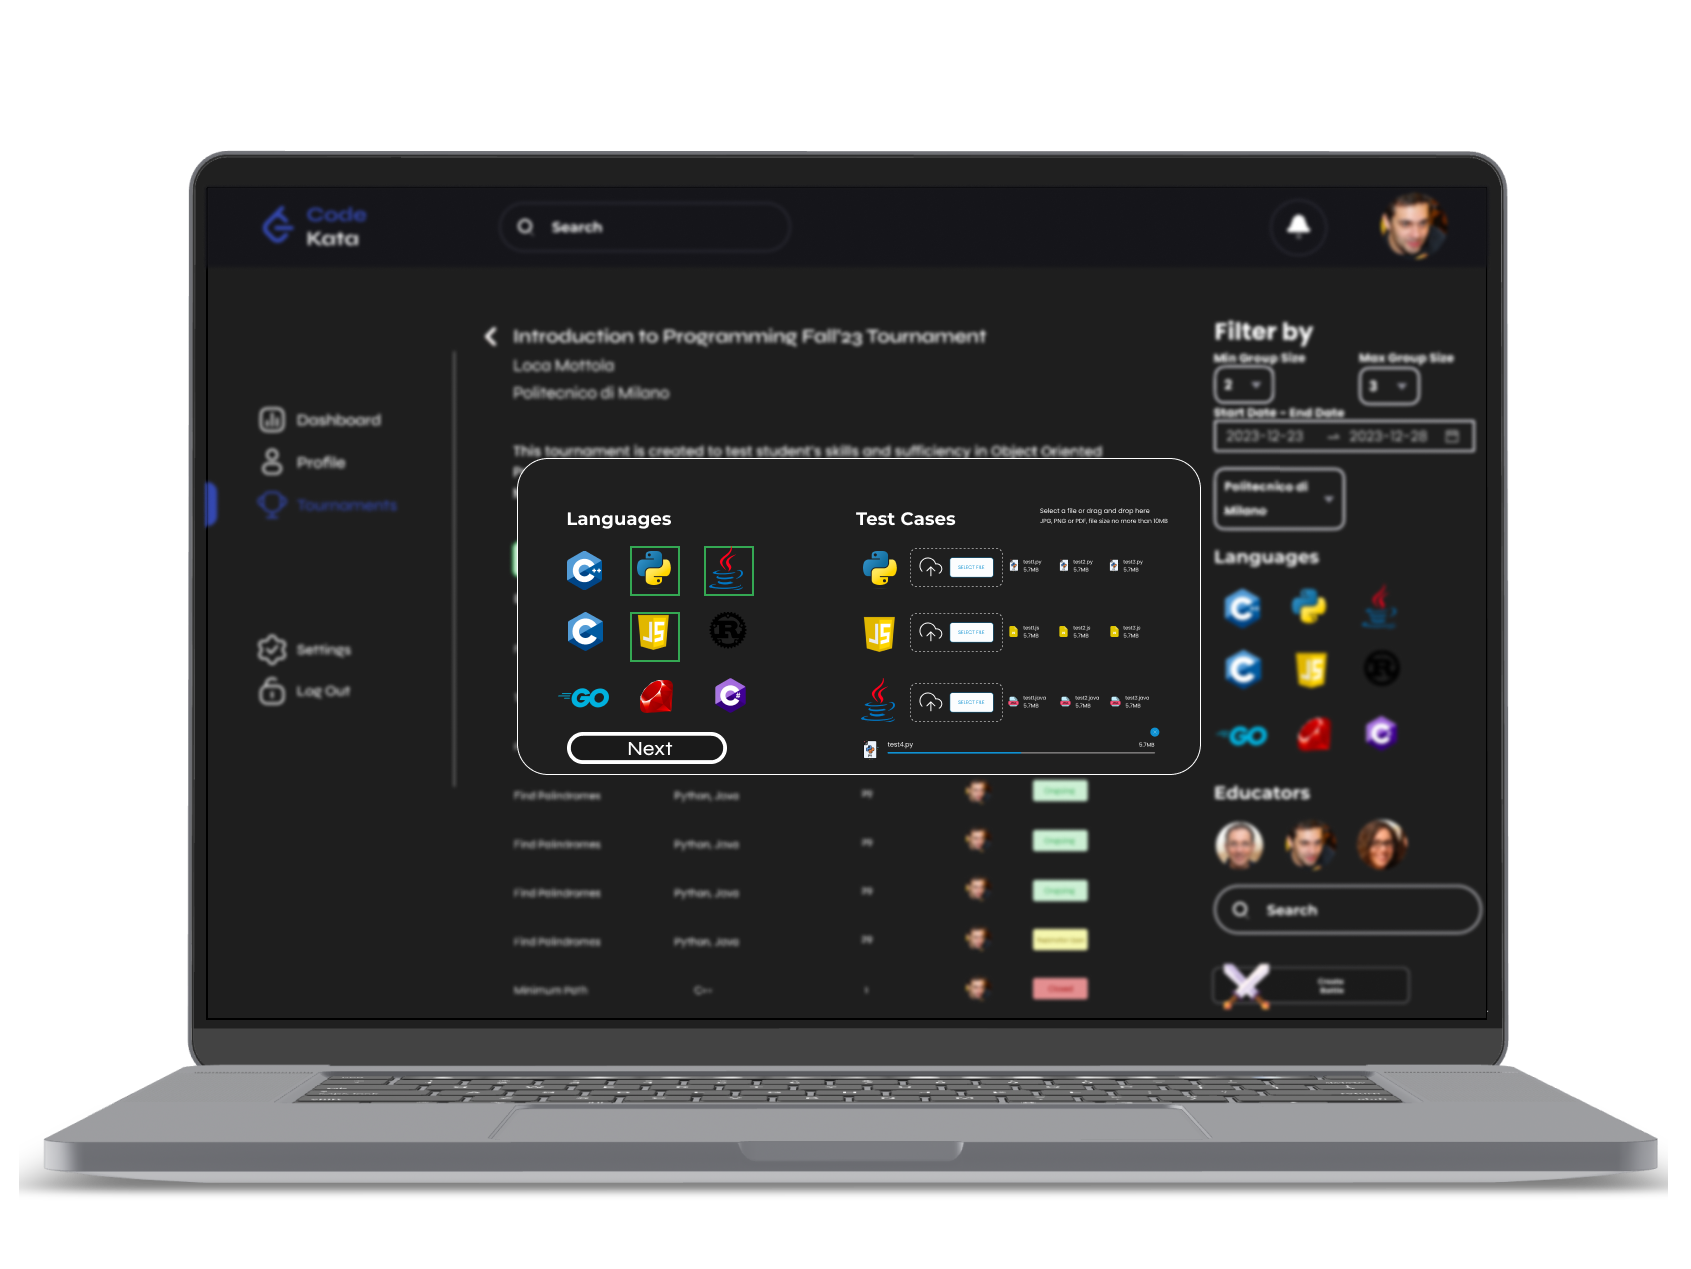
\includegraphics[scale=0.13]{Images/ui-ux/educator_creates_battle/educator_creates_battle_4.png}
% 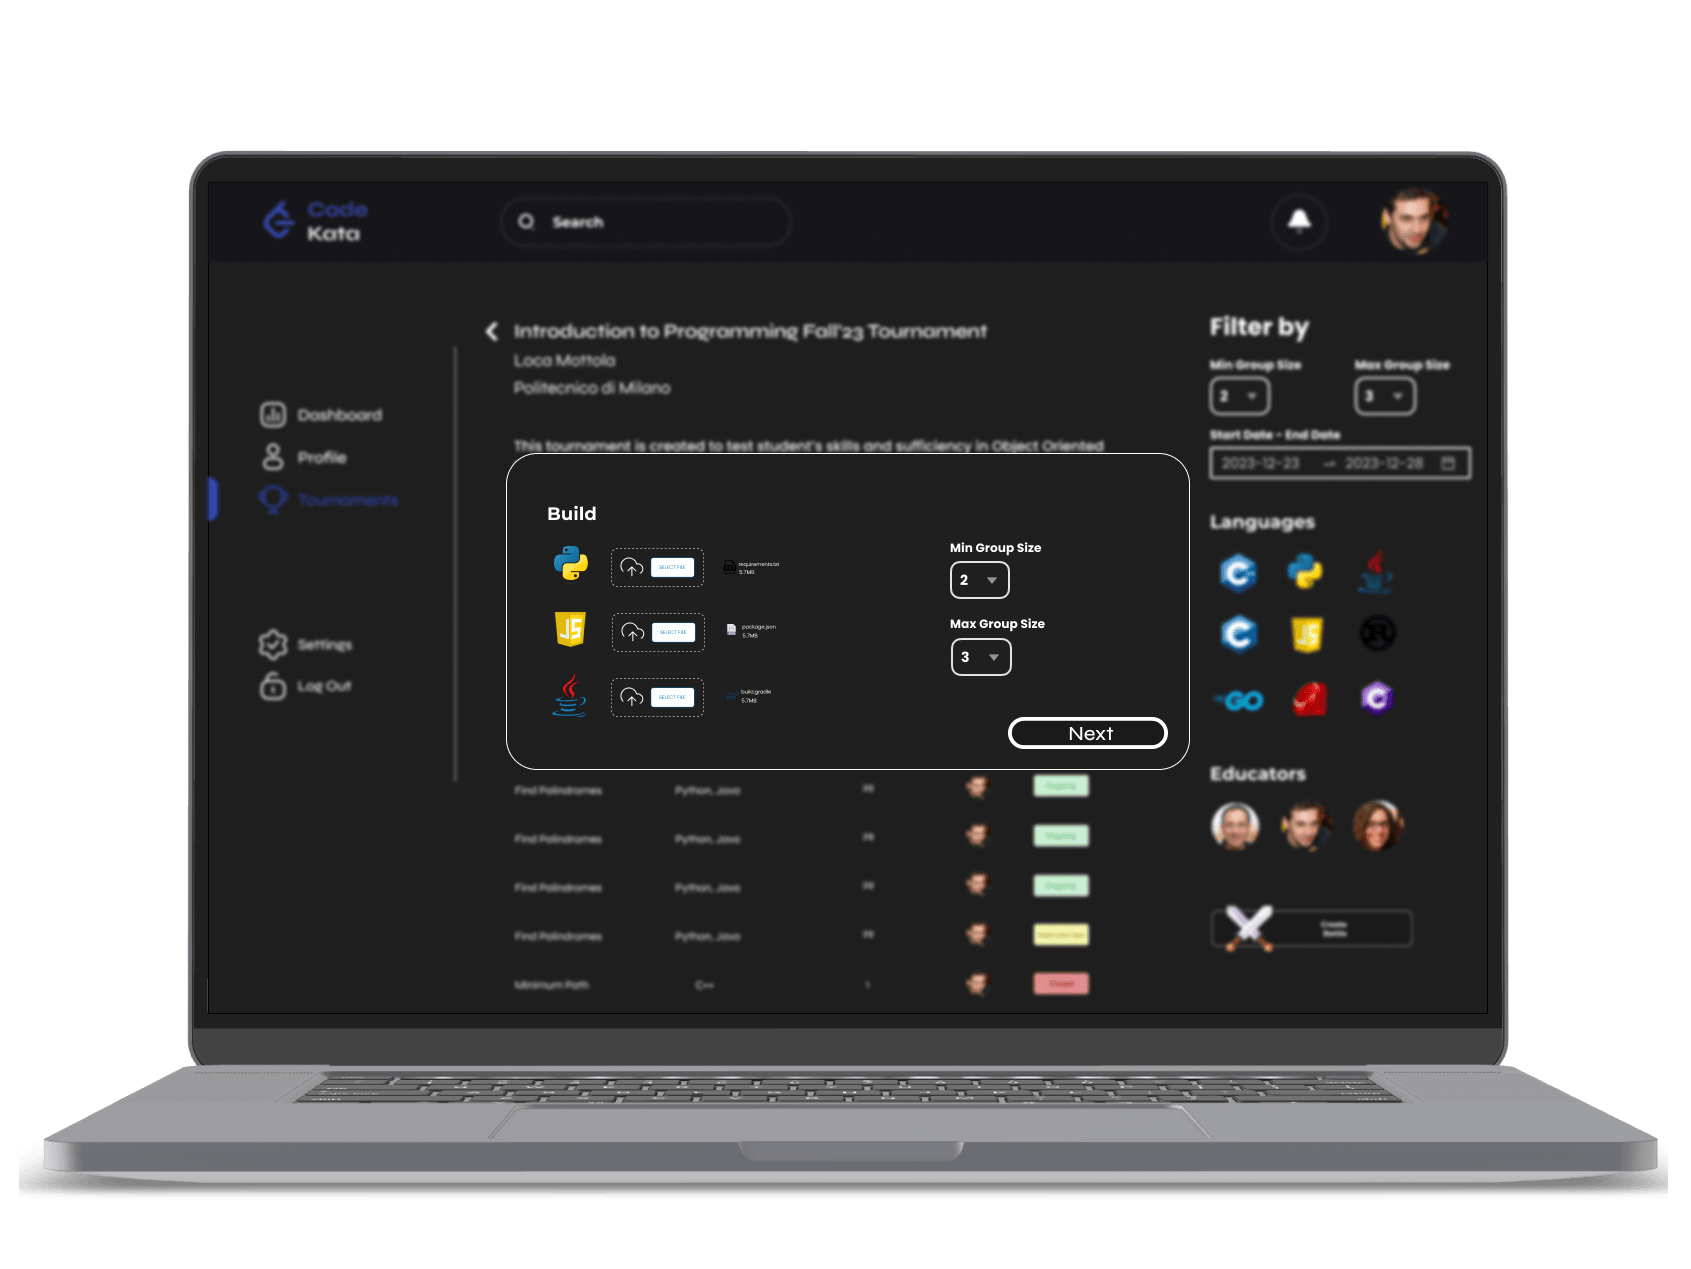
\includegraphics[scale=0.13]{Images/ui-ux/educator_creates_battle/educator_creates_battle_5.png}
% 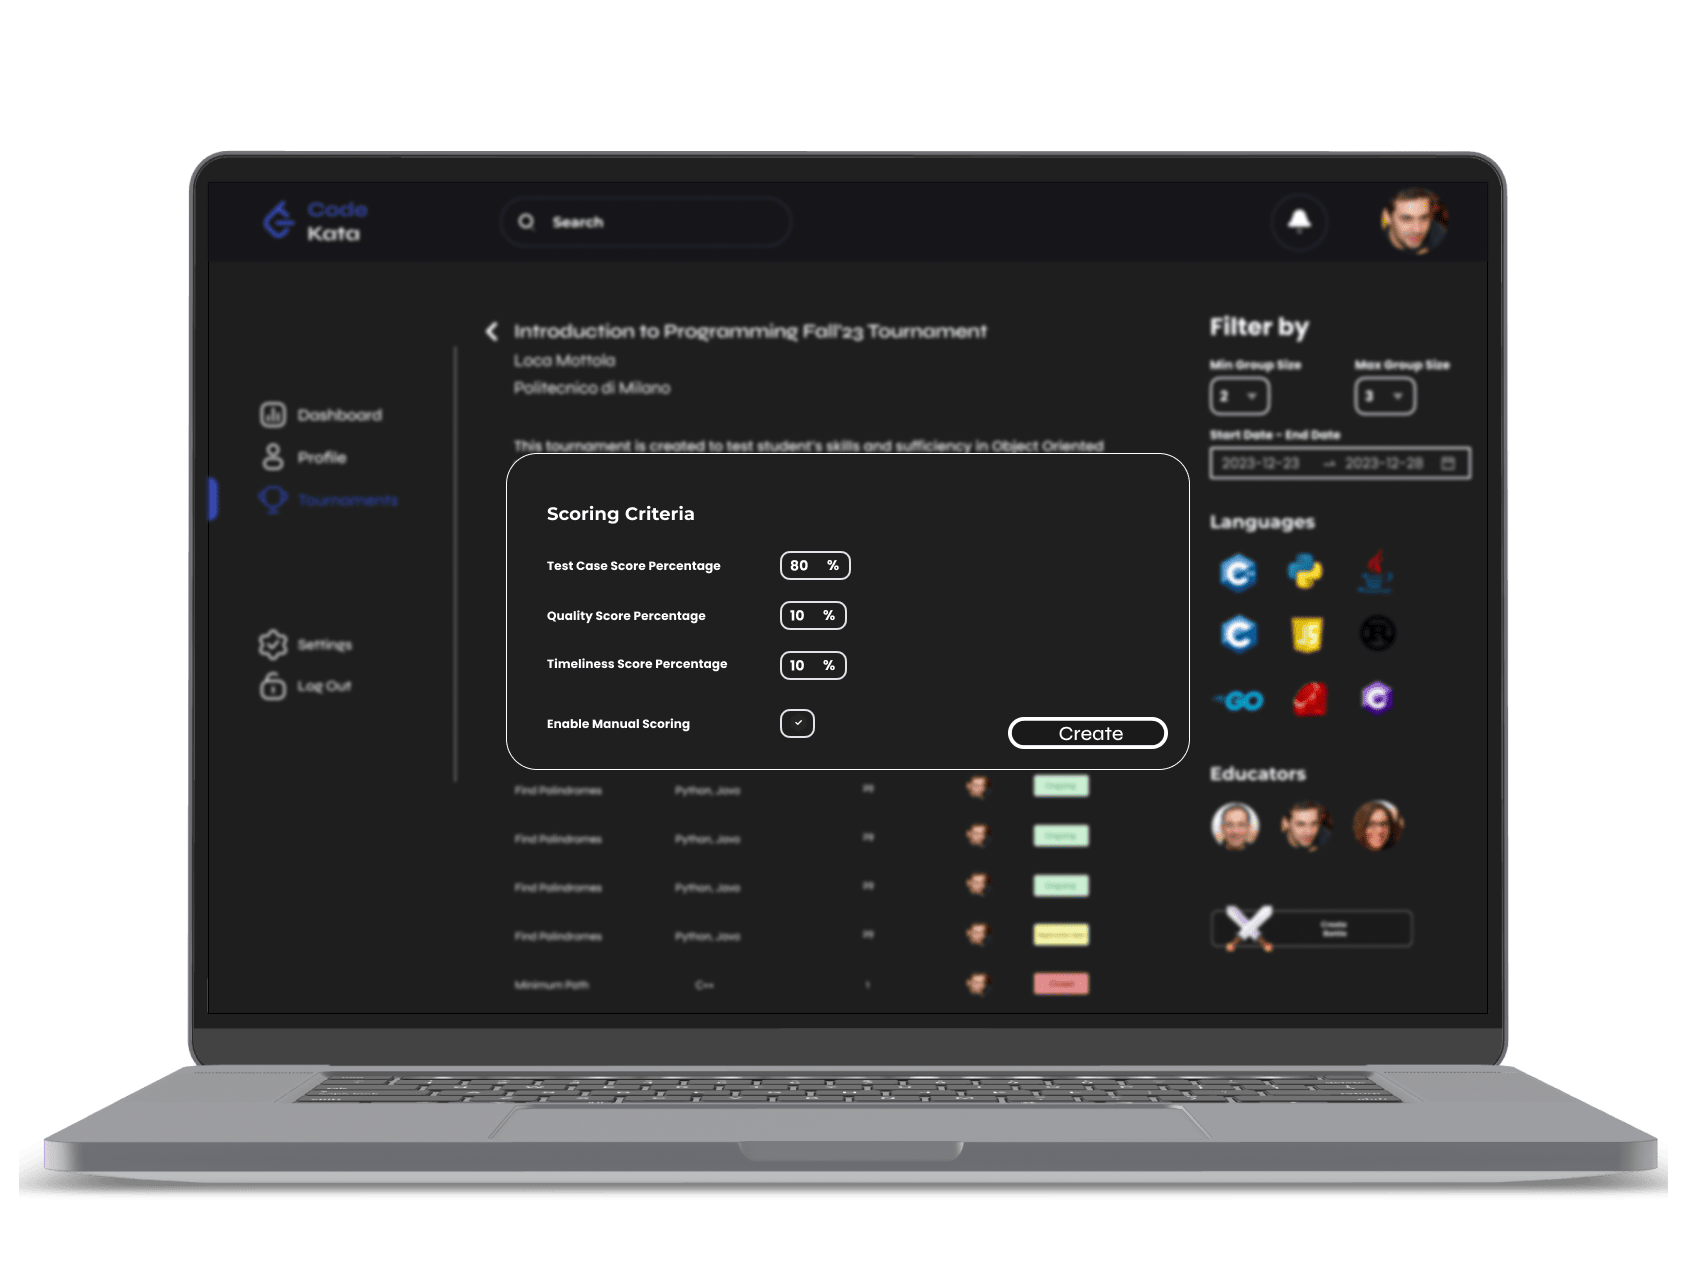
\includegraphics[scale=0.13]{Images/ui-ux/educator_creates_battle/educator_creates_battle_6.png}
%         (a) Educator Creates Battle
% \end{center}
% \begin{center}
% 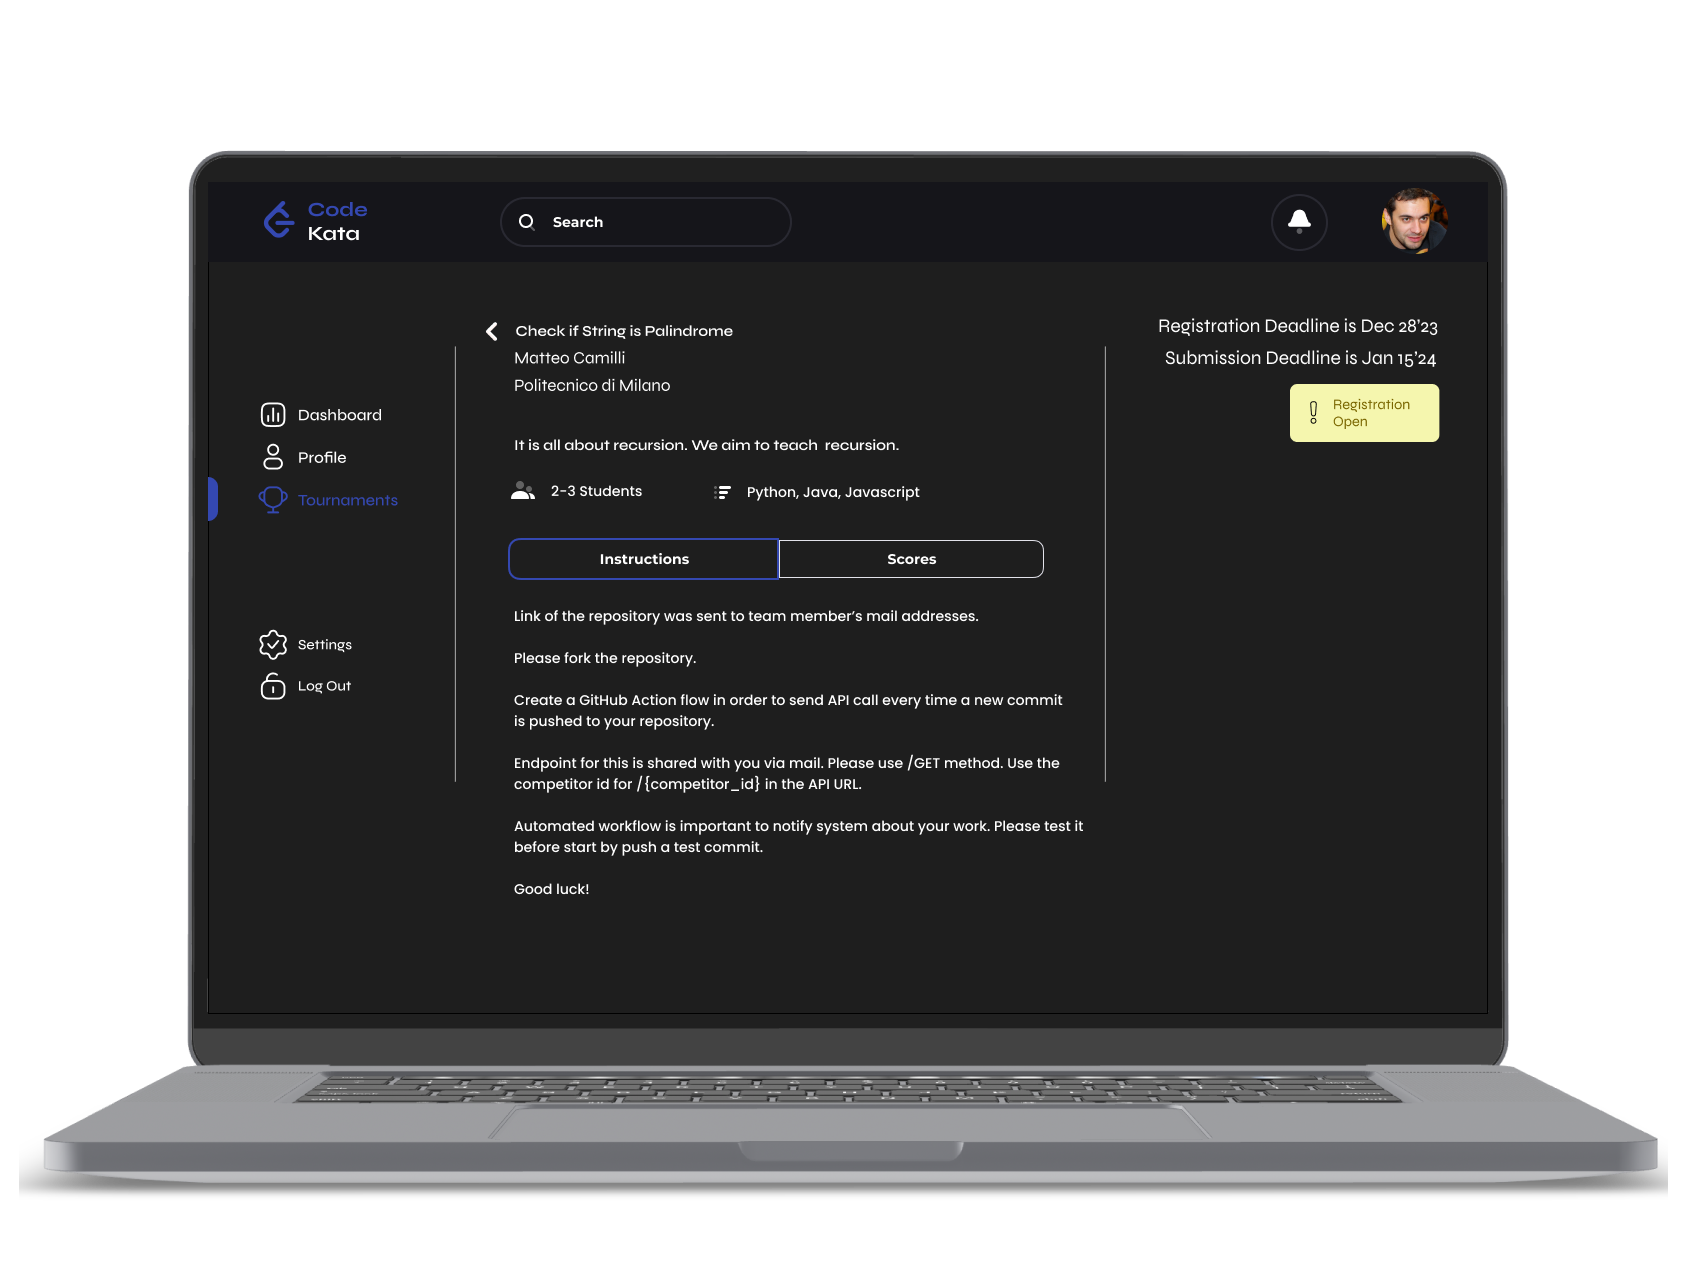
\includegraphics[scale=0.13]{Images/ui-ux/educator_battle/educator_battle_1.png}
% 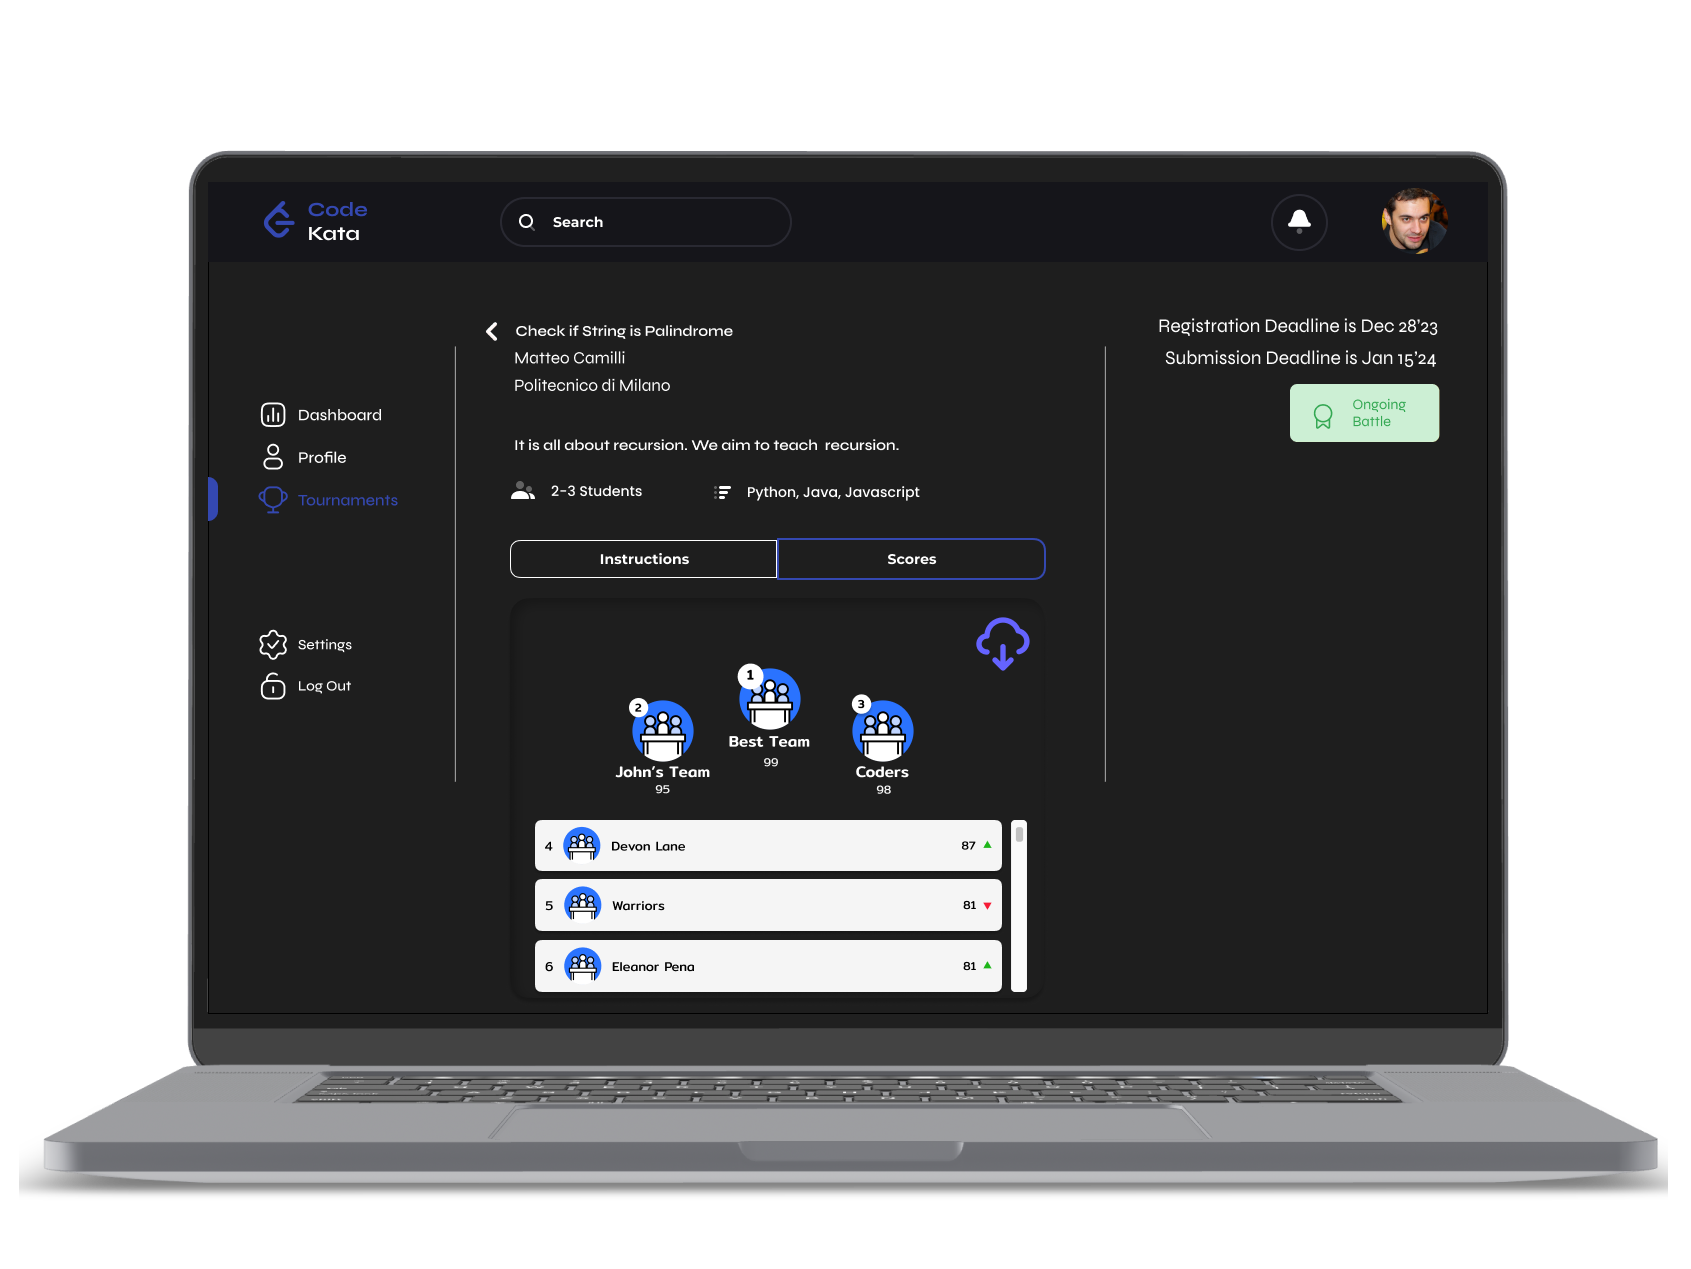
\includegraphics[scale=0.13]{Images/ui-ux/educator_battle/educator_battle_2.png}
% 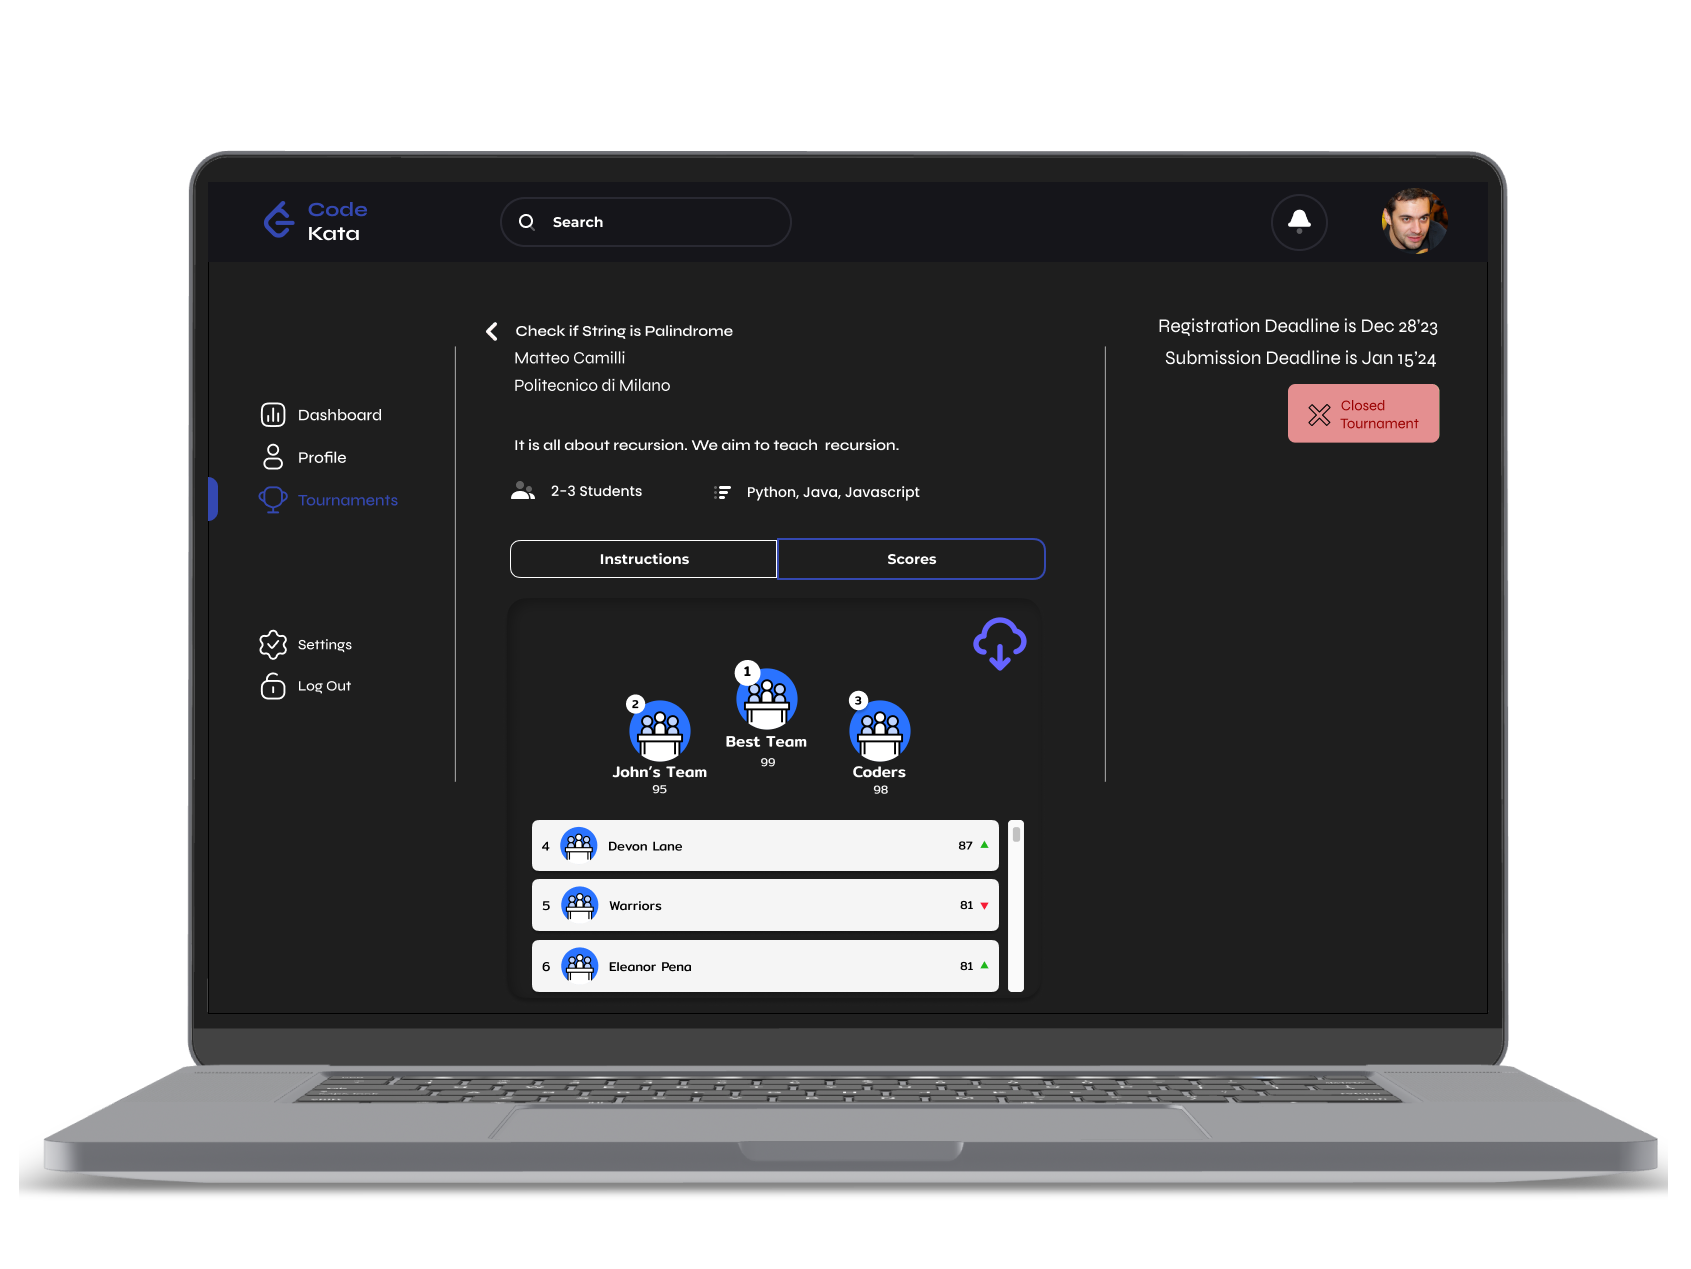
\includegraphics[scale=0.13]{Images/ui-ux/educator_battle/educator_battle_3.png}
%  \\(a) Educator and Battle
% \end{center}
% \begin{center}
% 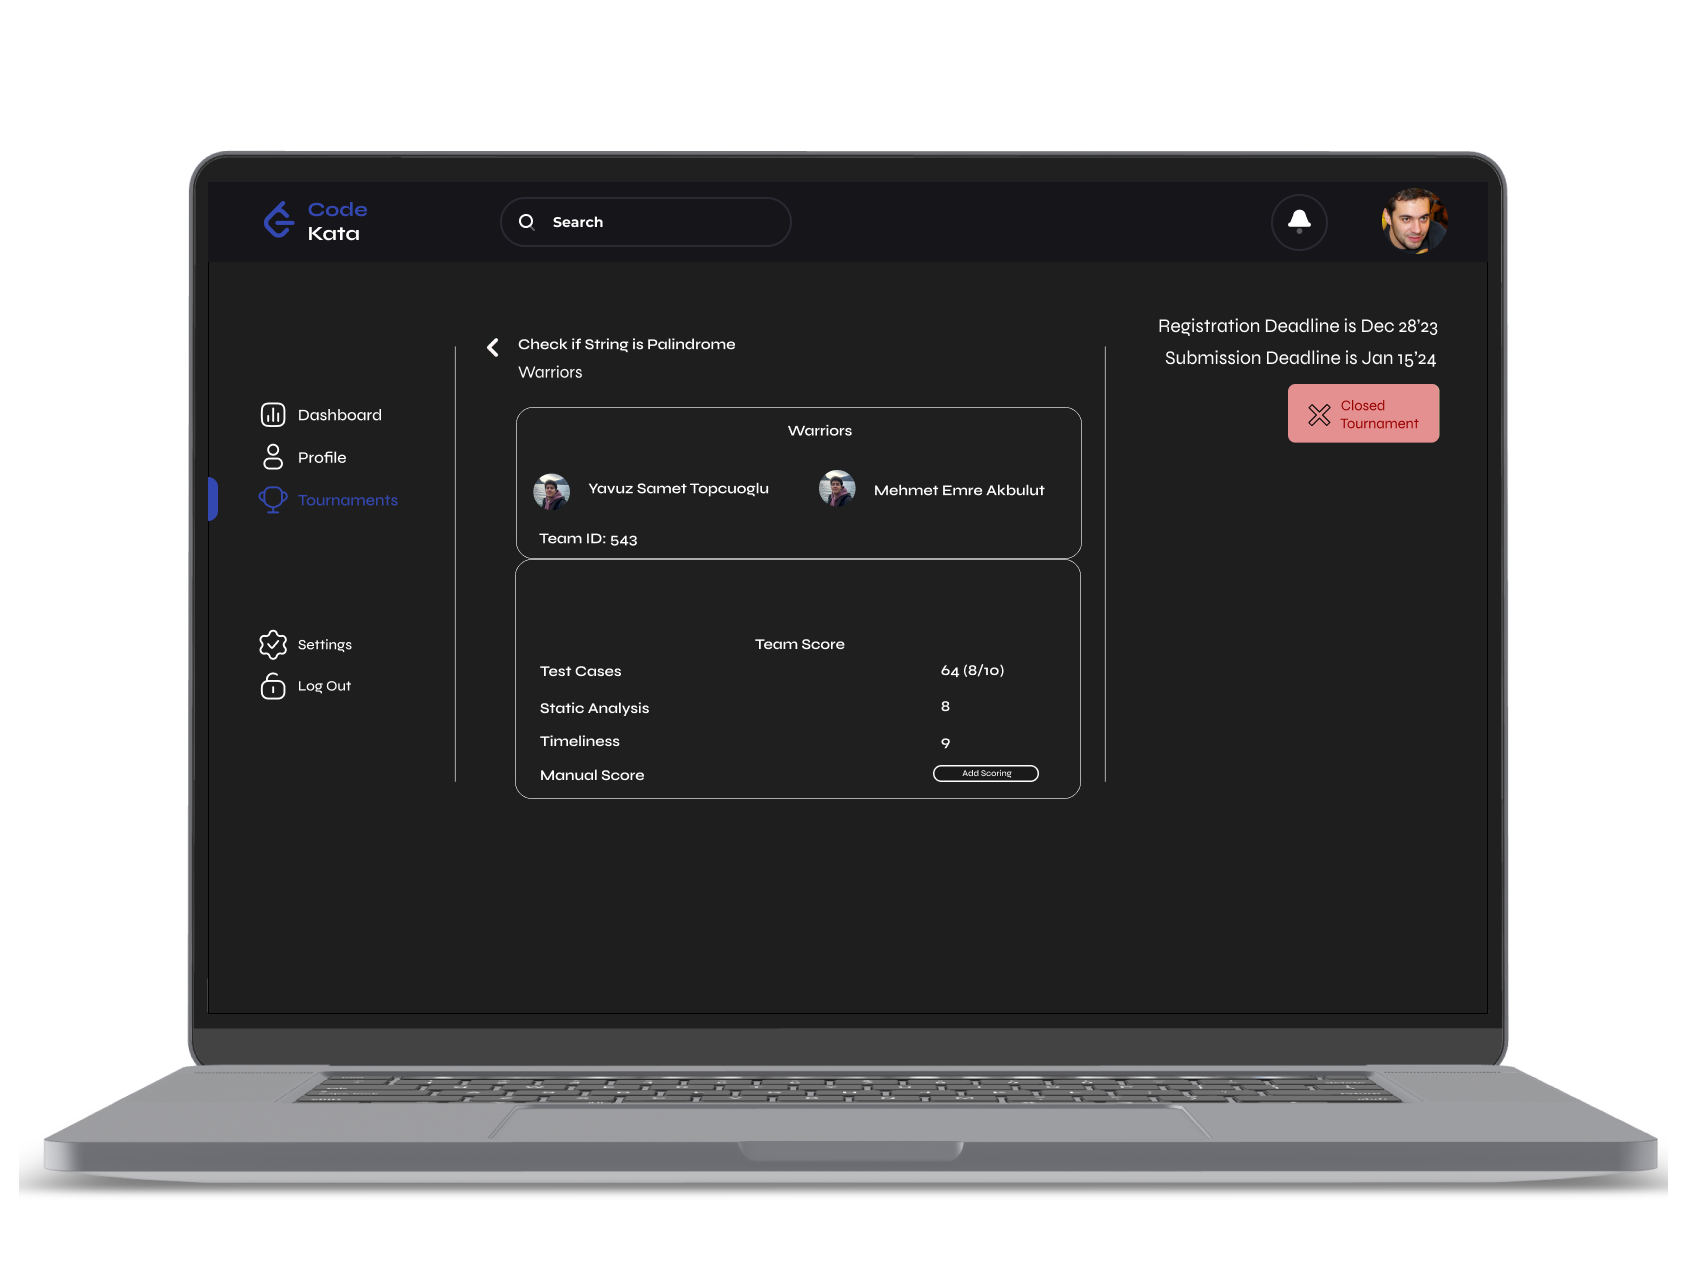
\includegraphics[scale=0.13]{Images/ui-ux/educator_team/educator_team_1.png}
% 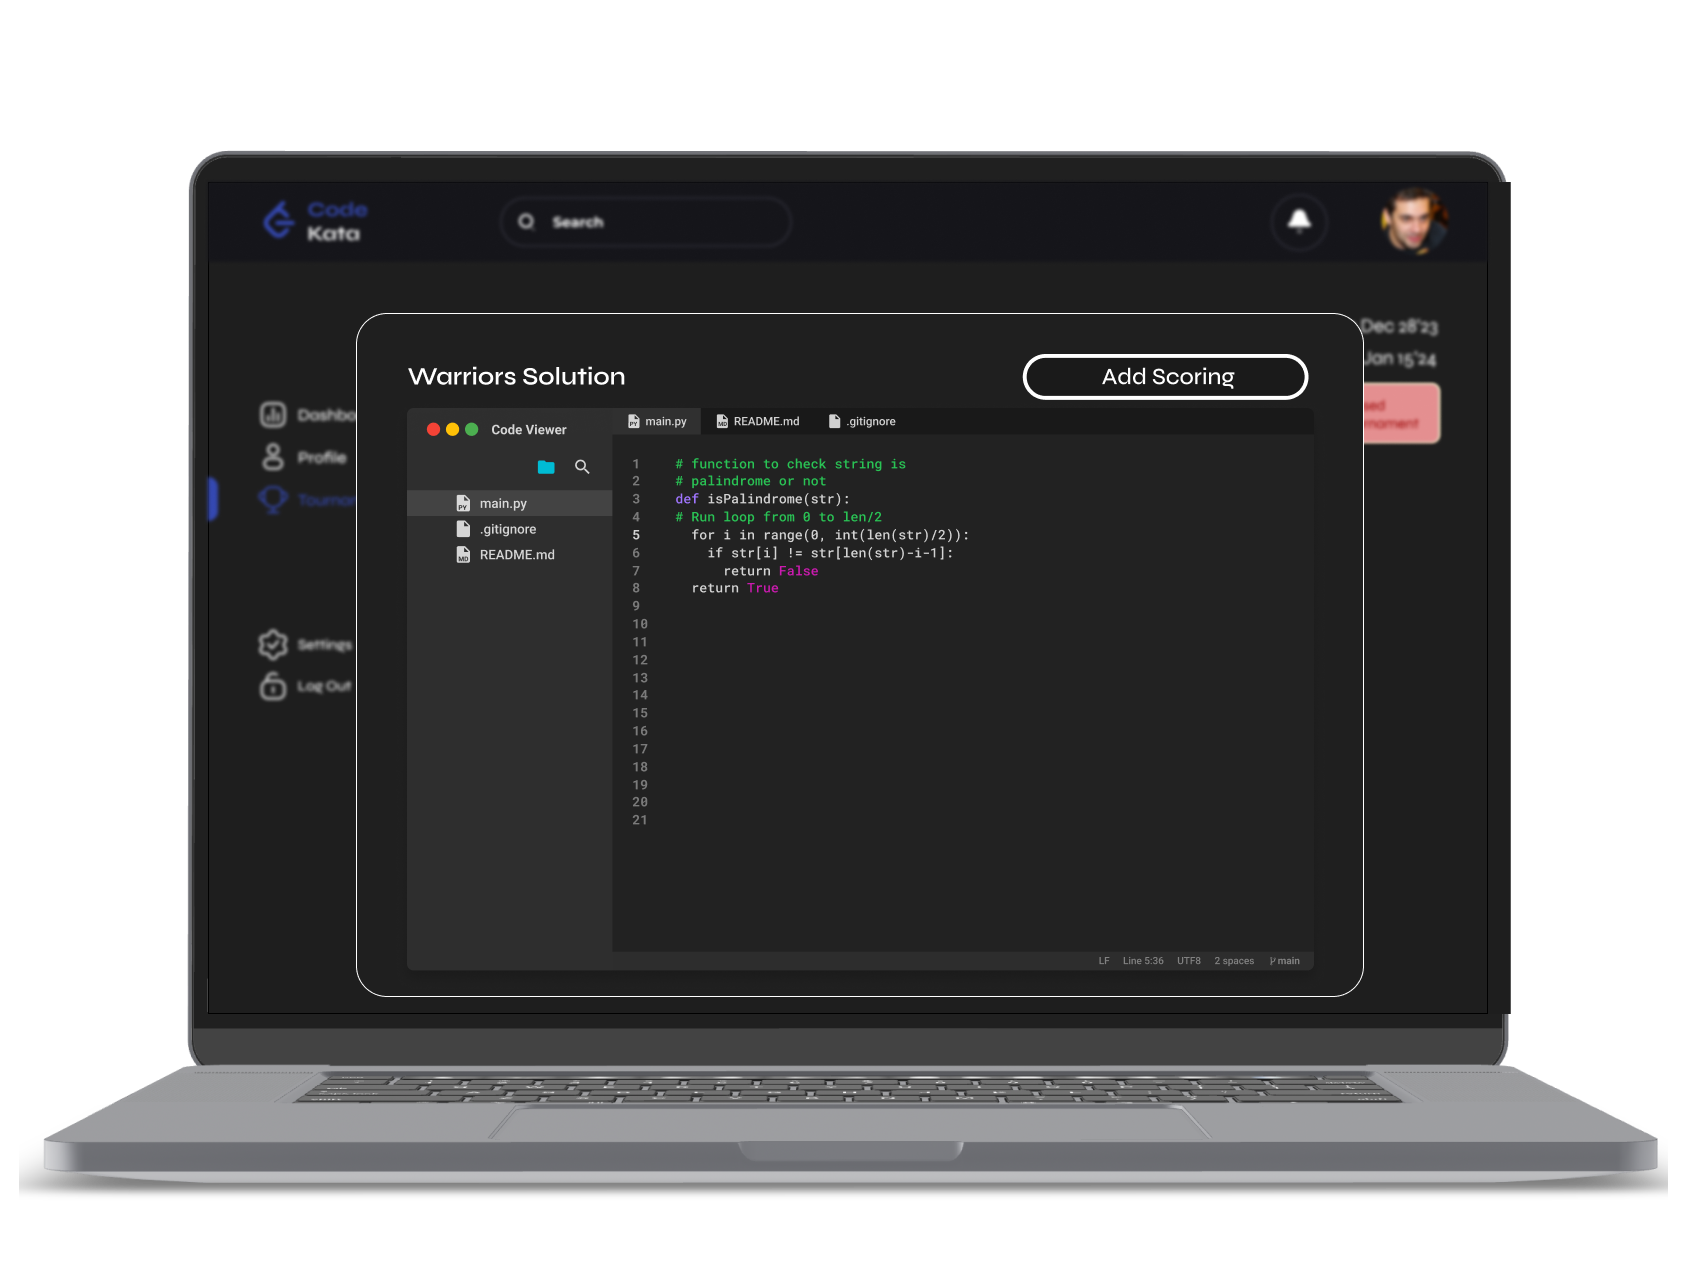
\includegraphics[scale=0.13]{Images/ui-ux/educator_team/educator_team_2.png}
% 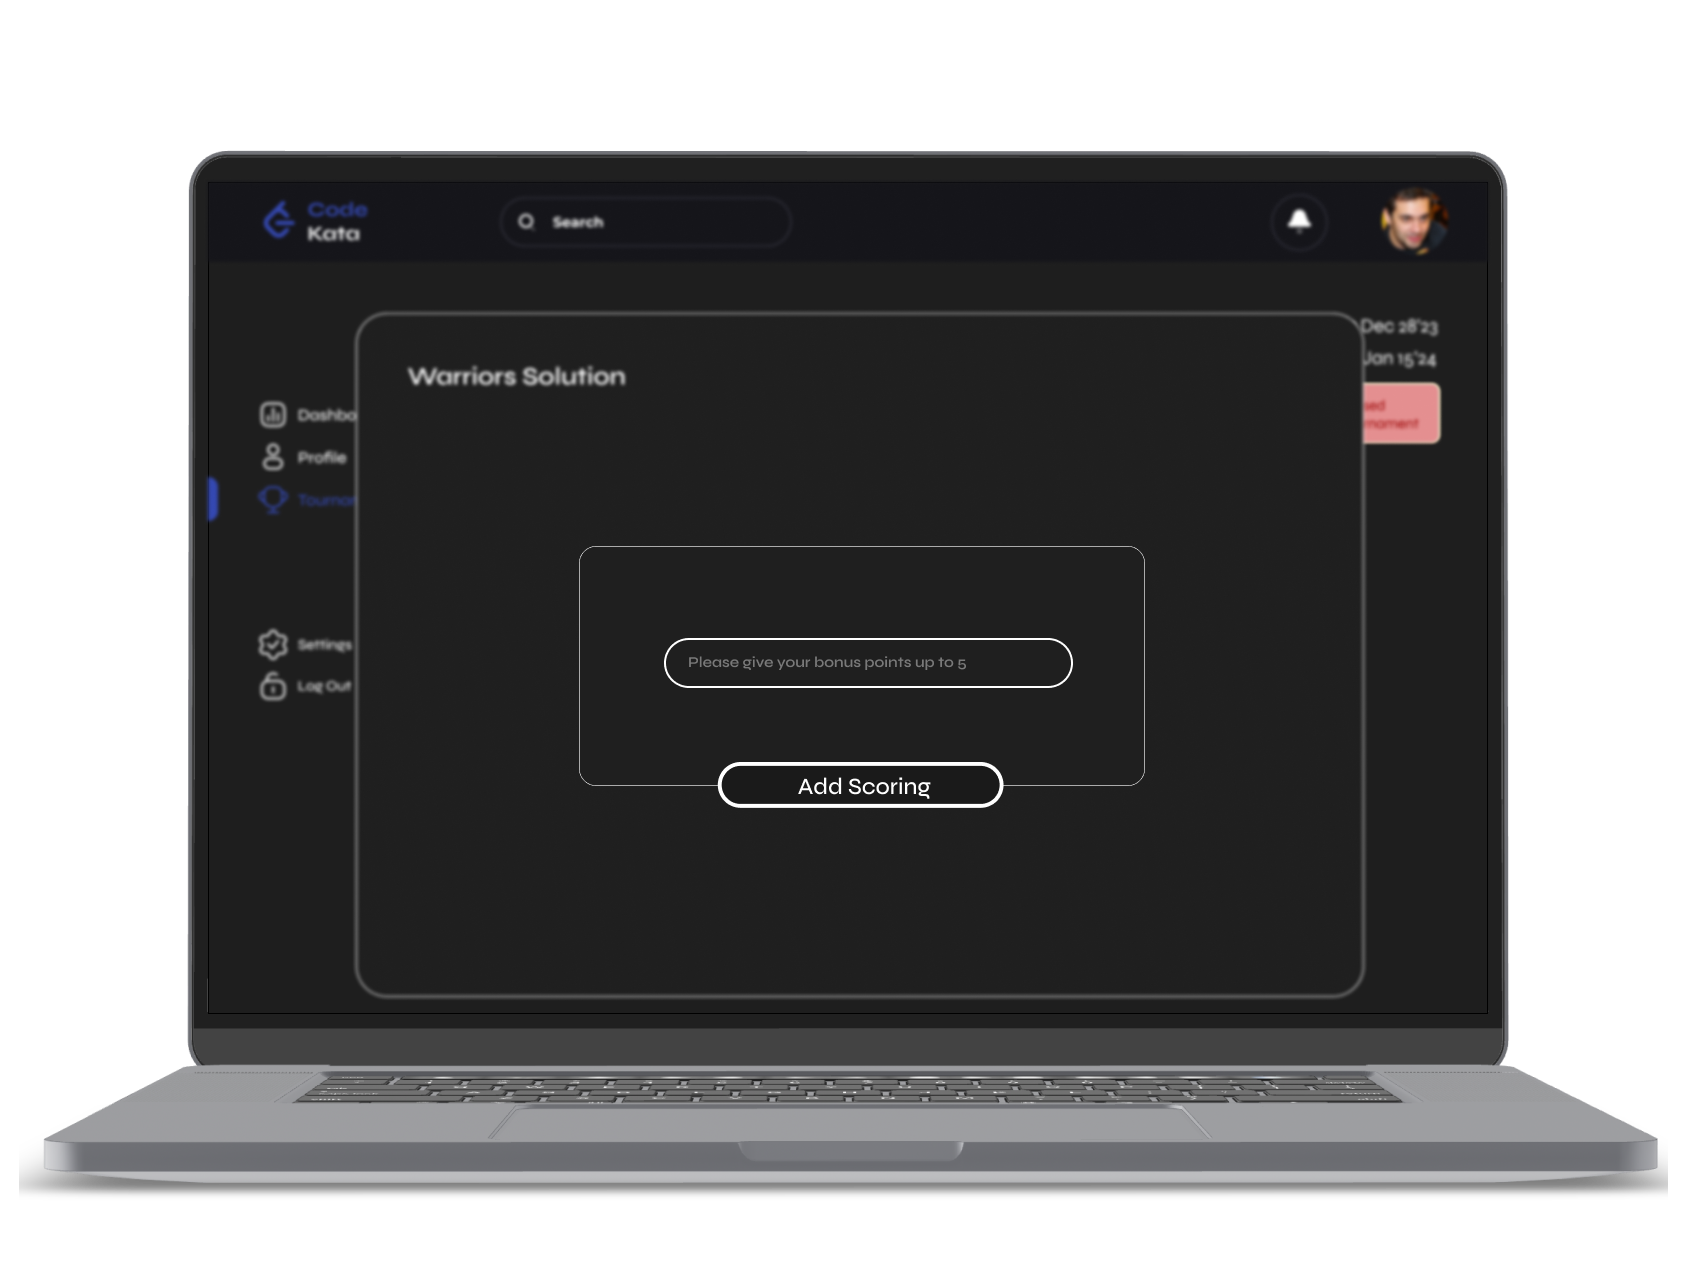
\includegraphics[scale=0.13]{Images/ui-ux/educator_team/educator_team_3.png}
% 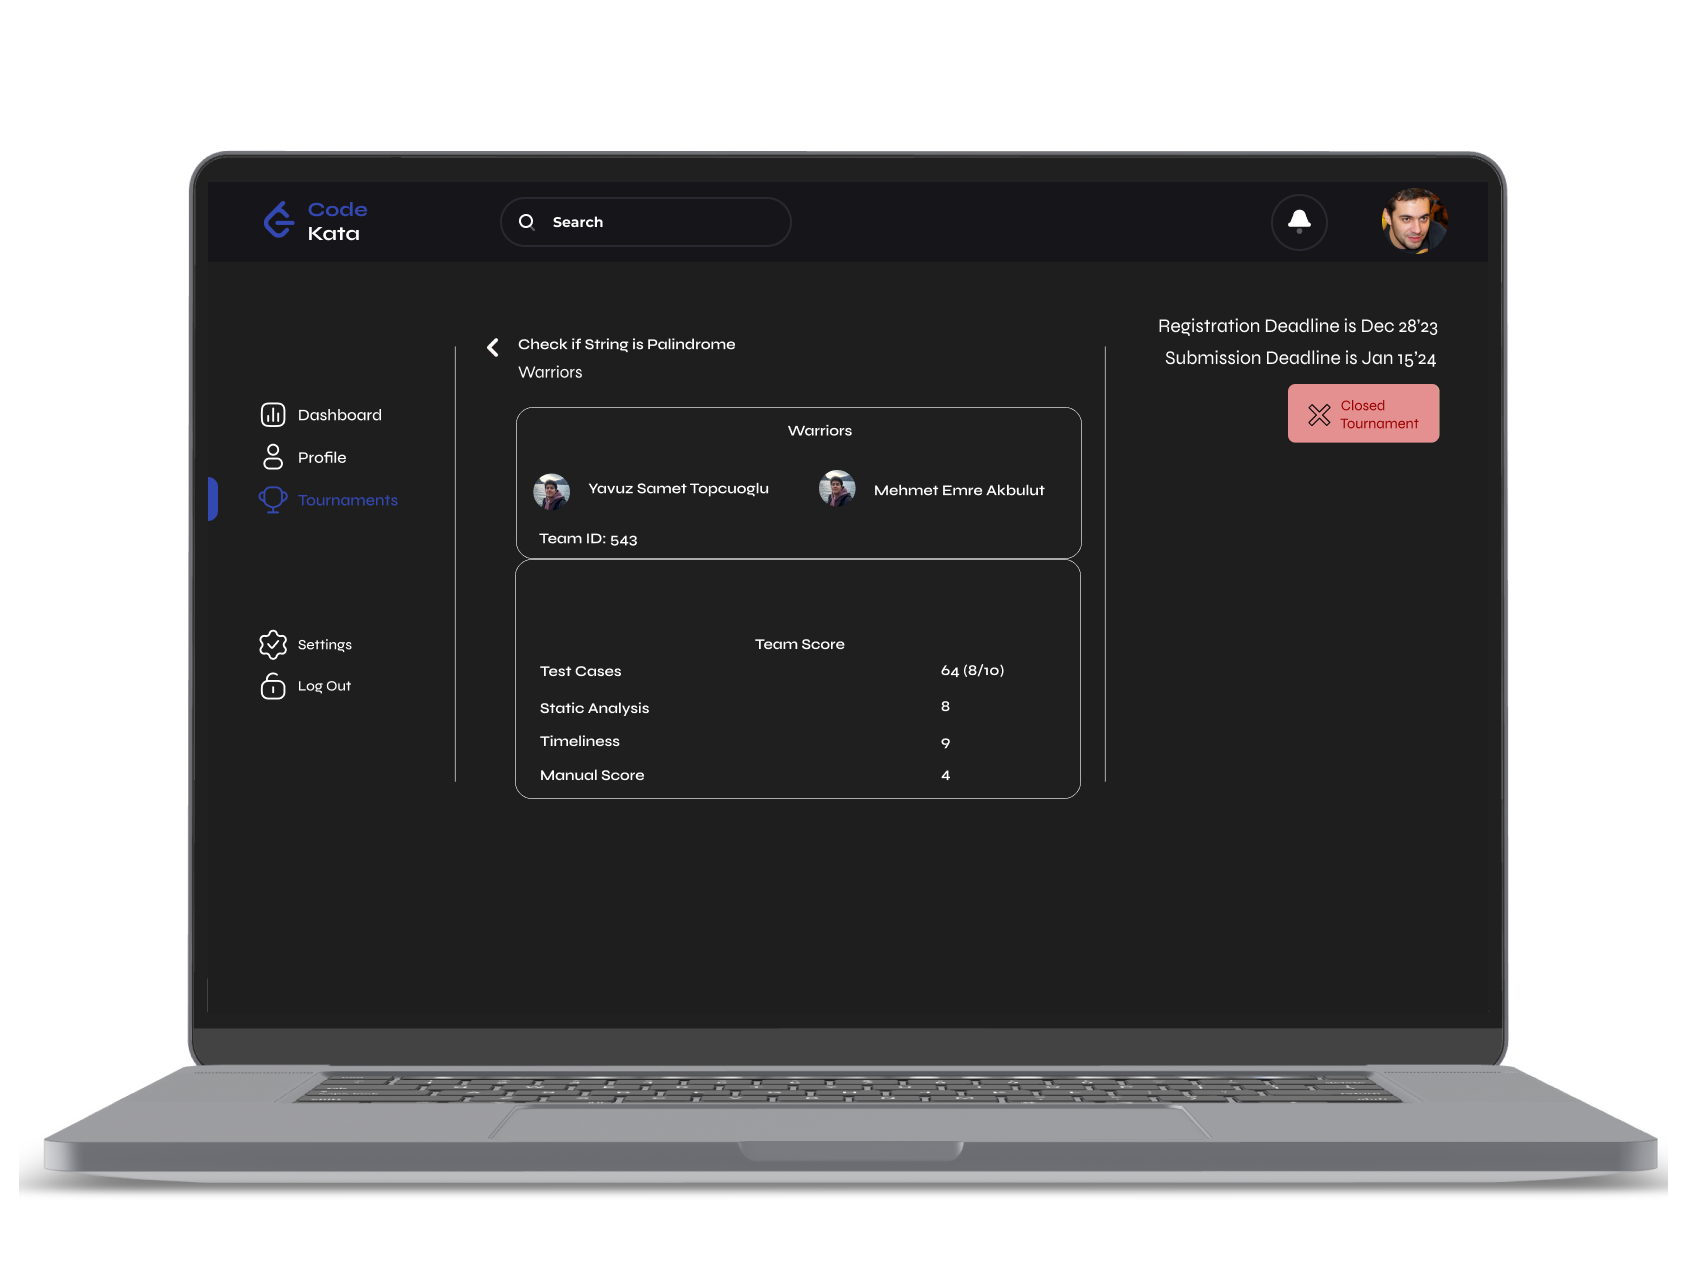
\includegraphics[scale=0.13]{Images/ui-ux/educator_team/educator_team_4.png}
%         (a) Educator, Team and Manual Scoring
% \end{center}
% \begin{center}
% 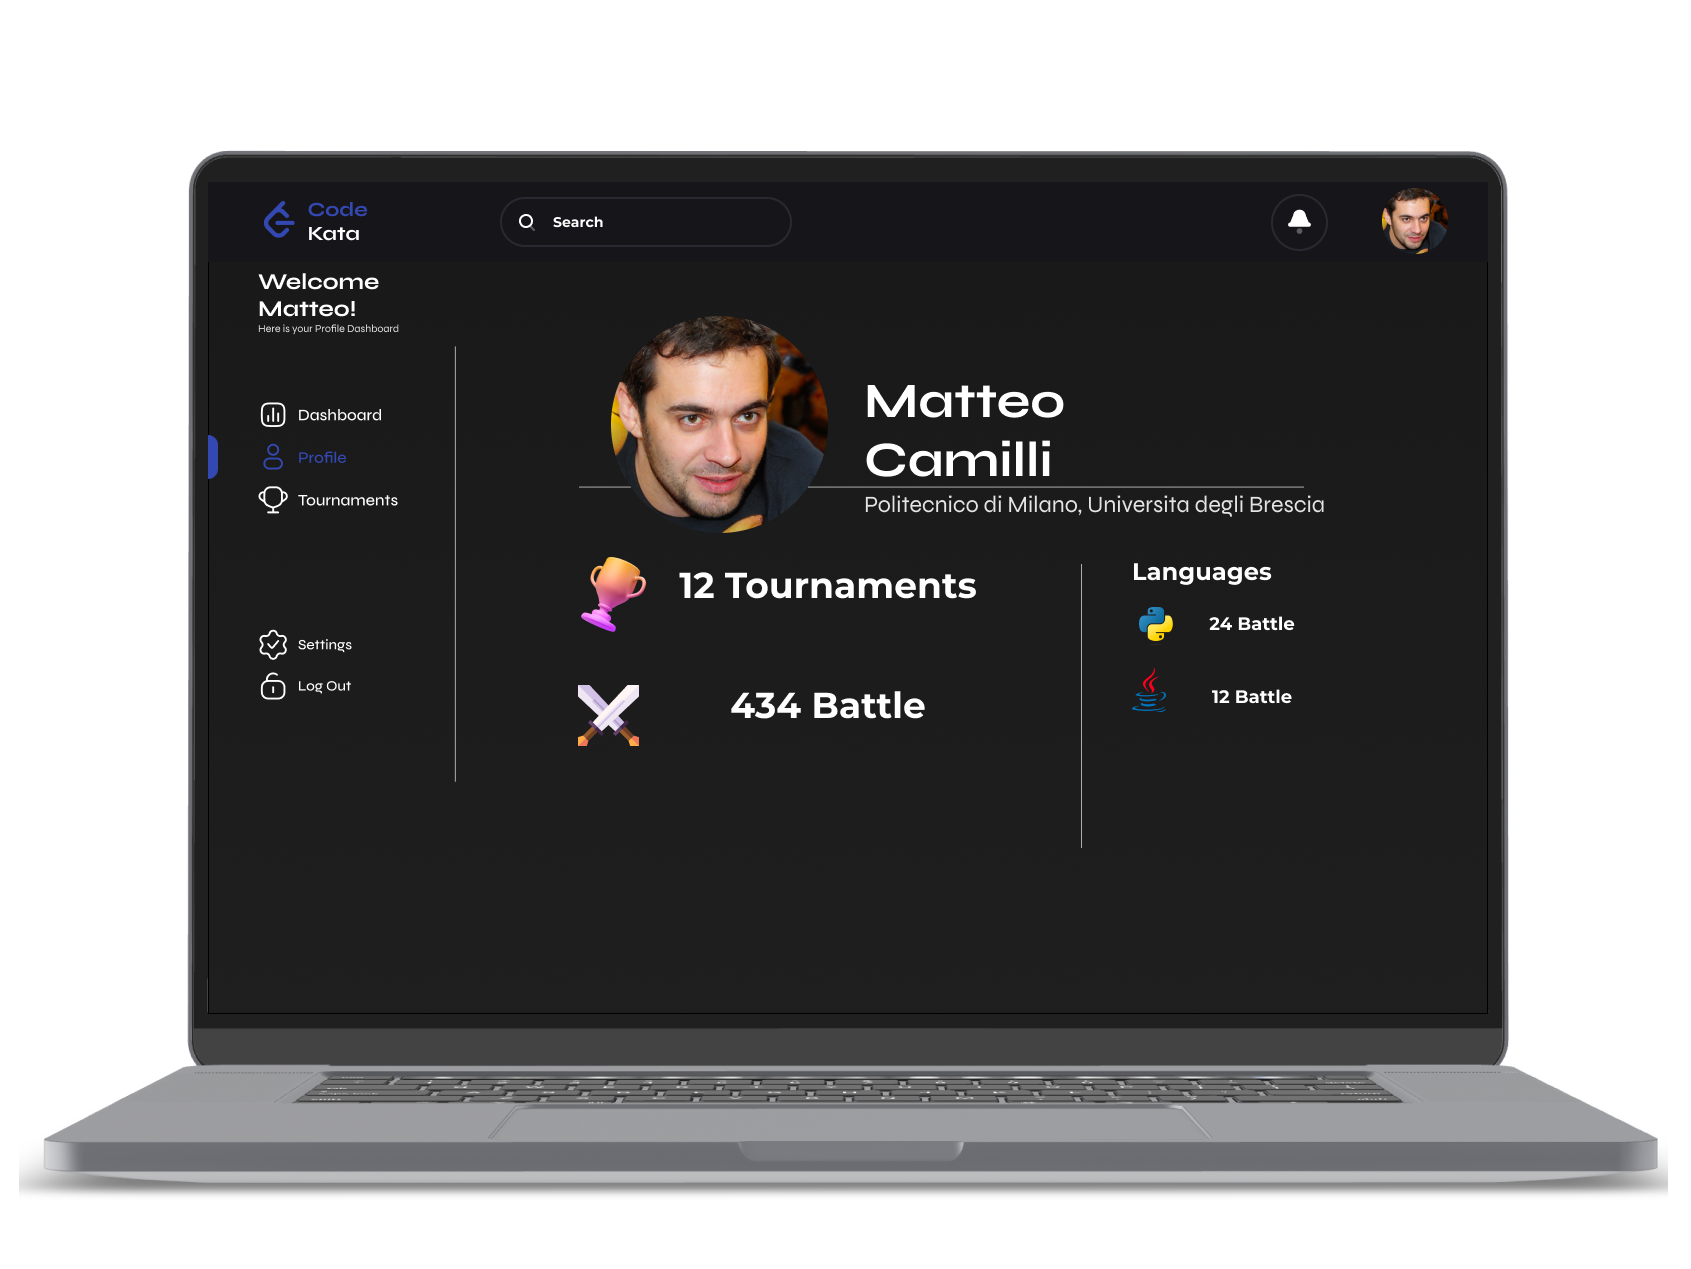
\includegraphics[scale=0.13]{Images/ui-ux/educator_profile_settings/educator_profile.png}
% 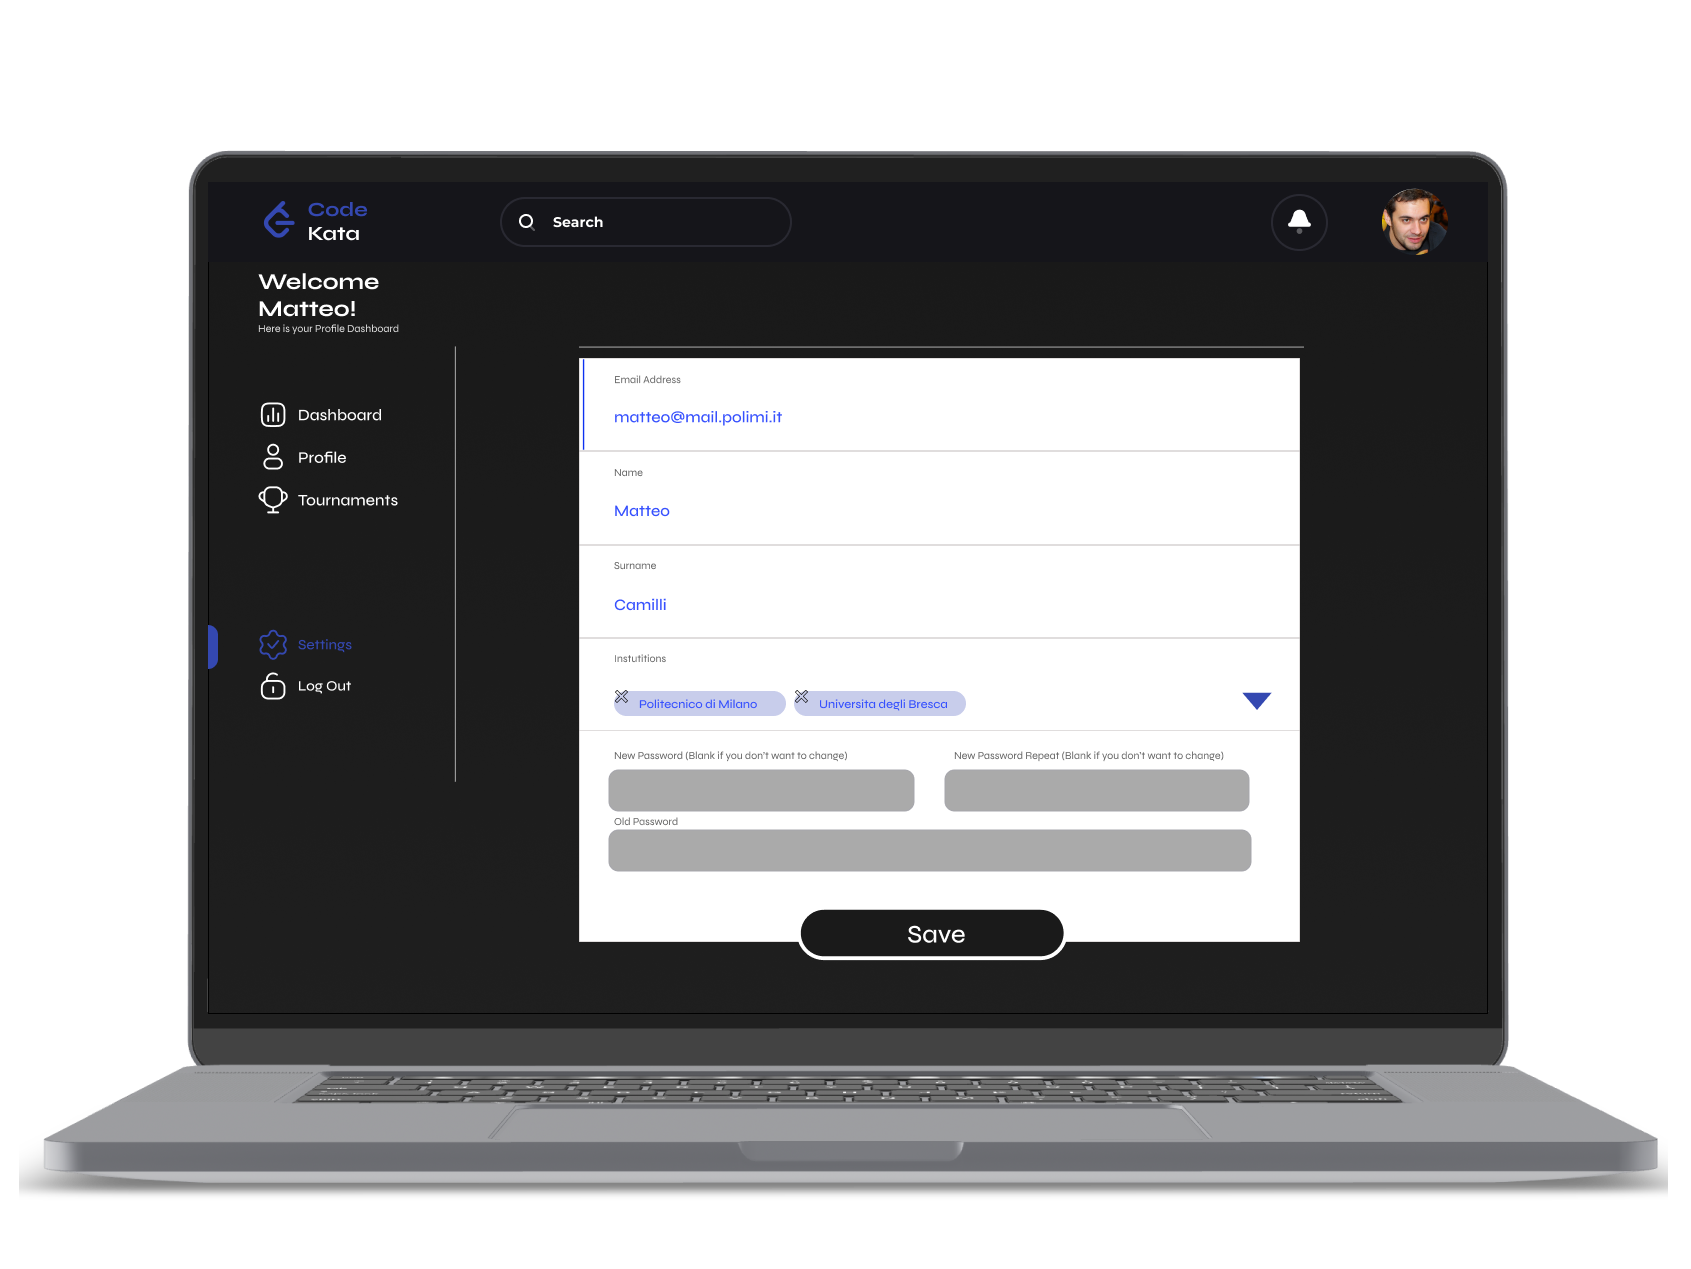
\includegraphics[scale=0.13]{Images/ui-ux/educator_profile_settings/educator_settings.png}
%         (a) Educator Profile and Settings
% \end{center}
\newpage
    
\subsubsection{Hardware Interfaces}
The CodeKataBattle platform operates entirely through web interfaces, eliminating the need for specialized hardware interfaces. Users can access the platform using standard web-enabled devices, such as computers, tablets, and smartphones. The platform is designed to function within a web browser, requiring no specific hardware beyond a device capable of running a modern browser and accessing the internet. This approach ensures broad accessibility without necessitating particular hardware configurations, making the platform versatile and user-friendly across various hardware setups. However, for optimal experience, at least 2GB of RAM and a minimum of 1GB of free space are recommended for browser caching and temporary files.

\subsubsection{Software Interfaces}
Our platform CKB interfaces with various software systems:

\begin{itemize}
    \item \textbf{Web Browsers:} Platform operates on web browsers. For universal access and easy use, it is compatible with major browsers like Chrome, Edge, Safari, Opera, and Firefox.

    \item \textbf{GitHub API:} Integrated for creating coding repositories and managing code \textit{submission} processes.

    \item \textbf{Sandboxing:} To create an isolated testing environment, our Sandbox Manager will utilise Docker.

    \item \textbf{Static Analysis Tool:} SonarQube API will be integrated for scoring the quality aspect of the code with static analysis. 

    \item \textbf{Database Technology:} Platform uses databases such as PostgreSQL.

    \item \textbf{Hosting:} Our platform uses Amazon Web Services EC2 for web server and database hosting.

    \item \textbf{Cloud File Storage:} The files will be stored using Amazon S3 services.

    \item \textbf{Email Service:} Amazon Simple Email Service SES will be used to send automated email notifications.
\end{itemize}

\subsubsection{Communication Interfaces}
Our platform utilises various communication systems:

\begin{itemize}
    \item \textbf{HTTPS:} For secure connection over the internet.

    \item \textbf{RESTful APIs:} We have RESTful APIs to communicate with the requests coming from GitHub Actions and the web application.

    \item \textbf{SMTP:} It is used to manage to send automated emails.
\end{itemize}





\subsection{Functional Requirements}
\subsubsection{Use Case Diagrams}
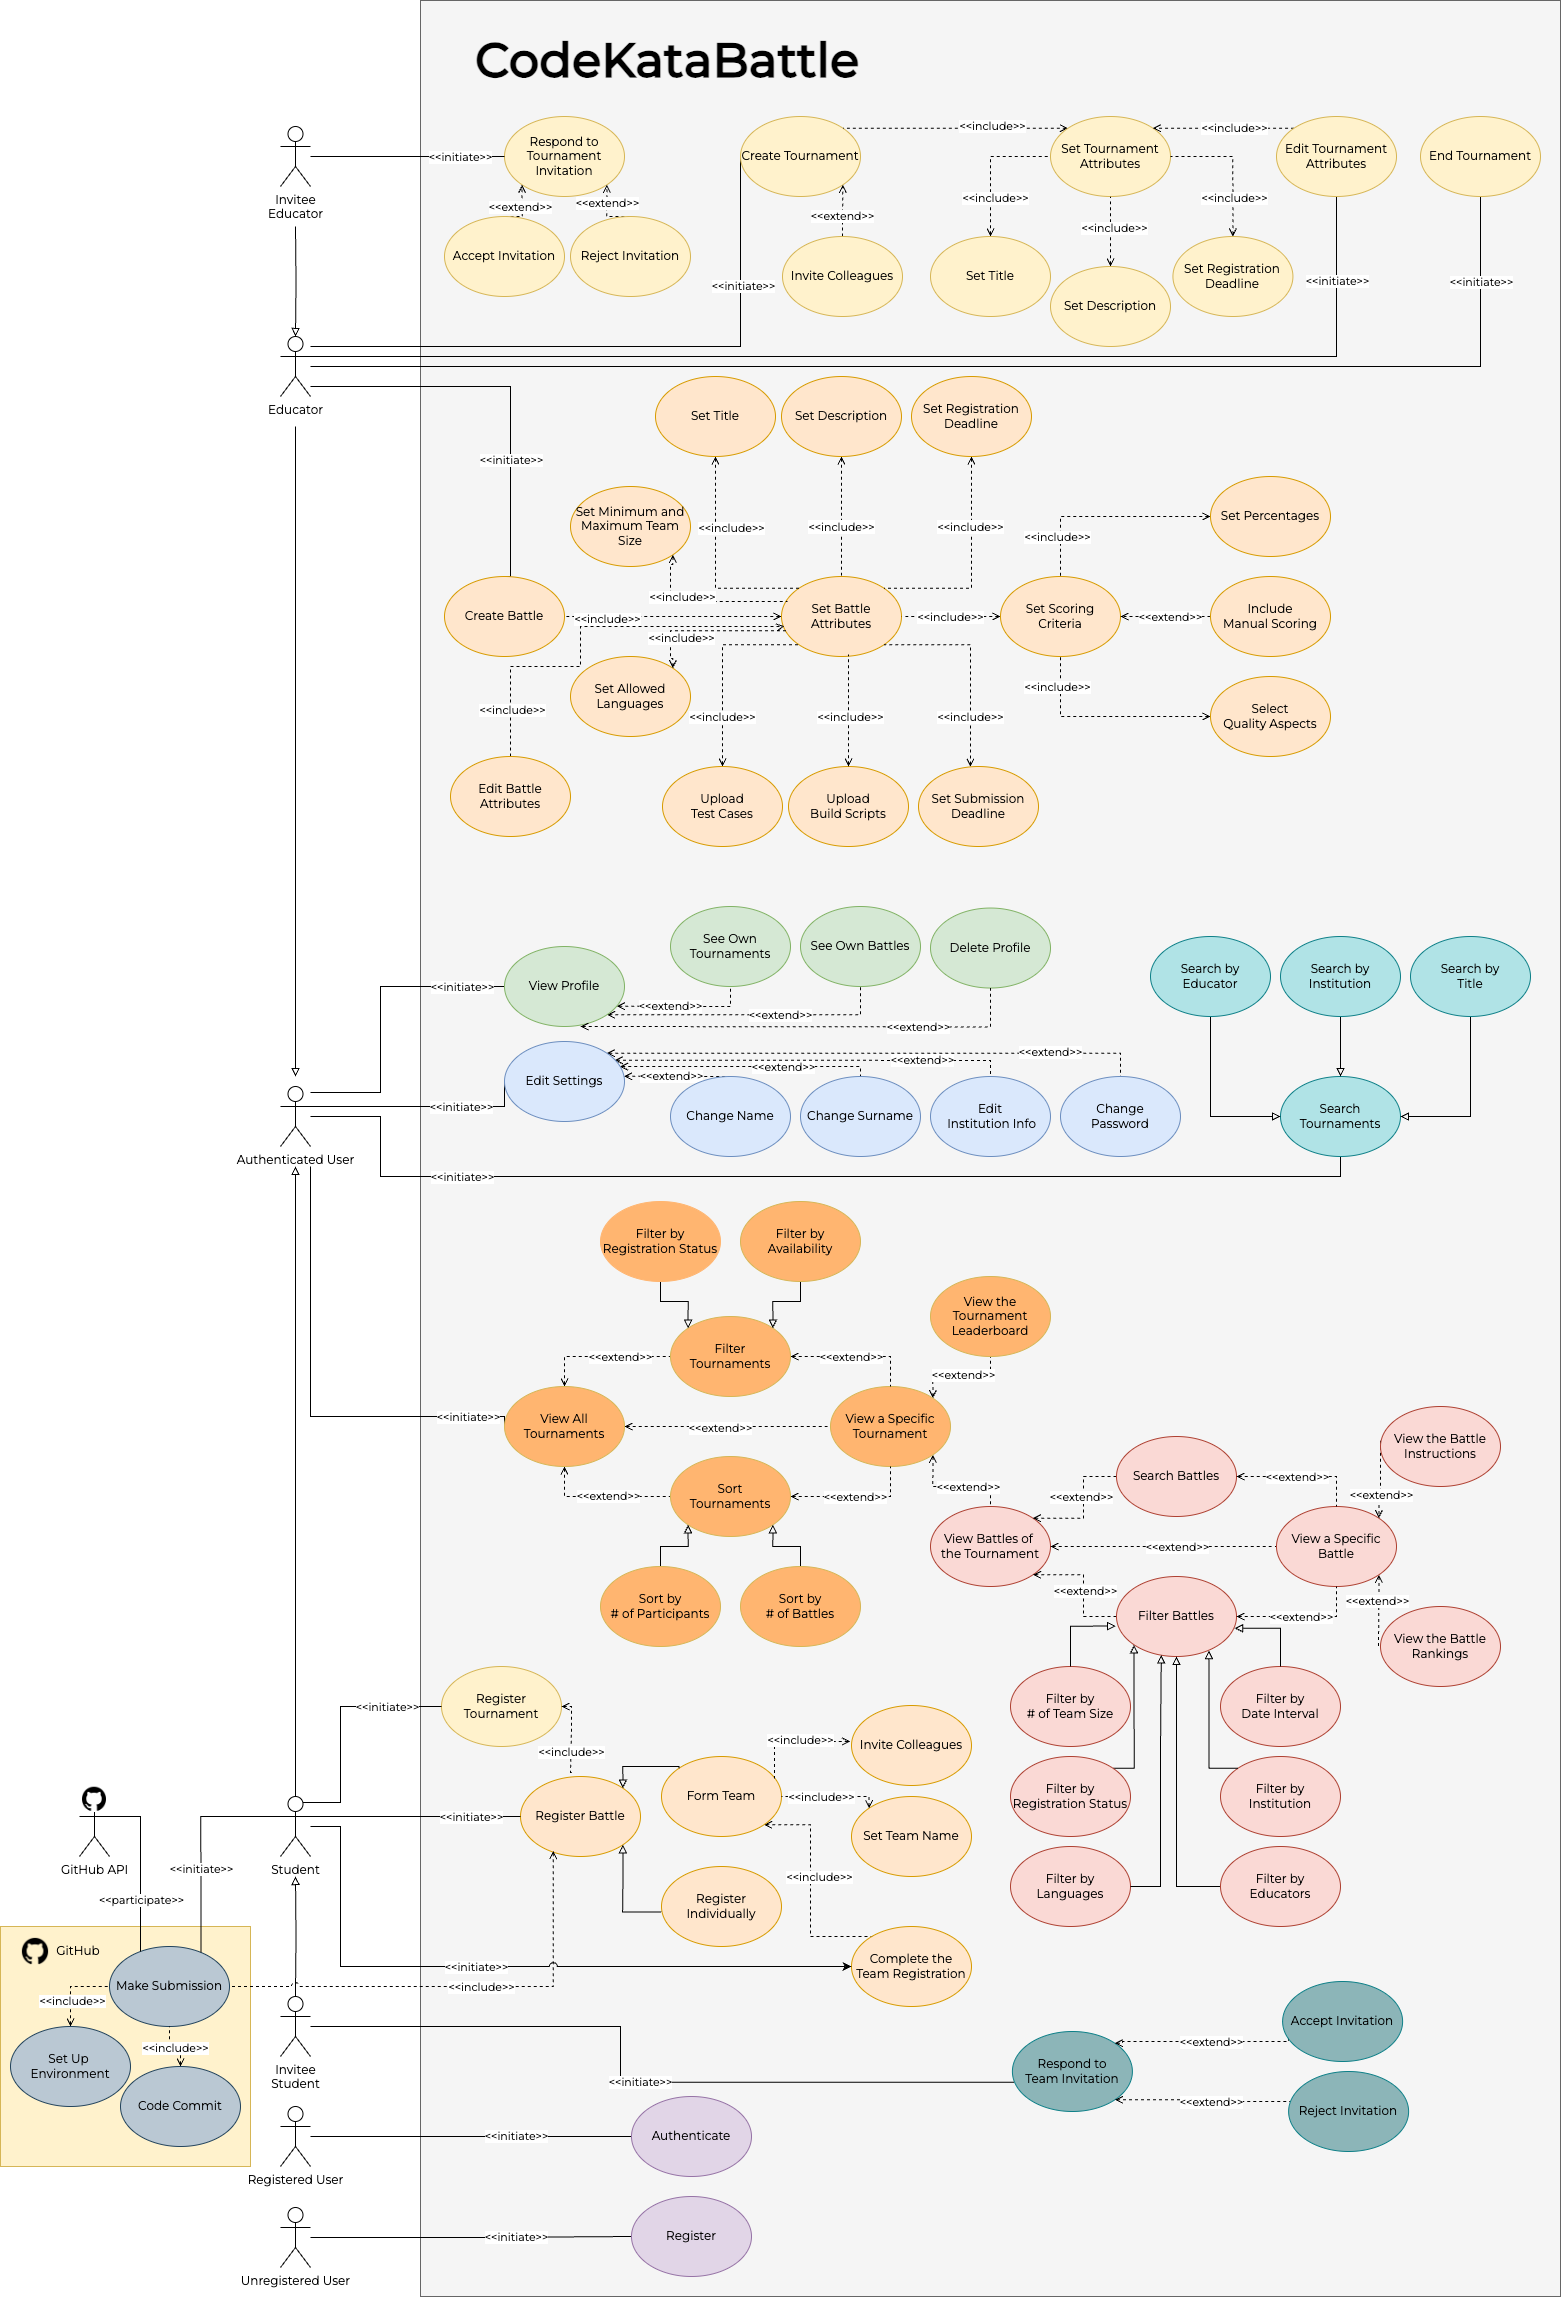
\includegraphics[scale=0.27]{Images/use-case-diagrams.drawio.png}
\newpage
\quad Unregistered User Actor has been used to illustrate the Registration Use Case. Similarly, the Registered User Actor has been used to show the Authentication Use Case. Other user actors are assumed to be registered and authenticated.

\quad Our system is composed of two main user types: Student and Educator. In the use case diagram, we showed common use cases with the Authenticated User actor. Authenticated User, simply every user registered to the platform, can view Tournaments, Battles, and their rankings with different filters and search options. Moreover, Registered User has the capability of viewing their profile and editing settings.

\quad Use case related Educator and Student Actors summarizes the goal of these users in the system.

\quad Invitee Student and Invitee Educator Actors are used to demonstrate use cases for tournament (for educators) and team (for students) invitations.

\quad GitHub System Boundary contains use cases about code submission with the participation of GitHub API Actor.


\subsubsection{Use Cases}

TEMPLATE:

\begin{center}
    \begin{tabular}{ | m{10em} | m{10cm}| } 
      \hline
      \textbf{Name} & exp  \\ 
      \hline
      \textbf{Actor(s)} & exp \\ 
      \hline
      \textbf{Entry Condition} & exp \\ 
      \hline
      \textbf{Event Flow} & 
          \begin{enumerate}[(1)]
              \item 
          \end{enumerate}
      \\ 
      \hline
      \textbf{Exit Condition} & exp  \\ 
      \hline
      \textbf{Exception(s)} & 
      \begin{itemize}
          \item 
      \end{itemize}
          \\ 
      \hline
      \textbf{Related Use Case(s)} & 
      \begin{itemize}
          \item 
      \end{itemize}
          \\ 
      \hline
      \textbf{Note(s)} & 
      \begin{itemize}
          \item 
      \end{itemize}
          \\ 
      \hline
    \end{tabular}
\end{center}

\begin{enumerate}
    \item Register
    \begin{center}
        \begin{tabular}{ | m{10em} | m{10cm}| } 
          \hline
          \textbf{Name} & Register  \\ 
          \hline
         \textbf{Actor(s)} & Unregistered User \\ 
          \hline
          \textbf{Entry Condition} & The user is unregistered to the platform. \\ 
          \hline
          \textbf{Event Flow} & 
          \begin{enumerate}[(1)]
              \item The actor enters the platform and clicks the Sign Up button.
              \item The actor fills out the registration form by providing email, password, name, surname, and institution information.
              \item The actor clicks the Sign Up button.
          \end{enumerate} \\
          \hline
          \textbf{Exit Condition} & The actor is registered and the Login page is displayed.  \\ 
          \hline
          \textbf{Exception(s)} & 
          \begin{itemize}
          \item 
      \end{itemize}
      \\ 
          \hline
          \textbf{Related Use Case(s)} & \begin{itemize}
          \item 
      \end{itemize}  \\ 
          \hline
          \textbf{Note(s)} & \begin{itemize}
          \item 
      \end{itemize}  \\ 
          \hline
        \end{tabular}
    \end{center}


    \item Login
    \begin{center}
    \begin{tabular}{ | m{10em} | m{10cm}| } 
      \hline
      \textbf{Name} & Login (i.e. Authenticate)  \\ 
      \hline
      \textbf{Actor(s)} & Registered User \\ 
      \hline
      \textbf{Entry Condition} & The user is already registered to the platform. \\ 
      \hline
      \textbf{Event Flow} & 
          \begin{enumerate}[(1)]
              \item The actor enters the platform web page.
              \item The actor fills out the form by providing an email address and a password.
              \item The actor clicks the Login button.
          \end{enumerate}
      \\ 
      \hline
      \textbf{Exit Condition} & The actor is logged in and the dashboard is displayed.  \\ 
      \hline
      \textbf{Exception(s)} & 
      \begin{itemize}
          \item The email and password do not match.
      \end{itemize}
      \\ 
      \hline
      \textbf{Related Use Case(s)} & 
      \begin{itemize}
          \item 
      \end{itemize}
      \\ 
      \hline
      \textbf{Note(s)} & 
      \begin{itemize}
          \item 
      \end{itemize}
      \\ 
      \hline
    \end{tabular}
\end{center}

\item View a Tournament
    \begin{center}
    \begin{tabular}{ | m{10em} | m{10cm}| } 
      \hline
      \textbf{Name} & View a Tournament  \\ 
      \hline
      \textbf{Actor(s)} & Authenticated User \\ 
      \hline
      \textbf{Entry Condition} & The actor is logged in. \\ 
      \hline
      \textbf{Event Flow} & 
          \begin{enumerate}[(1)]
              \item The actor clicks the Tournaments button from the sidebar.
              \item In the tournaments page, the actor \textit{views all tournaments} as cards.
              \item The actor \textit{filters tournaments} by registered filter.
              \item The actor \textit{sorts tournaments} by # of participants.
              \item The actor clicks the first tournament card to \textit{view a specific tournament}.
          \end{enumerate}
      \\ 
      \hline
      \textbf{Exit Condition} & The specific tournament that the actor wants to view is displayed.  \\ 
      \hline
      \textbf{Exception(s)} & 
      \begin{itemize}
          \item There are no existing tournaments.
          \item There are no tournaments with the filter set by the actor.
      \end{itemize}
          \\ 
      \hline
      \textbf{Related Use Case(s)} & 
      \begin{itemize}
          \item 
      \end{itemize}
          \\ 
      \hline
      \textbf{Note(s)} & 
      \begin{itemize}
          \item 
      \end{itemize}
          \\ 
      \hline
    \end{tabular}
\end{center}

\item View the Tournament Leaderboard
\begin{center}
    \begin{tabular}{ | m{10em} | m{10cm}| } 
      \hline
      \textbf{Name} & View the Tournament Leaderboard \\ 
      \hline
      \textbf{Actor(s)} & Authenticated User \\ 
      \hline
      \textbf{Entry Condition} & The actor is viewing a specific tournament. \\ 
      \hline
      \textbf{Event Flow} & 
          \begin{enumerate}[(1)]
              \item The actor clicks the Leaderboard button to \textit{view the tournament leaderboard}.
          \end{enumerate}
      \\ 
      \hline
      \textbf{Exit Condition} & The leaderboard of that tournament is displayed.  \\ 
      \hline
      \textbf{Exception(s)} & 
      \begin{itemize}
          \item 
      \end{itemize}
          \\ 
      \hline
      \textbf{Related Use Case(s)} & 
      \begin{itemize}
          \item 
      \end{itemize}
          \\ 
      \hline
      \textbf{Note(s)} & 
      \begin{itemize}
          \item 
      \end{itemize}
          \\ 
      \hline
    \end{tabular}
\end{center}


\item View a Battle
    \begin{center}
    \begin{tabular}{ | m{10em} | m{10cm}| } 
      \hline
      \textbf{Name} & View a Battle  \\ 
      \hline
      \textbf{Actor(s)} & Authenticated User \\ 
      \hline
      \textbf{Entry Condition} & The actor is viewing a specific tournament. \\ 
      \hline
      \textbf{Event Flow} & 
          \begin{enumerate}[(1)]
              \item The actor can \textit{view battles of the tournament} in that tournament's page.
              \item The actor \textit{filters battles} using the filter section on the right-hand side of the page.
              \item The actor chooses one of the results to \textit{view a specific battle}.
          \end{enumerate}
      \\ 
      \hline
      \textbf{Exit Condition} & The specific battle that the actor wants to view is displayed.  \\ 
      \hline
      \textbf{Exception(s)} & 
      \begin{itemize}
          \item There are no existing battles in that tournament.
          \item There are no battles with the filters set by the actor.
      \end{itemize}
          \\ 
      \hline
      \textbf{Related Use Case(s)} & 
      \begin{itemize}
          \item 
      \end{itemize}
          \\ 
      \hline
      \textbf{Note(s)} & 
      \begin{itemize}
          \item 
      \end{itemize}
          \\ 
      \hline
    \end{tabular}
\end{center}


\item View the Battle Instructions
\begin{center}
    \begin{tabular}{ | m{10em} | m{10cm}| } 
      \hline
      \textbf{Name} & View the Battle Instructions \\ 
      \hline
      \textbf{Actor(s)} & Authenticated User \\ 
      \hline
      \textbf{Entry Condition} & The actor is viewing a specific battle. \\ 
      \hline
      \textbf{Event Flow} & 
          \begin{enumerate}[(1)]
              \item The actor clicks the Instructions button to \textit{view the battle instructions}.
          \end{enumerate}
      \\ 
      \hline
      \textbf{Exit Condition} & The instructions of that battle are displayed.  \\ 
      \hline
      \textbf{Exception(s)} & 
      \begin{itemize}
          \item 
      \end{itemize}
          \\ 
      \hline
      \textbf{Related Use Case(s)} & 
      \begin{itemize}
          \item 
      \end{itemize}
          \\ 
      \hline
      \textbf{Note(s)} & 
      \begin{itemize}
          \item 
      \end{itemize}
          \\ 
      \hline
    \end{tabular}
\end{center}

\item View the Battle Rankings
\begin{center}
    \begin{tabular}{ | m{10em} | m{10cm}| } 
      \hline
      \textbf{Name} & View the Battle Rankings \\ 
      \hline
      \textbf{Actor(s)} & Authenticated User \\ 
      \hline
      \textbf{Entry Condition} & The actor is viewing a specific battle. \\ 
      \hline
      \textbf{Event Flow} & 
          \begin{enumerate}[(1)]
              \item The actor clicks the Scores button to \textit{view the battle rankings}.
          \end{enumerate}
      \\ 
      \hline
      \textbf{Exit Condition} & The rankings of that battle are displayed.  \\ 
      \hline
      \textbf{Exception(s)} & 
      \begin{itemize}
          \item 
      \end{itemize}
          \\ 
      \hline
      \textbf{Related Use Case(s)} & 
      \begin{itemize}
          \item 
      \end{itemize}
          \\ 
      \hline
      \textbf{Note(s)} & 
      \begin{itemize}
          \item 
      \end{itemize}
          \\ 
      \hline
    \end{tabular}
\end{center}


\item Search Tournaments
\begin{center}
    \begin{tabular}{ | m{10em} | m{10cm}| } 
      \hline
      \textbf{Name} & Search Tournament  \\ 
      \hline
      \textbf{Actor(s)} & Authenticated User \\ 
      \hline
      \textbf{Entry Condition} & The user is logged in. \\ 
      \hline
      \textbf{Event Flow} & 
          \begin{enumerate}[(1)]
              \item The actor clicks the button in the search area to select the search criteria.
              \item The actor sees three buttons: \textit{Search by Educators}, \textit{Search by Titles}, \textit{Search by Institutions} and chooses to search by title.
              \item The actor writes "Fall'23 Tournament" to the search bar and hits enter to search.
          \end{enumerate}
      \\ 
      \hline
      \textbf{Exit Condition} & The tournaments with the corresponding title are displayed.  \\ 
      \hline
      \textbf{Exception(s)} & 
      \begin{itemize}
          \item The tournament with the given title does not exist.
      \end{itemize}
          \\ 
      \hline
      \textbf{Related Use Case(s)} & 
      \begin{itemize}
          \item 
      \end{itemize}
          \\ 
      \hline
      \textbf{Note(s)} & 
      \begin{itemize}
          \item 
      \end{itemize}
          \\ 
      \hline
    \end{tabular}
\end{center}


\item Register to a Tournament
\begin{center}
    \begin{tabular}{ | m{10em} | m{10cm}| } 
      \hline
      \textbf{Name} & Register to a Tournament  \\ 
      \hline
      \textbf{Actor(s)} & Student \\ 
      \hline
      \textbf{Entry Condition} & The actor is logged in and the tournaments page is on display.\\ 
      \hline
      \textbf{Event Flow} & 
          \begin{enumerate}[(1)]
              \item The actor clicks a card of a tournament in which s/he is not registered.
              \item The actor clicks the Register button in the pop-up.
          \end{enumerate}
      \\ 
      \hline
      \textbf{Exit Condition} & The actor is registered to the tournament and the page of that tournament is displayed.  \\ 
      \hline
      \textbf{Exception(s)} & 
      \begin{itemize}
          \item There are not any tournaments with not registered status.
      \end{itemize}
          \\ 
      \hline
      \textbf{Related Use Case(s)} & 
      \begin{itemize}
          \item 
      \end{itemize}
          \\ 
      \hline
      \textbf{Note(s)} & 
      \begin{itemize}
          \item 
      \end{itemize}
          \\ 
      \hline
    \end{tabular}
\end{center}


\item Register to a Battle
\begin{center}
    \begin{tabular}{ | m{10em} | m{10cm}| } 
      \hline
      \textbf{Name} & Register to a Battle  \\ 
      \hline
      \textbf{Actor(s)} & Student \\ 
      \hline
      \textbf{Entry Condition} & The actor registered to the tournament in which the battle takes place and that tournament's page is on display. \\ 
      \hline
      \textbf{Event Flow} & 
          \begin{enumerate}[(1)]
              \item The actor clicks a register button next to the battle that s/he wants to participate in.
              \item The actor clicks the Register button in the pop-up.
              \item The actor chooses between to \textit{form a team} and to \textit{register individually}. 
              \item If there is going to be a team, the actor \textit{sets a team name} and \textit{invites colleagues}.
              \item The actor clicks the Complete button.
          \end{enumerate}
      \\ 
      \hline
      \textbf{Exit Condition} & 
      \begin{itemize}
          \item If registered individually, the actor is registered to the battle.
          \item If a team is formed, the invitation requests are sent to the colleagues.
      \end{itemize}
        \\ 
      \hline
      \textbf{Exception(s)} & 
      \begin{itemize}
          \item The actor is already registered for all battles in that tournament.
      \end{itemize}
          \\ 
      \hline
      \textbf{Related Use Case(s)} & 
      \begin{itemize}
          \item 
      \end{itemize}
          \\ 
      \hline
      \textbf{Note(s)} & 
      \begin{itemize}
          \item 
      \end{itemize}
          \\ 
      \hline
    \end{tabular}
\end{center}



\item Complete the Team Registration for the Battle
\begin{center}
    \begin{tabular}{ | m{10em} | m{10cm}| } 
      \hline
      \textbf{Name} & Complete the Team Registration for the Battle  \\ 
      \hline
      \textbf{Actor(s)} & Student \\ 
      \hline
      \textbf{Entry Condition} & The specific battle that the actor wants to complete the registration is on display. \\ 
      \hline
      \textbf{Event Flow} & 
          \begin{enumerate}[(1)]
              \item The actor can see which colleague accepted the invitation and which colleague rejected it.
              \item The actor can finalize the team formation if there are enough colleagues on the team by using the Finalize button, or discard the team and battle registration entirely by using the Decline button.
          \end{enumerate}
      \\ 
      \hline
      \textbf{Exit Condition} & 
      \begin{itemize}
          \item If finalized, the team is registered to the battle.
          \item If declined, the team is not registered to the battle and the dashboard is displayed.
      \end{itemize}\\ 
      \hline
      \textbf{Exception(s)} & 
      \begin{itemize}
          \item 
      \end{itemize}
          \\ 
      \hline
      \textbf{Related Use Case(s)} & 
      \begin{itemize}
          \item 
      \end{itemize}
          \\ 
      \hline
      \textbf{Note(s)} & 
      \begin{itemize}
          \item 
      \end{itemize}
          \\ 
      \hline
    \end{tabular}
\end{center}


\item 


    

\end{enumerate}



